\documentclass[screen=true, natbib=false, 10pt, sigplan]{acmart}
\usepackage[utf8]{inputenc}
\usepackage[T1]{fontenc}

\newcommand{\packageGraphicx}{\usepackage{graphicx}}
\newcommand{\packageHyperref}{\usepackage{hyperref}}
\newcommand{\renewrmdefault}{\renewcommand{\rmdefault}{ptm}}
\newcommand{\packageRelsize}{\usepackage{relsize}}
% amsmath is required for the combination of {mathabx,
% wasysym, newtxmath} to work. Otherwise, newtxmath
% would load amsmath *after* mathabx and wasysym,
% causing command redefinition issues.
\newcommand{\packageAmsmath}{\usepackage{amsmath}}
\newcommand{\packageMathabx}{\usepackage{mathabx}}
% Avoid conflicts between "mathabx" and "wasysym",
% and between "wasysym" integrals and "amsmath" integrals (iint).
\newcommand{\packageWasysym}{
  \let\leftmoon\relax \let\rightmoon\relax \let\fullmoon\relax \let\newmoon\relax \let\diameter\relax
  \usepackage[nointegrals]{wasysym}}
% Both newtxmath and mathabx define the \widering command.
% The only reason we choose the newtxmath version is that
% acmart.cls is also using the one from newtxmath.
\newcommand{\packageTxfonts}{
  \let\widering\relax
  \usepackage{newtxmath}}
\newcommand{\packageTextcomp}{\usepackage{textcomp}}
\newcommand{\packageFramed}{\usepackage{framed}}
\newcommand{\packageHyphenat}{\usepackage[htt]{hyphenat}}
\newcommand{\packageColor}{\usepackage[usenames,dvipsnames]{color}}
\newcommand{\doHypersetup}{\hypersetup{bookmarks=true,bookmarksopen=true,bookmarksnumbered=true}}
\newcommand{\packageTocstyle}{\IfFileExists{tocstyle.sty}{\usepackage{tocstyle}\usetocstyle{standard}}{}}
\newcommand{\packageCJK}{\IfFileExists{CJK.sty}{\usepackage{CJK}}{}}
%%%%%%%%%%%%%%%%%%%%%%%%%%%%%%%%%%%%%%%%%%%%%%%%%%%%%%%%%%%%%%%%%%%%%%%%%%%%%%%%
% BEGIN acmart-load.tex
% Avoid package option conflict
\renewcommand\packageColor\relax
\renewcommand\packageTocstyle\relax
\renewcommand\packageMathabx{\ifx\bigtimes\undefined \usepackage{mathabx} \else \relax \fi}
% Both 'mathabx' and 'newtxmath' (required by the 'acmart' class) define a '\bigtimes' command. 
\renewcommand\packageTxfonts\relax
\let\Footnote\undefined
\let\captionwidth\undefined
\renewcommand{\renewrmdefault}{}
% END acmart-load.tex
%%%%%%%%%%%%%%%%%%%%%%%%%%%%%%%%%%%%%%%%%%%%%%%%%%%%%%%%%%%%%%%%%%%%%%%%%%%%%%%%
% This is the default style configuration for Scribble-generated Latex

\packageGraphicx
\packageHyperref
\renewrmdefault
\packageRelsize
\packageAmsmath
\packageMathabx
\packageWasysym
\packageTxfonts
\packageTextcomp
\packageFramed
\packageHyphenat
\packageColor
\doHypersetup
\packageTocstyle
\packageCJK


%%%%%%%%%%%%%%%%%%%%%%%%%%%%%%%%%%%%%%%%%%%%%%%%%%%%%%%%%%%%%%%%%%%%%%%%%%%%%%%%
% Configuration that is especially meant to be overridden:

% Inserted before every ``chapter'', useful for starting each one on a new page:
\newcommand{\sectionNewpage}{}
% Inserted before every book ``part''
\newcommand{\partNewpage}{\sectionNewpage}

% Hooks for actions within the `document' environment:
\newcommand{\preDoc}{}
\newcommand{\postDoc}{}

% Generated by `secref'; first arg is section number, second is section title:
\newcommand{\BookRef}[2]{\emph{#2}}
\newcommand{\ChapRef}[2]{\SecRef{#1}{#2}}
\newcommand{\SecRef}[2]{section~#1}
\newcommand{\PartRef}[2]{part~#1}
% Generated by `Secref':
\newcommand{\BookRefUC}[2]{\BookRef{#1}{#2}}
\newcommand{\ChapRefUC}[2]{\SecRefUC{#1}{#2}}
\newcommand{\SecRefUC}[2]{Section~#1}
\newcommand{\PartRefUC}[2]{Part~#1}

% Variants of the above with a label for an internal reference:
\newcommand{\BookRefLocal}[3]{\hyperref[#1]{\BookRef{#2}{#3}}}
\newcommand{\ChapRefLocal}[3]{\hyperref[#1]{\ChapRef{#2}{#3}}}
\newcommand{\SecRefLocal}[3]{\hyperref[#1]{\SecRef{#2}{#3}}}
\newcommand{\PartRefLocal}[3]{\hyperref[#1]{\PartRef{#2}{#3}}}
\newcommand{\BookRefLocalUC}[3]{\hyperref[#1]{\BookRefUC{#2}{#3}}}
\newcommand{\ChapRefLocalUC}[3]{\hyperref[#1]{\ChapRefUC{#2}{#3}}}
\newcommand{\SecRefLocalUC}[3]{\hyperref[#1]{\SecRefUC{#2}{#3}}}
\newcommand{\PartRefLocalUC}[3]{\hyperref[#1]{\PartRefUC{#2}{#3}}}

% Variants of the above with a section number is empty (i.e., UnNumbered):
\newcommand{\BookRefUN}[1]{\BookRef{}{#1}}
\newcommand{\ChapRefUN}[1]{\SecRefUN{#1}}
\newcommand{\SecRefUN}[1]{``#1''}
\newcommand{\PartRefUN}[1]{\SecRefUN{#1}}
\newcommand{\BookRefUCUN}[1]{\BookRefUN{#1}}
\newcommand{\ChapRefUCUN}[1]{\ChapRefUN{#1}}
\newcommand{\SecRefUCUN}[1]{\SecRefUN{#1}}
\newcommand{\PartRefUCUN}[1]{\PartRefUN{#1}}

\newcommand{\BookRefLocalUN}[2]{\hyperref[#1]{\BookRefUN{#2}}}
\newcommand{\ChapRefLocalUN}[2]{\SecRefLocalUN{#1}{#2}}
\newcommand{\SecRefLocalUN}[2]{\hyperref[#1]{\SecRefUN{#2}}}
\newcommand{\PartRefLocalUN}[2]{\SecRefLocalUN{#1}{#2}}
\newcommand{\BookRefLocalUCUN}[2]{\BookRefLocalUN{#1}{#2}}
\newcommand{\ChapRefLocalUCUN}[2]{\ChapRefLocalUN{#1}{#2}}
\newcommand{\SecRefLocalUCUN}[2]{\SecRefLocalUN{#1}{#2}}
\newcommand{\PartRefLocalUCUN}[2]{\PartRefLocalUN{#1}{#2}}

\newcommand{\SectionNumberLink}[2]{\hyperref[#1]{#2}}

% Enabled with a 'enable-index-merge part style property. This default
% implementation isn't good enough, because the argument is a
% comma-separated sequence of labels:
\newcommand{\Smanypageref}[1]{\pageref{#1}}

%%%%%%%%%%%%%%%%%%%%%%%%%%%%%%%%%%%%%%%%%%%%%%%%%%%%%%%%%%%%%%%%%%%%%%%%%%%%%%%%
% Fonts

% Font commands used by generated text:
\newcommand{\Scribtexttt}[1]{{\texttt{#1}}}
\newcommand{\textsub}[1]{$_{\hbox{\textsmaller{#1}}}$}
\newcommand{\textsuper}[1]{$^{\hbox{\textsmaller{#1}}}$}
\newcommand{\intextcolor}[2]{\textcolor{#1}{#2}}
\newcommand{\intextrgbcolor}[2]{\textcolor[rgb]{#1}{#2}}
\newcommand{\incolorbox}[2]{{\fboxrule=0pt\fboxsep=0pt\protect\colorbox{#1}{#2}}}
\newcommand{\inrgbcolorbox}[2]{{\fboxrule=0pt\fboxsep=0pt\protect\colorbox[rgb]{#1}{#2}}}
\newcommand{\plainlink}[1]{#1}
\newcommand{\techoutside}[1]{#1}
\newcommand{\techinside}[1]{#1}
\newcommand{\badlink}[1]{#1}
\newcommand{\indexlink}[1]{#1}
\newcommand{\noborder}[1]{#1}
\newcommand{\Smaller}[1]{\textsmaller{#1}}
\newcommand{\Larger}[1]{\textlarger{#1}}
\newcommand{\planetName}[1]{PLane\hspace{-0.1ex}T}
\newcommand{\slant}[1]{{\textsl{#1}}}

% Used for <, >, and | in tt mode. For some fonts and installations,
% there seems to be an encoding issue, so pick T1 explicitly:
\newcommand{\Stttextmore}{{\fontencoding{T1}\selectfont>}}
\newcommand{\Stttextless}{{\fontencoding{T1}\selectfont<}}
\newcommand{\Stttextbar}{{\fontencoding{T1}\selectfont|}}

%%%%%%%%%%%%%%%%%%%%%%%%%%%%%%%%%%%%%%%%%%%%%%%%%%%%%%%%%%%%%%%%%%%%%%%%%%%%%%%%
% Tables

% The `stabular' environment seems to be the lesser of evils among 
%  page-breaking table environments (and we've made a copy as ``pltstabular'
%  to make sure that it doesn't change).

\makeatletter
%%%%%%%%%%%%%%%%%%%%%%%%%%%%%%%%%%%%%%%%%%%%%%%%%%%%%%%%%%%%%%%%%%%%%%
\message{pltstabular is a modification of stabular}
%% A renamed version of:
%% stabular.sty
%% Copyright 1998 Sigitas Tolu\v sis
%% VTeX Ltd., Akademijos 4, Vilnius, Lithuania
%% e-mail sigitas@vtex.lt
%% http://www.vtex.lt/tex/download/macros/
%%
% This program can redistributed and/or modified under the terms
% of the LaTeX Project Public License Distributed from CTAN
% archives in directory macros/latex/base/lppl.txt; either
% version 1 of the License, or (at your option) any later version.
%
% PURPOSE:   Improve tabular environment.
%
% SHORT DESCRIPTION:
%
% Changed internal commands: \@mkpream, \@addamp, \@xhline
%
% Provides new commands in tabular (used after command \\):
% \emptyrow[#1] 
% -------------
%    Adds empty row, #1 - height of the row 
%
% \tabrow{#1}[#2] 
% ---------------
%    Adds row of natural height: #1\\[#2]
%
% Provides new environments: pltstabular and pltstabular* 
%                            --------     ---------
%            One more multi-page version of tabular
%
%
\def\empty@finalstrut#1{%
  \unskip\ifhmode\nobreak\fi\vrule\@width\z@\@height\z@\@depth\z@}
\def\no@strut{\global\setbox\@arstrutbox\hbox{%
    \vrule \@height\z@
           \@depth\z@
           \@width\z@}%
    \gdef\@endpbox{\empty@finalstrut\@arstrutbox\par\egroup\hfil}%
}%
\def\yes@strut{\global\setbox\@arstrutbox\hbox{%
    \vrule \@height\arraystretch \ht\strutbox
           \@depth\arraystretch \dp\strutbox
           \@width\z@}%
    \gdef\@endpbox{\@finalstrut\@arstrutbox\par\egroup\hfil}%
}%
\def\@mkpream#1{\@firstamptrue\@lastchclass6
  \let\@preamble\@empty\def\empty@preamble{\add@ins}%
  \let\protect\@unexpandable@protect
  \let\@sharp\relax\let\add@ins\relax
  \let\@startpbox\relax\let\@endpbox\relax
  \@expast{#1}%
  \expandafter\@tfor \expandafter
    \@nextchar \expandafter:\expandafter=\reserved@a\do
       {\@testpach\@nextchar
    \ifcase \@chclass \@classz \or \@classi \or \@classii \or \@classiii
      \or \@classiv \or\@classv \fi\@lastchclass\@chclass}%
  \ifcase \@lastchclass \@acol
      \or \or \@preamerr \@ne\or \@preamerr \tw@\or \or \@acol \fi}
\def\@addamp{%
  \if@firstamp
    \@firstampfalse
    \edef\empty@preamble{\add@ins}%
  \else
    \edef\@preamble{\@preamble &}%
    \edef\empty@preamble{\expandafter\noexpand\empty@preamble &\add@ins}%
  \fi}
\newif\iftw@hlines \tw@hlinesfalse
\def\@xhline{\ifx\reserved@a\hline
               \tw@hlinestrue
             \else\ifx\reserved@a\Hline
               \tw@hlinestrue
             \else
               \tw@hlinesfalse
             \fi\fi
      \iftw@hlines
        \aftergroup\do@after
      \fi
      \ifnum0=`{\fi}%
}
\def\do@after{\emptyrow[\the\doublerulesep]}
\def\emptyrow{\noalign\bgroup\@ifnextchar[\@emptyrow{\@emptyrow[\z@]}}
\def\@emptyrow[#1]{\no@strut\gdef\add@ins{\vrule \@height\z@ \@depth#1 \@width\z@}\egroup%
\empty@preamble\\
\noalign{\yes@strut\gdef\add@ins{\vrule \@height\z@ \@depth\z@ \@width\z@}}%
}
\def\tabrow#1{\noalign\bgroup\@ifnextchar[{\@tabrow{#1}}{\@tabrow{#1}[]}}
\def\@tabrow#1[#2]{\no@strut\egroup#1\ifx.#2.\\\else\\[#2]\fi\noalign{\yes@strut}}
%
\def\endpltstabular{\crcr\egroup\egroup \egroup}
\expandafter \let \csname endpltstabular*\endcsname = \endpltstabular
\def\pltstabular{\let\@halignto\@empty\@pltstabular}
\@namedef{pltstabular*}#1{\def\@halignto{to#1}\@pltstabular}
\def\@pltstabular{\leavevmode \bgroup \let\@acol\@tabacol
   \let\@classz\@tabclassz
   \let\@classiv\@tabclassiv \let\\\@tabularcr\@stabarray}
\def\@stabarray{\m@th\@ifnextchar[\@sarray{\@sarray[c]}}
\def\@sarray[#1]#2{%
  \bgroup
  \setbox\@arstrutbox\hbox{%
    \vrule \@height\arraystretch\ht\strutbox
           \@depth\arraystretch \dp\strutbox
           \@width\z@}%
  \@mkpream{#2}%
  \edef\@preamble{%
    \ialign \noexpand\@halignto
      \bgroup \@arstrut \@preamble \tabskip\z@skip \cr}%
  \let\@startpbox\@@startpbox \let\@endpbox\@@endpbox
  \let\tabularnewline\\%
%    \let\par\@empty
    \let\@sharp##%
    \set@typeset@protect
    \lineskip\z@skip\baselineskip\z@skip
    \@preamble}

%%%%%%%%%%%%%%%%%%%%%%%%%%%%%%%%%%%%%%%%%%%%%%%%%%%%%%%%%%%%%%%%%%%%%%
\makeatother

\newenvironment{bigtabular}{\begin{pltstabular}}{\end{pltstabular}}
% For the 'boxed table style:
\newcommand{\SBoxedLeft}{\textcolor[rgb]{0.6,0.6,1.0}{\vrule width 3pt\hspace{3pt}}}
% Formerly used to keep the horizontal line for a definition on the same page:
\newcommand{\SEndFirstHead}[0]{ \nopagebreak \\ }
% Corrects weirdness when a table is the first thing in
%  an itemization:
\newcommand{\bigtableinlinecorrect}[0]{~

\vspace{-\baselineskip}\vspace{\parskip}}
% Used to indent the table correctly in an itemization, since that's
%  one of the things stabular gets wrong:
\newlength{\stabLeft}
\newcommand{\bigtableleftpad}{\hspace{\stabLeft}}
\newcommand{\atItemizeStart}[0]{\addtolength{\stabLeft}{\labelsep}
                                \addtolength{\stabLeft}{\labelwidth}}


% For a single-column table in simple environments, it's better to
%  use the `list' environment instead of `stabular'.
\newenvironment{SingleColumn}{\begin{list}{}{\topsep=0pt\partopsep=0pt%
\listparindent=0pt\itemindent=0pt\labelwidth=0pt\leftmargin=0pt\rightmargin=0pt%
\itemsep=0pt\parsep=0pt}\item}{\end{list}}

%%%%%%%%%%%%%%%%%%%%%%%%%%%%%%%%%%%%%%%%%%%%%%%%%%%%%%%%%%%%%%%%%%%%%%%%%%%%%%%%
% Etc.

% ._ and .__
\newcommand{\Sendabbrev}[1]{#1\@}
\newcommand{\Sendsentence}[1]{\@#1}

% Default style for a nested flow:
\newenvironment{Subflow}{\begin{list}{}{\topsep=0pt\partopsep=0pt%
\listparindent=0pt\itemindent=0pt\labelwidth=0pt\leftmargin=0pt\rightmargin=0pt%
\itemsep=0pt}\item}{\end{list}}

% For the 'inset nested-flow style:
\newenvironment{SInsetFlow}{\begin{quote}}{\end{quote}}

% Indent a 'code-inset nested flow:
\newcommand{\SCodePreSkip}{\vskip\abovedisplayskip}
\newcommand{\SCodePostSkip}{\vskip\belowdisplayskip}
\newenvironment{SCodeFlow}{\SCodePreSkip\begin{list}{}{\topsep=0pt\partopsep=0pt%
\listparindent=0pt\itemindent=0pt\labelwidth=0pt\leftmargin=2ex\rightmargin=2ex%
\itemsep=0pt\parsep=0pt}\item}{\end{list}\SCodePostSkip}
\newcommand{\SCodeInsetBox}[1]{\setbox1=\hbox{\hbox{\hspace{2ex}#1\hspace{2ex}}}\vbox{\SCodePreSkip\vtop{\box1\SCodePostSkip}}}

% Inset a 'vertical-inset nested flow:
\newcommand{\SVInsetPreSkip}{\vskip\abovedisplayskip}
\newcommand{\SVInsetPostSkip}{\vskip\belowdisplayskip}
\newenvironment{SVInsetFlow}{\SVInsetPreSkip\begin{list}{}{\topsep=0pt\partopsep=0pt%
\listparindent=0pt\itemindent=0pt\labelwidth=0pt\leftmargin=0pt\rightmargin=0pt%
\itemsep=0pt\parsep=0pt}\item}{\end{list}\SVInsetPostSkip}
\newcommand{\SVInsetBox}[1]{\setbox1=\hbox{\hbox{#1}}\vbox{\SCodePreSkip\vtop{\box1\SCodePostSkip}}}

% The 'compact itemization style:
\newenvironment{compact}{\begin{itemize}}{\end{itemize}}
\newcommand{\compactItem}[1]{\item #1}

% The nested-flow style for `centerline':
\newenvironment{SCentered}{\begin{trivlist}\item \centering}{\end{trivlist}}

% The \refpara command corresponds to `margin-note'. The
% refcolumn and refcontent environments also wrap the note,
% because they simplify the CSS side.
\newcommand{\refpara}[1]{\normalmarginpar\marginpar{\raggedright \footnotesize #1}}
\newcommand{\refelem}[1]{\refpara{#1}}
\newenvironment{refcolumn}{}{}
\newenvironment{refcontent}{}{}

\newcommand{\refparaleft}[1]{\reversemarginpar\marginpar{\raggedright \footnotesize #1}}
\newcommand{\refelemleft}[1]{\refparaleft{#1}}
\newenvironment{refcolumnleft}{}{}

% Macros used by `title' and `author':

\let\SOriginalthesubsection\thesubsection
\let\SOriginalthesubsubsection\thesubsubsection

% sections
\newcommand{\Spart}[2]{\part[#1]{#2}}
\newcommand{\Ssection}[2]{\section[#1]{#2}\let\thesubsection\SOriginalthesubsection}
\newcommand{\Ssubsection}[2]{\subsection[#1]{#2}\let\thesubsubsection\SOriginalthesubsubsection}
\newcommand{\Ssubsubsection}[2]{\subsubsection[#1]{#2}}
\newcommand{\Ssubsubsubsection}[2]{{\bf #2}}
\newcommand{\Ssubsubsubsubsection}[2]{\Ssubsubsubsection{#1}{#2}}

% "star" means unnumbered and not in ToC:
\newcommand{\Spartstar}[1]{\part*{#1}}
\newcommand{\Ssectionstar}[1]{\section*{#1}\renewcommand*\thesubsection{\arabic{subsection}}\setcounter{subsection}{0}}
\newcommand{\Ssubsectionstar}[1]{\subsection*{#1}\renewcommand*\thesubsubsection{\arabic{section}.\arabic{subsubsection}}\setcounter{subsubsection}{0}}
\newcommand{\Ssubsubsectionstar}[1]{\subsubsection*{#1}}
\newcommand{\Ssubsubsubsectionstar}[1]{{\bf #1}}
\newcommand{\Ssubsubsubsubsectionstar}[1]{\Ssubsubsubsectionstar{#1}}

% "starx" means unnumbered but in ToC:
\newcommand{\Spartstarx}[2]{\Spartstar{#2}\phantomsection\addcontentsline{toc}{part}{#1}}
\newcommand{\Ssectionstarx}[2]{\Ssectionstar{#2}\phantomsection\addcontentsline{toc}{section}{#1}}
\newcommand{\Ssubsectionstarx}[2]{\Ssubsectionstar{#2}\phantomsection\addcontentsline{toc}{subsection}{#1}}
\newcommand{\Ssubsubsectionstarx}[2]{\Ssubsubsectionstar{#2}\phantomsection\addcontentsline{toc}{subsubsection}{#1}}
\newcommand{\Ssubsubsubsectionstarx}[2]{\Ssubsubsubsectionstar{#2}}
\newcommand{\Ssubsubsubsubsectionstarx}[2]{\Ssubsubsubsubsectionstar{#2}}

% "grouper" is for the 'grouper style variant --- on subsections and lower,
%  because \Spart is used for grouper at the section level. Grouper implies
%  unnumbered.
\newcounter{GrouperTemp}
\newcommand{\Ssubsectiongrouper}[2]{\setcounter{GrouperTemp}{\value{subsection}}\Ssubsectionstarx{#1}{#2}\setcounter{subsection}{\value{GrouperTemp}}}
\newcommand{\Ssubsubsectiongrouper}[2]{\setcounter{GrouperTemp}{\value{subsubsection}}\Ssubsubsectionstarx{#1}{#2}\setcounter{subsubsection}{\value{GrouperTemp}}}
\newcommand{\Ssubsubsubsectiongrouper}[2]{\Ssubsubsubsectionstarx{#1}{#2}}
\newcommand{\Ssubsubsubsubsectiongrouper}[2]{\Ssubsubsubsubsectionstarx{#1}{#2}}

\newcommand{\Ssubsectiongrouperstar}[1]{\setcounter{GrouperTemp}{\value{subsection}}\Ssubsectionstar{#1}\setcounter{subsection}{\value{GrouperTemp}}}
\newcommand{\Ssubsubsectiongrouperstar}[1]{\setcounter{GrouperTemp}{\value{subsubsection}}\Ssubsubsectionstar{#1}\setcounter{subsubsection}{\value{GrouperTemp}}}
\newcommand{\Ssubsubsubsectiongrouperstar}[1]{\Ssubsubsubsectionstar{#1}}
\newcommand{\Ssubsubsubsubsectiongrouperstar}[1]{\Ssubsubsubsubsectionstar{#1}}

\newcommand{\Ssubsectiongrouperstarx}[2]{\setcounter{GrouperTemp}{\value{subsection}}\Ssubsectionstarx{#1}{#2}\setcounter{subsection}{\value{GrouperTemp}}}
\newcommand{\Ssubsubsectiongrouperstarx}[2]{\setcounter{GrouperTemp}{\value{subsubsection}}\Ssubsubsectionstarx{#1}{#2}\setcounter{subsubsection}{\value{GrouperTemp}}}
\newcommand{\Ssubsubsubsectiongrouperstarx}[2]{\Ssubsubsubsectionstarx{#1}{#2}}
\newcommand{\Ssubsubsubsubsectiongrouperstarx}[2]{\Ssubsubsubsubsectionstarx{#1}{#2}}

% Generated by `subsubsub*section':
\newcommand{\SSubSubSubSection}[1]{\Ssubsubsubsubsectionstar{#1}}

% For hidden parts with an empty title:
\newcommand{\notitlesection}{\vspace{2ex}\phantomsection\noindent}

% To increment section numbers:
\newcommand{\Sincpart}{\stepcounter{part}}
\newcommand{\Sincsection}{\stepcounter{section}}
\newcommand{\Sincsubsection}{\stepcounter{subsection}}
\newcommand{\Sincsubsubsection}{\stepcounter{subsubsection}}
\newcommand{\Sincsubsubsubsection}{}
\newcommand{\Sincsubsubsubsubsection}{}

% When brackets appear in section titles:
\newcommand{\SOpenSq}{[}
\newcommand{\SCloseSq}{]}

% Helper for box-mode macros:
\newcommand{\Svcenter}[1]{$\vcenter{#1}$}

% Verbatim
\newenvironment{SVerbatim}{}{}

% Helper to work around a problem with "#"s for URLs within \href
% within other macros:
\newcommand{\Shref}[3]{\href{#1\##2}{#3}}

% For URLs:
\newcommand{\Snolinkurl}[1]{\nolinkurl{#1}}

% History note:
\newcommand{\SHistory}[1]{\begin{smaller}#1\end{smaller}}

%%%%%%%%%%%%%%%%%%%%%%%%%%%%%%%%%%%%%%%%%%%%%%%%%%%%%%%%%%%%%%%%%%%%%%%%%%%%%%%%

% Scribble then generates the following:
%
%  \begin{document}
%  \preDoc
%  \titleAndVersion{...}{...}
%  ... document content ...
%  \postDoc
%  \end{document}
%%%%%%%%%%%%%%%%%%%%%%%%%%%%%%%%%%%%%%%%%%%%%%%%%%%%%%%%%%%%%%%%%%%%%%%%%%%%%%%%
% BEGIN acmart/acmart.tex
% Support for styles in scribble/acmart

% These are replaced by scribble/acmart/style.tex,
%  which is used in combination with acmart.cls

\newcommand{\SAuthorinfo}[4]{#1}
\newcommand{\SAuthorPlace}[1]{#1}
\newcommand{\SAuthorEmail}[1]{#1}
\newcommand{\SAuthorOrcid}[1]{#1}

\newcommand{\SCategory}[3]{}
\newcommand{\SCategoryPlus}[4]{}
\newcommand{\STerms}[1]{}
\newcommand{\SKeywords}[1]{}

% Normally gets re-written by the title macro:
\newcommand{\SSubtitle}[1]{{\bf #1}}

% Use ACM color; it would be better to use `citecolor` here somehow,
% but I can't figure out how to do that
\newcommand{\AutobibLink}[1]{\color{ACMPurple}{#1}}
% END acmart/acmart.tex
%%%%%%%%%%%%%%%%%%%%%%%%%%%%%%%%%%%%%%%%%%%%%%%%%%%%%%%%%%%%%%%%%%%%%%%%%%%%%%%%
\usepackage{ccaption}

% \legend relies on \belowcaptionskip, which is not defined
% by the JFP class file:
\makeatletter
\@ifundefined{belowcaptionskip}{\newlength{\belowcaptionskip}}{}
\makeatother

\newcommand{\Legend}[1]{~

                        \hrule width \hsize height .33pt
                        \vspace{4pt}
                        \legend{#1}}

\newcommand{\LegendContinued}[1]{\Legend{#1}}

\newcommand{\FigureTarget}[2]{#1}
\newcommand{\FigureRef}[2]{#1}

\newlength{\FigOrigskip}
\FigOrigskip=\parskip

% Put this before the figure content, so that a hyperref goes to
% the start of the content:
\newcommand{\FigureSetRef}{\refstepcounter{figure}}

\newenvironment{Figure}{\begin{figure}\FigureSetRef}{\end{figure}}
\newenvironment{FigureMulti}{\begin{figure*}[t!p]\FigureSetRef}{\end{figure*}}
\newenvironment{FigureMultiWide}{\begin{FigureMulti}\FigureSetRef}{\end{FigureMulti}}
\newenvironment{Herefigure}{\begin{figure}[ht!]\FigureSetRef\centering}{\end{figure}}

\newenvironment{Centerfigure}{\begin{Xfigure}\centering\item}{\end{Xfigure}}
\newenvironment{Leftfigure}{\begin{Xfigure}\item}{\end{Xfigure}}
\newenvironment{Rightfigure}{\begin{Xfigure}\item}{\end{Xfigure}}

\newenvironment{Xfigure}{\begin{list}{}{\leftmargin=0pt\topsep=0pt\parsep=\FigOrigskip\partopsep=0pt}}{\end{list}}

\newenvironment{FigureInside}{}{}

\newcommand{\Centertext}[1]{\begin{center}#1\end{center}}



\newcommand{\NoteBox}[1]{\footnote{#1}}
\newcommand{\NoteContent}[1]{#1}

\newcommand{\Footnote}[1]{\footnote{#1}}
\newcommand{\FootnoteRef}[1]{}
\newcommand{\FootnoteTarget}[1]{}
\newcommand{\FootnoteContent}[1]{#1}

% Redefine \noindent to avoid generating any output at all:
\newenvironment{FootnoteBlock}{\renewcommand{\noindent}{}}{}
\newcommand{\FootnoteBlockContent}[1]{}
%%%%%%%%%%%%%%%%%%%%%%%%%%%%%%%%%%%%%%%%%%%%%%%%%%%%%%%%%%%%%%%%%%%%%%%%%%%%%%%%
% BEGIN acmart/style.tex

\renewcommand{\SCategory}[3]{\category{#1}{#2}{#3}}
\renewcommand{\SCategoryPlus}[4]{\category{#1}{#2}{#3}[#4]}
\renewcommand{\STerms}[1]{\terms{#1}}
\renewcommand{\SKeywords}[1]{\keywords{#1}}

\newcommand{\SacmBadgeRURL}[2]{\acmBadgeR[#1]{#2}}
\newcommand{\SacmBadgeLURL}[2]{\acmBadgeL[#1]{#2}}

\newcommand{\SgrantnumURL}[3]{\grantnum[#1]{#2}{#3}}

\newcommand{\SreceivedStage}[2]{\received[#1]{#2}}

\newcommand{\SccsdescNumber}[2]{\ccsdesc[#1]{#2}}
% END acmart/style.tex
%%%%%%%%%%%%%%%%%%%%%%%%%%%%%%%%%%%%%%%%%%%%%%%%%%%%%%%%%%%%%%%%%%%%%%%%%%%%%%%%
\usepackage{mathpartir}
\usepackage{pifont}
\usepackage{balance}
\usepackage{tikz}
\usetikzlibrary{shapes}
\usetikzlibrary{positioning}

\usepackage[style=acmnumeric,backend=biber,natbib=true,datamodel=software]{biblatex}
\usepackage{software-biblatex}
\ExecuteBibliographyOptions{ halid=true, swhid=true, swlabels=true, vcs=true, license=true}

%\settopmatter{printfolios=true,printccs=false,printacmref=false}
%\overfullrule=1mm

\renewcommand{\preDoc}{}

\setcopyright{acmcopyright}
\acmPrice{15.00}
\acmDOI{10.1145/3519939.3523430}
\acmYear{2022}
\copyrightyear{2022}
\acmSubmissionID{pldi22main-p31-p}
\acmISBN{978-1-4503-9265-5/22/06}
\acmConference[PLDI '22]{Proceedings of the 43rd ACM SIGPLAN International Conference on Programming Language Design and Implementation}{June 13--17, 2022}{San Diego, CA, USA}
\acmBooktitle{Proceedings of the 43rd ACM SIGPLAN International Conference on Programming Language Design and Implementation (PLDI '22), June 13--17, 2022, San Diego, CA, USA}

\begin{CCSXML}
<ccs2012>
<concept>
<concept_id>10011007.10011006.10011039.10011311</concept_id>
<concept_desc>Software and its engineering~Semantics</concept_desc>
<concept_significance>500</concept_significance>
</concept>
<concept>
<concept_id>10011007.10011006.10011008.10011024.10011032</concept_id>
<concept_desc>Software and its engineering~Constraints</concept_desc>
<concept_significance>100</concept_significance>
</concept>
<concept>
<concept_id>10011007.10011006.10011008.10011009.10011012</concept_id>
<concept_desc>Software and its engineering~Functional languages</concept_desc>
<concept_significance>100</concept_significance>
</concept>
</ccs2012>
\end{CCSXML}


\setcopyright{acmcopyright}
\acmPrice{15.00}
\acmDOI{10.1145/3519939.3523430}
\acmYear{2022}
\copyrightyear{2022}
\acmSubmissionID{pldi22main-p31-p}
\acmISBN{978-1-4503-9265-5/22/06}
\acmConference[PLDI '22]{Proceedings of the 43rd ACM SIGPLAN International Conference on Programming Language Design and Implementation}{June 13--17, 2022}{San Diego, CA, USA}
\acmBooktitle{Proceedings of the 43rd ACM SIGPLAN International Conference on Programming Language Design and Implementation (PLDI '22), June 13--17, 2022, San Diego, CA, USA}

\begin{CCSXML}
<ccs2012>
<concept>
<concept_id>10011007.10011006.10011039.10011311</concept_id>
<concept_desc>Software and its engineering~Semantics</concept_desc>
<concept_significance>500</concept_significance>
</concept>
<concept>
<concept_id>10011007.10011006.10011008.10011024.10011032</concept_id>
<concept_desc>Software and its engineering~Constraints</concept_desc>
<concept_significance>100</concept_significance>
</concept>
<concept>
<concept_id>10011007.10011006.10011008.10011009.10011012</concept_id>
<concept_desc>Software and its engineering~Functional languages</concept_desc>
<concept_significance>100</concept_significance>
</concept>
</ccs2012>
\end{CCSXML}

\mprset{sep=1em}
\mathchardef\mhyphen="2D

\DeclareFontFamily{OT1}{pzc}{}
\DeclareFontShape{OT1}{pzc}{m}{it}{<-> s * [1.1] pzcmi7t}{}
\DeclareMathAlphabet{\mathpzc}{OT1}{pzc}{m}{it}

\newcommand{\substat}[1]{#1_{s}}
\newcommand{\subdyn}[1]{#1_{d}}
\newcommand{\fakebf}[1]{\ooalign{{$#1$}\cr\hidewidth\makebox[4pt][l]{$#1$}\cr}}
\newcommand{\lowersym}[1]{\raisebox{-0.7ex}{$#1$}}

\makeatletter
\newcommand{\thickbar}{\mathpalette\@thickbar}
\newcommand{\@thickbar}[2]{{#1\mkern1.5mu\vbox{ % kern = left margin of new character
  \sbox\z@{$#1\mkern-2mu#2\mkern1.4mu$}% kern = left and right bounds of the rule
  \sbox\tw@{$#1\overline{#2}$}%
  \dimen@=\dimexpr\ht\tw@-\ht\z@-1.6\p@\relax % height of rule over base
  \hrule\@height1\p@ % height/thickness of rule
  \vskip\dimen@
  \box\z@}\mkern-1.6mu} % kern = right margin of new character
}
\newcommand{\thickrrbar}{\mathpalette\@thickrrbar}
\newcommand{\@thickrrbar}[2]{{#1\mkern2.0mu\vbox{ % kern = left margin of new character
  \sbox\z@{$#1\mkern0mu#2\mkern0mu$}% kern = ???
  \sbox\tw@{$#1\overline{#2}$}%
  \dimen@=\dimexpr\ht\tw@-\ht\z@-0.6\p@\relax % height of rule over base
  \hrule\@height1\p@ % height/thickness of rule
  \vskip\dimen@
  \box\z@}\mkern-1.5mu} % kern = right margin of new character
}
\newcommand{\thickjbar}{\mathpalette\@thickjbar}
\newcommand{\@thickjbar}[2]{{#1\mkern1.0mu\vbox{ % kern = left margin of new character
  \sbox\z@{$#1\mkern-0.5mu#2\mkern-1.5mu$}% kern = ???
  \sbox\tw@{$#1\overline{#2}$}%
  \dimen@=\dimexpr\ht\tw@-\ht\z@-2.0\p@\relax % height of rule over base
  \hrule\@height0.8\p@ % height/thickness of rule
  \vskip\dimen@
  \box\z@}\mkern0mu} % kern = right margin of new character
}
\makeatother

\newtheorem{theorem}{Theorem}[section]
\newtheorem{lemma}[theorem]{Lemma}
\newtheorem{corollary}[theorem]{Corollary}
\newtheorem{example}[theorem]{Example}
\newtheorem{definition}[theorem]{Definition}
\newtheorem{remark}[theorem]{Remark}
\newenvironment{proofsketch}{\renewcommand{\proofname}{Proof Sketch}\begin{proof}}{\end{proof}}

%% TODO columnwidth vs textwidth
\newcommand{\lbl}[2]{\noindent\parbox[t]{\columnwidth}{#1\\#2}}
\newenvironment{rrarray}{\(\begin{array}{l@{\hspace{0.2em}}c@{\hspace{0.2em}}l}}{\end{array}\)}
\newenvironment{displayrrarray}{\smallskip\(\begin{array}{l@{\hspace{0.2em}}c@{\hspace{0.2em}}l}}{\end{array}\)\smallskip}
\newenvironment{langarray}{\(\begin{array}[t]{l@{\hspace{0.3em}}c@{\hspace{0.3em}}l}}{\end{array}\)}
\newcommand{\sidecond}[1]{\multicolumn{3}{l}{\mbox{\quad #1}}}
\newcommand{\sidestep}[1]{\multicolumn{3}{r}{#1}}
\newcommand{\wideas}[2]{\makebox[\widthof{$#2$}][l]{$#1$}}
\newcommand{\mktwoapp}[2]{#1\,#2}
\newcommand{\mkthreeapp}[3]{#1\,#2\,#3}
\newcommand{\makebnd}[3]{\mktwoapp{#1}{#2~#3}}
\newcommand{\addlangs}[3]{{#1}^{#2}_{#3}}

\newcommand{\makerred}[1]{\mathrel{\rrarrow_{_{\!#1}}^{\kern-0.1em*}}}
\newcommand{\srredX}{\makerred{}}

\newcommand{\rrarrow}{\rightarrow}
\newcommand{\longrrarrow}{\longrightarrow}
\newcommand{\compilesto}{\scompile}
\newcommand{\rrsymb}{\vartriangleright}
\newcommand{\rastar}{\rrarrow^{*}}
\newcommand{\rtclosure}[1]{\rastar_{\bigcup\eset{#1}}}
\newcommand{\samplerrsym}{\textbf{r}}
\newcommand{\samplerrarrow}{\mathrel{~{\samplerrsym}~}}
\newcommand{\samplerred}{\makerred{\samplerrsym}}

\newcommand{\sfont}[1]{\mathsf{#1}}
\newcommand{\typefont}[1]{\mathsf{#1}}
\newcommand{\mffont}[1]{\textit{#1}}
\newcommand{\rrfont}[1]{\mathsf{#1}}
\newcommand{\textstrat}[1]{\textbf{\emph{#1}}}
\newcommand{\wrapfont}[1]{\mathbb{#1}}
\newcommand{\propfont}[1]{\mathbf{#1}}

\newcommand{\stheorem}{\textsc{Theorem}}
\newcommand{\slemma}{\textsc{Lemma}}
\newcommand{\scorollary}{\textsc{Corollary}}
\newcommand{\sexample}{\textsc{Example}}
\newcommand{\sdefinition}{\textsc{Definition}}
\newcommand{\sproposition}{\textsc{Proposition}}
\newcommand{\sconjecture}{\textsc{Conjecture}}
\newcommand{\stopofprogram}{\bullet}
\newcommand{\sunop}{\textit{unop}}
\newcommand{\sbinop}{\textit{binop}}
\newcommand{\ssum}{\sfont{plus}}
\newcommand{\squotient}{\sfont{quotient}}
\newcommand{\smod}{\sfont{module}}
\newcommand{\mkvdash}[1]{\vdash_{#1}}
\newcommand{\sST}{\mkvdash{\mathrm{\ssurface}}}
\newcommand{\sWTU}{\mkvdash{\sU}}
\newcommand{\sWTS}{\mkvdash{\sS}}
\newcommand{\sWTT}{\mkvdash{\sD}}
\newcommand{\sWTD}{\sWTT}
\newcommand{\sWTX}{\mkvdash{\sX}}
\newcommand{\sWTlang}{\mkvdash{\slang}}
\newcommand{\scompile}{\rightsquigarrow}
\newcommand{\snr}{\vartriangleright}
\newcommand{\snrlbl}{{\snr^{\!\!+}}}
\newcommand{\snrlblbreak}{\snrlbl\\[-1.6ex]{}\hfill}
\newcommand{\scc}{\rightarrow}
\newcommand{\srr}{\scc^{*}}
\newcommand{\srrlbl}{\stackrel{\kern -5.5pt \raisebox{-1.9ex}[-1.9ex][-1.9ex]{\({}^{+}\)}}{\srr}}
\newcommand{\sdyn}{\sfont{dyn}}
\newcommand{\ssubt}{\mathrel{<:}}
\newcommand{\sstat}{\sfont{stat}}
\newcommand{\ssta}{\sstat}
\newcommand{\Nstawrapper}{\emph{stat-mon}}
\newcommand{\Ndynwrapper}{\emph{dyn-mon}}
\newcommand{\Astawrapper}{\emph{stat-wrap}}
\newcommand{\Adynwrapper}{\emph{dyn-wrap}}
\newcommand{\sapp}{\sfont{app}}
\newcommand{\slet}{\sfont{let}}
\newcommand{\sinkwd}{\sfont{in}}
\newcommand{\sfst}{\sfont{fst}}
\newcommand{\ssnd}{\sfont{snd}}
\newcommand{\sbndfst}{\sfont{fst}}
\newcommand{\sbndsnd}{\sfont{snd}}
\newcommand{\sbnddom}{\sfont{dom}}
\newcommand{\sbndcod}{\sfont{cod}}
\newcommand{\sincr}{\sfont{add1}}
\newcommand{\sresult}{r}
\newcommand{\scheck}{\sfont{check}}
\newcommand{\scast}{\sfont{cast}}
\newcommand{\sprevalue}{\sfont{w}}
\newcommand{\sloc}{\sfont{p}}
\newcommand{\sdirection}{\sfont{d}}
\newcommand{\sforwards}{\sfont{\hookrightarrow}}
\newcommand{\sbackwards}{\sfont{\hookleftarrow}}
\newcommand{\stag}{s}
\newcommand{\semptymap}{\emptyset}
\newcommand{\sdiverge}{\Omega}
\newcommand{\stagerror}{\sfont{TagErr}}
\newcommand{\sscanerror}{\sfont{ScanErr}}
\newcommand{\swraperror}{\sfont{WrapErr}}
\newcommand{\sdivzeroerror}{\sfont{DivZeroErr}}
\newcommand{\sshapecheck}{\mffont{shape}}
\newcommand{\sshapematch}{\mffont{shape-match}}
\newcommand{\tagerrortxt}[1]{\stagerror\,{#1}}
\newcommand{\tagerrorD}{\stagerror}
\newcommand{\redexerror}{\stagerror}
\newcommand{\invarianterror}{\sfont{InvariantErr}}
\newcommand{\sinvarianterror}{\invarianterror}
\newcommand{\tagerrorS}{\invarianterror}
\newcommand{\policyerror}{\sfont{PolicyErr}}
\newcommand{\sboundaryerror}{\sfont{BndryErr}}
\newcommand{\sann}[2]{#1_{\sfont{#2}}}
\newcommand{\sflip}{\mffont{flip}}
\newcommand{\sfresh}{\mffont{fresh}}
\newcommand{\smerge}{\mffont{merge}}
\newcommand{\sunion}{\cup}
\newcommand{\sdepth}{\mffont{wraps}}
\newcommand{\smondepth}{\mffont{guard-depth}}
\newcommand{\sconcat}{}
\newcommand{\shasbnd}{\mffont{has-boundary}}
\newcommand{\slast}{\mffont{last}}
\newcommand{\sbndeqowners}{\simeq}
\newcommand{\sbndseteqowners}{\mathrel{\supseteq\joinrel\subseteq}}
\newcommand{\smember}{\in}
\newcommand{\snil}{{\cdot}}
\newcommand{\sremove}{\setminus}
\newcommand{\srev}{\mffont{rev}} %{\rule[0.4ex]{0.4em}{0.14ex}}
\newcommand{\snext}{\mffont{next}}
\newcommand{\sintersect}{\cap}
\newcommand{\sholeowner}{\mffont{hole\textsf{-}owner}}
\newcommand{\sholeowneraux}{\mffont{h\textsf{-}own}}
\newcommand{\smonitor}{\mffont{guard}}
\newcommand{\sforget}{\mffont{forget}}
\newcommand{\sD}{\mathpzc{D}}
\newcommand{\sS}{\mathpzc{S}}
\newcommand{\sU}{\mathpzc{U}}
\newcommand{\sX}{\mathpzc{X}}
\newcommand{\sDH}{\sann{\sD}{H}}
\newcommand{\sSH}{\sann{\sS}{H}}
\newcommand{\sDF}{\sann{\sD}{F}}
\newcommand{\sSF}{\sann{\sS}{F}}
\newcommand{\sDA}{\sann{\sD}{A}}
\newcommand{\sSA}{\sann{\sS}{A}}
\newcommand{\sdynop}{\emph{dynop}}
\newcommand{\sowner}{\ell}
\newcommand{\suowner}{\sU}
\newcommand{\ssowner}{\sS}
\newcommand{\stowner}{\sD}
\newcommand{\sdowner}{\stowner}
\newcommand{\sowners}{\sowner^{*}}
\newcommand{\sownerset}{\sowners}
\newcommand{\sownerlist}{\thickbar{\sowner}}
\newcommand{\sownerpos}{\sowner_{\mathbf{+}}}
\newcommand{\sownerneg}{\sowner_{\mathbf{-}}}
\newcommand{\sobligation}{k}
\newcommand{\sobligations}{K}
\newcommand{\sguard}{\wrapfont{G}}
\newcommand{\smon}{\sguard}
\newcommand{\sdivzero}{\sfont{DivisionByZero}}
\newcommand{\sblame}{b}
\newcommand{\sbnd}{\sblame}
\newcommand{\sbndcomma}{\raisebox{0.2ex}{$\scriptscriptstyle\blacktriangleleft$}}
\newcommand{\sklist}{\stag^{*}}
\newcommand{\stlist}{\stype^{*}}
\newcommand{\sblist}{\thickbar{\sbnd}}
\newcommand{\sbset}{\sbnd^{*}}
\newcommand{\sblisteq}{=}
\newcommand{\sexpr}{e}
\newcommand{\sexprstat}{\substat{\sexpr}}
\newcommand{\sexprdyn}{\subdyn{\sexpr}}
\newcommand{\ssurface}{s}
\newcommand{\svalue}{v}
\newcommand{\svaluestat}{\substat{\svalue}}
\newcommand{\svaluedyn}{\subdyn{\svalue}}
\newcommand{\sprehist}{\sfont{trace}} % TODO pre-trace?
\newcommand{\shistory}{\wrapfont{T}}
\newcommand{\strace}{\shistory}
\newcommand{\stype}{\tau}
\newcommand{\sshape}{\sigma}
\newcommand{\svar}{x}
\newcommand{\snat}{n}
\newcommand{\sint}{i}
\newcommand{\slang}{L}
\newcommand{\stypeenv}{\Gamma}
\newcommand{\sownerenv}{\mathpzc{L}}
\newcommand{\stypemap}{\sfont{F}}
\newcommand{\stypemapzero}{\propfont{0}}
\newcommand{\stypemapshape}{\propfont{shape}}
\newcommand{\stypemapone}{\propfont{1}}
\newcommand{\sctxhole}{\bullet}
\newcommand{\sdynproj}{\mathbf{0}}
\newcommand{\sidproj}{\mathbf{1}}
\newcommand{\stagproj}{\mathbf{\stag}}
\newcommand{\sXproj}{F}
\newcommand{\sWT}{\vdash}
\newcommand{\sWTO}{\mathrel{\thickjbar{\sWT}}}
\newcommand{\sWTfull}{\sWT_{\sidproj}}
\newcommand{\sWTtag}{\sWT_{\stagproj}}
\newcommand{\sWTnone}{\sWT_{\sdynproj}}
\newcommand{\sWS}{\sWT}
\newcommand{\sWD}{\sWT}
\newcommand{\sWL}{\Vdash}
\newcommand{\sWLsingle}{\sWL}
\newcommand{\sWLpath}{\sWL_{p}}
\newcommand{\sWLheap}{\sWL_{h}}
\newcommand{\srexpr}{\lesssim}
\newcommand{\srctx}{\srexpr}
\newcommand{\srvalue}{\srexpr}
\newcommand{\satrexpr}{\eqsim}
\newcommand{\satrctx}{\satrexpr}
\newcommand{\sbehaviorle}{\srexpr}
\newcommand{\sbehaviorge}{\gtrsim}
\newcommand{\sbehavioreq}{\satrexpr}
\newcommand{\sdelta}{\delta}
\newcommand{\sDelta}{\Delta}
\newcommand{\sdeltaH}{\delta_{\hsym}}
\newcommand{\sdeltaA}{\delta_{\asym}}
\newcommand{\saddoblig}{\mffont{add\textsf{-}oblig}}
\newcommand{\saddobligs}{\mffont{add\textsf{-}obligs}}
\newcommand{\saddtrace}{\mffont{add\textsf{-}trace}}
\newcommand{\sgettrace}{\mffont{get\textsf{-}trace}}
\newcommand{\sremtrace}{\mffont{rem\textsf{-}trace}}
\newcommand{\stypefst}{\mffont{fst}}
\newcommand{\stypesnd}{\mffont{snd}}
\newcommand{\stypedom}{\mffont{dom}}
\newcommand{\stypecod}{\mffont{cod}}
\newcommand{\sctx}{E}
\newcommand{\sblistowners}{\mffont{labels}}
\newcommand{\sblistsenders}{\mffont{senders}}
\newcommand{\sbsetsenders}{\sblistsenders}
\newcommand{\svalueowners}{\mffont{owners}}
\newcommand{\stypeobligations}{\sfont{obligations}}
\newcommand{\soutermost}{\sfont{first}}
\newcommand{\spolicy}{\mathbf{p}}
\newcommand{\szeropolicy}{\fakebf{\scriptstyle 0}}
\newcommand{\sownerpolicy}{\fakebf{\scriptstyle\sowner}}
\newcommand{\sownerspolicy}{\fakebf{\scriptstyle\sownerlist}}
\newcommand{\sload}{\sfont{load}}
\newcommand{\sloadH}{\sload_{\hsym}}
\newcommand{\sloadN}{\sloadH}
\newcommand{\sloadT}{\sload_{\tsym}}
\newcommand{\sloadA}{\sload_{\asym}}
\newcommand{\sloadX}{\sload_{\xsym}}
\newcommand{\seval}{\sfont{eval}}
\newcommand{\sevalH}{\seval_{\hsym}}
\newcommand{\sevalHann}{\sevalH^{\sownerpolicy}}
\newcommand{\sevalHanns}{\sevalH^{\sownerspolicy}}
\newcommand{\sevalN}{\sevalH}
\newcommand{\sevalNunl}{\sevalN}
\newcommand{\sevalNann}{\sevalHann}
\newcommand{\sevalNanns}{\sevalHanns}
\newcommand{\sevalT}{\seval_{\tsym}}
\newcommand{\sevalTunl}{\sevalT}
\newcommand{\sevalTann}{\sevalT^{\sownerpolicy}}
\newcommand{\sevalTanns}{\sevalT^{\sownerspolicy}}
\newcommand{\sevalA}{\seval_{\asym}}
\newcommand{\sevalAunl}{\sevalA}
\newcommand{\sevalAann}{\sevalA^{\sownerpolicy}}
\newcommand{\sevalAanns}{\sevalA^{\sownerspolicy}}
\newcommand{\sevalX}{\seval_{\xsym}}
\newcommand{\sevalXunl}{\sevalX}
\newcommand{\sevalXpolicy}[1]{\sevalX^{#1}}
\newcommand{\sevalXann}{\sevalXpolicy{\sownerpolicy}}
\newcommand{\sevalXanns}{\sevalXpolicy{\sownerspolicy}}
\newcommand{\serror}{\sfont{Error}}
\newcommand{\sT}{T}
\newcommand{\sdlang}{\sD}
\newcommand{\sslang}{\sS}
\newcommand{\sulang}{\sU}
\newcommand{\snoop}{\sfont{noop}}
\newcommand{\sscan}{\sfont{scan}}
\newcommand{\swrap}{\sfont{wrap}}
\newcommand{\spair}{\times}
\newcommand{\sfun}{\rightarrow}
\newcommand{\smeet}{\sqcap}
\newcommand{\sjoin}{\sqcup}
\newcommand{\swellformed}{\mathbf{wf}}
\newcommand{\swellformedO}{\thickjbar{\swellformed}}
\newcommand{\ssurfacelang}{Surface Language}
\newcommand{\sevallang}{Evaluation Language}
\newcommand{\sopann}{\mffont{type\textsf{-}ann}}
\newcommand{\scountable}{countable} % 'enumerable' is wider
\newcommand{\sorigins}{Origins}
\newcommand{\sbndhole}{\bullet}
\newcommand{\sclass}{\sfont{class}}
\newcommand{\spublic}{\sfont{public}}
\newcommand{\sconstructor}{\sfont{constructor}}
\newcommand{\sfunkwd}{\sfont{fun}}
\newcommand{\sstatic}{\sfont{static}}
\newcommand{\sdynkwd}{\sfont{dyn}}
\newcommand{\snewkwd}{\sfont{new}}
\newcommand{\sreturn}{\sfont{return}}
\newcommand{\sdefine}{\sfont{define}}
\newcommand{\sdefkwd}{\sfont{def}}
\newcommand{\sfunction}{\sfont{function}}
\newcommand{\sflowint}{\sfont{number}}
\newcommand{\strint}{\sfont{Integer}}
\newcommand{\syntaxho}{Higher-Order Evaluation Syntax}
\newcommand{\syntaxfo}{First-Order Evaluation Syntax}
\newcommand{\syntaxeo}{Erasure Evaluation Syntax}
\newcommand{\scompilesto}{\scompile}
\newcommand{\sref}{\sfont{Ref}}
\newcommand{\slist}{\sfont{List}}
\newcommand{\sbigcheckmark}{\ding{51}}
\newcommand{\sbigxmark}{\ding{53}}
\newcommand{\stblY}{\mbox{\sbigcheckmark}}
\newcommand{\stblN}{\scalebox{0.8}{\sbigxmark}}
\newcommand{\sfunshape}{\sfont{Fun}}
\newcommand{\stspec}{\sT}
\newcommand{\sdeep}{deep}
\newcommand{\sshallow}{shallow}
\newcommand{\suntyped}{untyped}
\newcommand{\sDeep}{Deep}
\newcommand{\sShallow}{Shallow}
\newcommand{\sUntyped}{Untyped}
\newcommand{\sTS}{\propfont{TS}}

\newcommand{\ownerarrow}{\Uparrow}
\newcommand{\sownerarrow}{\ownerarrow}
\newcommand{\blamearrow}{\uparrow}
\newcommand{\sblamearrow}{\blamearrow}
\newcommand{\forgetowner}{\Downarrow}
\newcommand{\ownertop}{\sowner_{\stopofprogram}}
\newcommand{\sownertop}{\ownertop}
\newcommand{\ownerdyn}{\sowner_{D}}
\newcommand{\ownersta}{\sowner_{S}}
\newcommand{\ownersd}{\sowner_{\tdyn}}
\newcommand{\ownedby}[2]{{#1}^{#2}}

\newcommand{\BNFeq}{=}
\newcommand{\eeq}{=}
\newcommand{\feq}{=}
\newcommand{\sassign}{=}
\newcommand{\sabbreveq}{\iff}
\newcommand{\slangeq}{=}
\newcommand{\sexpreq}{=}
\newcommand{\sdefeq}{\stackrel{\footnotesize def}{=}}

\newcommand{\Xigureref}[2]{{#1}igure~\ref{#2}}
\newcommand{\Xectionref}[2]{{#1}ection~\ref{#2}}
\newcommand{\Xableref}[2]{{#1}able~\ref{#2}}
\newcommand{\Xheoremref}[2]{{#1}heorem~\ref{#2}}
\newcommand{\Xemarkref}[2]{{#1}emark~\ref{#2}}
\newcommand{\Xefinitionref}[2]{{#1}efinition~\ref{#2}}
\newcommand{\Xemmaref}[2]{{#1}emma~\ref{#2}}
\newcommand{\Xlauseref}[2]{{#1}lause~\ref{#2}}
\newcommand{\Xuidelineref}[2]{{#1}uideline~\ref{#2}}
\newcommand{\Xrogramref}[2]{{#1}rogram~(\ref{#2})}

\newcommand{\figureref}[1]{\Xigureref{f}{#1}}
\newcommand{\sectionref}[1]{\Xectionref{s}{#1}}
\newcommand{\tableref}[1]{\Xableref{t}{#1}}
\newcommand{\figref}[1]{\figureref{#1}}
\newcommand{\secref}[1]{\sectionref{#1}}
\newcommand{\thmref}[1]{\Xheoremref{t}{#1}}
\newcommand{\theoremref}[1]{\thmref{#1}}
\newcommand{\remarkref}[1]{\Xemarkref{r}{#1}}
\newcommand{\definitionref}[1]{\Xefinitionref{d}{#1}}
\newcommand{\lemmaref}[1]{\Xemmaref{l}{#1}}
\newcommand{\clauseref}[1]{\Xlauseref{c}{#1}}
\newcommand{\guidelineref}[1]{\Xuidelineref{g}{#1}}
\newcommand{\programref}[1]{\Xrogramref{p}{#1}}

\newcommand{\Figureref}[1]{\Xigureref{F}{#1}}
\newcommand{\Sectionref}[1]{\Xectionref{S}{#1}}
\newcommand{\Tableref}[1]{\Xableref{T}{#1}}
\newcommand{\Secref}[1]{\Sectionref{#1}}
\newcommand{\Figref}[1]{\Figureref{#1}}
\newcommand{\Thmref}[1]{\Xheoremref{T}{#1}}
\newcommand{\Theoremref}[1]{\Thmref{#1}}
\newcommand{\Definitionref}[1]{\Xefinitionref{D}{#1}}
\newcommand{\Lemmaref}[1]{\Xemmaref{L}{#1}}
\newcommand{\Clauseref}[1]{\Xlauseref{C}{#1}}
\newcommand{\Guidelinerefref}[1]{\Xuidelineref{G}{#1}}
\newcommand{\Programref}[1]{\Xrogramref{P}{#1}}

\newcommand{\knat}{\tnat}
\newcommand{\kint}{\tint}
\newcommand{\kpair}{\typefont{Pair}}
\newcommand{\kfun}{\typefont{Fun}}
\newcommand{\ktop}{\typefont{Top}}
\newcommand{\kany}{\ktop}

\newcommand{\tdyn}{{\mathpzc U}}
\newcommand{\tfloor}[1]{\lowersym{\llcorner}\!\!#1\!\!\lowersym{\lrcorner}}
\newcommand{\tnat}{\typefont{Nat}}
\newcommand{\tann}[2]{(#1\!:\!#2)}
\newcommand{\tenv}{\stypeenv}
\newcommand{\toptional}{\mbox{\raisebox{0.7ex}{\scalebox{0.9}{\(\stype\)}}\(\!/\!\)\raisebox{-0.4ex}{\scalebox{0.8}{\(\tdyn\)}}}}
\newcommand{\stoptional}{\toptional}
\newcommand{\tint}{\sfont{Int}}
\newcommand{\tpair}[2]{#1\!\spair\!#2}
\newcommand{\tref}[1]{\sref\,#1}
\newcommand{\tlist}[1]{\slist\,(#1)}
\newcommand{\tfun}[2]{#1\!\sfun\!#2}
\newcommand{\tforall}[2]{\forall\,#1.~#2}
\newcommand{\tinst}[2]{#1{\{#2\}}}

\newcommand{\echeckone}[2]{\tinst{\scheck}{#1}\,{#2}}
\newcommand{\ecastone}[2]{\tinst{\scast}{#1}\,{#2}}

\newcommand{\efun}[2]{\lambda #1.\, #2}
\newcommand{\esfun}[3]{\lambda \tann{#1}{\sscan\,#2}.\, #3}
\newcommand{\epair}[2]{\langle #1,#2 \rangle}
\newcommand{\eapp}[3]{\tinst{\sapp}{#1}\,#2~#3}
\newcommand{\eappu}[2]{\mkthreeapp{\sapp}{#1}{#2}}
\newcommand{\eletdecl}[2]{\slet~#1=#2~\sinkwd}
\newcommand{\elet}[3]{\eletdecl{#1}{#2}~#3}
\newcommand{\eunopt}[2]{\tinst{\sunop}{#1}\,#2}
\newcommand{\eunop}[1]{\mktwoapp{\sunop}{#1}}
\newcommand{\eunopfst}[1]{\mktwoapp{\sfst}{#1}}
\newcommand{\eunopsnd}[1]{\mktwoapp{\ssnd}{#1}}
\newcommand{\efst}[2]{\tinst{\sfst}{#1}\,#2}
\newcommand{\esnd}[2]{\tinst{\ssnd}{#1}\,#2}
\newcommand{\efstu}[1]{\sfst\,#1}
\newcommand{\esndu}[1]{\ssnd\,#1}
\newcommand{\eincr}[1]{\sincr\,#1}
\newcommand{\ebinopt}[3]{\tinst{\sbinop}{#1}\,#2\,#3}
\newcommand{\ebinop}[2]{\mkthreeapp{\sbinop}{#1}{#2}}
\newcommand{\esum}[3]{\tinst{\ssum}{#1}\,#2\,#3}
\newcommand{\equotient}[3]{\tinst{\squotient}{#1}\,#2\,#3}
\newcommand{\estat}[2]{\esta{#1}{#2}}
\newcommand{\eerr}{\mathsf{Err}}
\newcommand{\emod}[2]{\mktwoapp{\smod}{#1~#2}}
\newcommand{\emodule}[2]{\emod{#1}{#2}}
\newcommand{\esubst}[3]{#1[#2\!\leftarrow\!#3]}
\newcommand{\eset}[1]{\{#1\}}
\newcommand{\ehistory}[3]{\shistory^{#1}\,#2\,#3}
\newcommand{\ehopt}[2]{\ehistory{?}{#1}{#2}}
\newcommand{\ehist}[2]{\ehistory{}{#1}{#2}}
\newcommand{\etrace}[2]{\ehist{#1}{#2}}
\newcommand{\eprehist}[2]{\sprehist\,#1\,#2}
\newcommand{\esuffix}[2]{\eprehist{#1}{#2}}
\newcommand{\ebnd}[4]{#1^{#4}\,#2~#3}
\newcommand{\edyn}[2]{\ebnd{\sdyn}{#1}{#2}{}}
\newcommand{\esta}[2]{\ebnd{\ssta}{#1}{#2}{}}
\newcommand{\edynb}[2]{\ebnd{\sdyn}{#1}{#2}{}}
\newcommand{\estab}[2]{\ebnd{\ssta}{#1}{#2}{}}
\newcommand{\enoop}[1]{\makebnd{\snoop}{}{#1}}
\newcommand{\escan}[2]{\makebnd{\sscan}{#1}{#2}}
\newcommand{\ewrap}[2]{\makebnd{\swrap}{#1}{#2}}
\newcommand{\emonsuper}[3]{\ebnd{\smon}{#1}{#2}{#3}}
\newcommand{\eguard}[2]{\emonsuper{#1}{#2}{}}
\newcommand{\ebnoop}[3]{\makebnd{\addlangs{\snoop}{#1}{#2}}{}{#3}}
\newcommand{\ebscan}[4]{\makebnd{\addlangs{\sscan}{#1}{#2}}{#3}{#4}}
\newcommand{\ebwrap}[4]{\makebnd{\addlangs{\swrap}{#1}{#2}}{#3}{#4}}
\newcommand{\emon}[2]{\eguard{#1}{#2}}
\newcommand{\emopt}[2]{\emonsuper{#1}{#2}{?}}
\newcommand{\emonplus}[2]{\emonsuper{#1}{#2}{+}}
\newcommand{\emoptplus}[2]{\emonsuper{#1}{#2}{+?}}

\newcommand{\lobar}{(}
\newcommand{\robar}{)}
\newcommand{\obars}[2]{\ownedby{\lobar #1 \robar}{#2}}
\newcommand{\obbars}[2]{\ownedby{\lobar\!\lobar #1\robar\!\robar}{#2}}
\newcommand{\ocons}[2]{#1\!\cdot{}\!#2}
\newcommand{\beo}[2]{\sboundaryerror~#1~#2}
\newcommand{\boundaryerror}[2]{\sboundaryerror\,(#1, #2)}
\newcommand{\divisionbyzeroerror}{\sfont{DivErr}}
\newcommand{\obnd}[3]{(#1 \sbndcomma\,#2 \sbndcomma\,#3)}

\newcommand{\fappbase}[3]{#1(#3#2)}
\newcommand{\fappo}[3]{\fappbase{#1}{#2}{#3,}}
\newcommand{\fapp}[2]{\fappbase{#1}{#2}{}}
\newcommand{\ffun}[2]{#1\!\longrightarrow\!#2}
\newcommand{\fbool}{\mathpzc{B}}
\newcommand{\ftrue}{\mathsf{True}}
\newcommand{\ffalse}{\mathsf{False}}
\newcommand{\fflip}[1]{\sflip\,(#1)}
\newcommand{\ffresh}[2]{#1\mbox{ fresh in }#2}
\newcommand{\fmerge}[2]{\smerge\,(#1, #2)}
\newcommand{\funion}[2]{#1 \sunion #2}
\newcommand{\fconcat}[2]{#1 \sconcat #2}
\newcommand{\fdepth}[1]{\sdepth\,(#1)}
\newcommand{\fmondepth}[1]{\smondepth\,(#1)}
\newcommand{\fhasbnd}[2]{\shasbnd\,(#1, #2)}
\newcommand{\fbndfst}[1]{\sbndfst\,(#1)}
\newcommand{\fbndsnd}[1]{\sbndsnd\,(#1)}
\newcommand{\fbnddom}[1]{\sbnddom\,(#1)}
\newcommand{\fbndcod}[1]{\sbndcod\,(#1)}
\newcommand{\fbndeqowners}[2]{#1 \sbndeqowners #2}
\newcommand{\fbndseteqowners}[2]{#1 \sbndseteqowners #2}
\newcommand{\fmember}[2]{#1 \smember #2}
\newcommand{\fintersect}[2]{#1 \sintersect #2}
\newcommand{\flast}[1]{\slast\,(#1)}
\newcommand{\fremove}[2]{#1 \sremove #2}
\newcommand{\frev}[1]{\srev\,(#1)} %{{#1}^{\kern-0.3em\srev}}
\newcommand{\fnext}[1]{\snext\,(#1)}
\newcommand{\fholeowner}[1]{\sholeowner\,(#1)}
\newcommand{\fholeowneraux}[2]{\sholeowneraux\,(#1,#2)}
\newcommand{\fmonitor}[1]{\smonitor\,(#1)}
\newcommand{\fforget}[1]{\sforget\,(#1)}
\newcommand{\faddobligs}[2]{\saddobligs\,(#1, #2)}
\newcommand{\faddoblig}[2]{\saddoblig\,(#1, #2)}
\newcommand{\faddtrace}[2]{\saddtrace\,(#1, #2)}
\newcommand{\fprehist}[2]{\faddtrace{#1}{#2}}
\newcommand{\fgettrace}[1]{\sgettrace\,(#1)}
\newcommand{\fremtrace}[1]{\sremtrace\,(#1)}
\newcommand{\ftypefst}[1]{\stypefst\,(#1)}
\newcommand{\ftypesnd}[1]{\stypesnd\,(#1)}
\newcommand{\ftypedom}[1]{\stypedom\,(#1)}
\newcommand{\ftypecod}[1]{\stypecod\,(#1)}
\newcommand{\fcons}[2]{#1,#2}
\newcommand{\fsubt}[2]{#1 \ssubt #2}
\newcommand{\fdeclare}[1]{\forall~#1}
\newcommand{\fshape}[1]{\mktwoapp{\sshapecheck}{(#1)}}
\newcommand{\ftypemap}[1]{\mktwoapp{\stypemap}{(#1)}}
\newcommand{\ftypemapshape}[1]{\mktwoapp{\stypemapshape}{(#1)}}
\newcommand{\fTS}[2]{\mkthreeapp{\sTS}{(#1,}{#2)}}
\newcommand{\finhole}[2]{#1[#2]}
\newcommand{\fdefined}[1]{#1 \mbox{ is defined}}
\newcommand{\fshapematch}[2]{\mktwoapp{\sshapematch}{(#1, #2)}}
\newcommand{\fexistsone}[1]{\exists\,#1~.~}
\newcommand{\feval}[1]{\seval(#1)}
\newcommand{\fevalann}[1]{\seval^{\sownerpolicy}(#1)}
\newcommand{\fevalHunl}[1]{\sevalH(#1)}
\newcommand{\fevalNunl}[1]{\sevalN(#1)}
\newcommand{\fevalHann}[1]{\sevalHann(#1)}
\newcommand{\fevalNann}[1]{\sevalNann(#1)}
\newcommand{\fevalNanns}[1]{\sevalNanns(#1)}
\newcommand{\fevalTunl}[1]{\sevalT(#1)}
\newcommand{\fevalTann}[1]{\sevalTann(#1)}
\newcommand{\fevalTanns}[1]{\sevalTanns(#1)}
\newcommand{\fevalAunl}[1]{\sevalA(#1)}
\newcommand{\fevalAann}[1]{\sevalAann(#1)}
\newcommand{\fevalAanns}[1]{\sevalAanns(#1)}
\newcommand{\fevalXunl}[1]{\sevalX(#1)}
\newcommand{\fevalXann}[1]{\sevalXann(#1)}
\newcommand{\fevalXanns}[1]{\sevalXanns(#1)}
\newcommand{\fevalXpolicy}[2]{\sevalXpolicy{#2}(#1)}
\newcommand{\fXarrow}[2]{#2\!#1}
\newcommand{\fblamearrow}[1]{\fXarrow{#1}{\blamearrow}}
\newcommand{\fownerarrow}[1]{\fXarrow{#1}{\ownerarrow}}
\newcommand{\fload}[1]{\sload(#1)}
\newcommand{\floadH}[1]{\sloadH(#1)}
\newcommand{\floadN}[1]{\sloadN(#1)}
\newcommand{\floadT}[1]{\sloadT(#1)}
\newcommand{\floadA}[1]{\sloadA(#1)}
\newcommand{\floadX}[1]{\sloadX(#1)}
\newcommand{\floadHann}[1]{\sloadH^{\sownerarrow}(#1)}
\newcommand{\floadNann}[1]{\sloadN^{\sownerarrow}(#1)}
\newcommand{\floadTann}[1]{\sloadT^{\sownerarrow}(#1)}
\newcommand{\floadAann}[1]{\sloadA^{\sownerarrow}(#1)}
\newcommand{\floadXann}[1]{\sloadX^{\sownerarrow}(#1)}
\newcommand{\fblistowners}[1]{\sblistowners\,(#1)}
\newcommand{\fblistsenders}[1]{\sblistsenders\,(#1)}
\newcommand{\fbsetowners}[1]{\fblistowners{#1}}
\newcommand{\fbsetsenders}[1]{\fblistsenders{#1}}
\newcommand{\fvalueowners}[1]{\svalueowners\,(#1)}
\newcommand{\ftypeobligations}[1]{\stypeobligations\,(#1)}
\newcommand{\foutermost}[1]{\soutermost\,(#1)}
\newcommand{\fmeet}[1]{\smeet #1}
\newcommand{\fjoin}[1]{\sjoin #1}
\newcommand{\fwellformed}[2]{#1 : #2~\swellformed}
\newcommand{\fopann}[1]{\sopann\,(#1)}
\newcommand{\fdiverge}[2]{#1 #2 \mbox{diverges}}
\newcommand{\fexists}[2]{\exists\,#1.~#2}
\newcommand{\fforall}[2]{\forall\,#1.~#2}
\newcommand{\forigins}[1]{\sorigins{} of the {#1} strategy}
\newcommand{\spropbase}{Semantics, Type Soundness}
\newcommand{\spropown}{Lifted Semantics, Complete Monitoring, Blame}
\newcommand{\fpropsim}[1]{Relation to #1}
\newcommand{\fproperties}[1]{#1{} and its Properties}
\newcommand{\fdynproj}[1]{\sdynproj(#1)}
\newcommand{\fidproj}[1]{\sidproj(#1)}
\newcommand{\ftagproj}[1]{\stagproj(#1)}
\newcommand{\fXproj}[1]{\sXproj(#1)}
\newcommand{\floorof}[1]{\lfloor #1 \rfloor}
\newcommand{\ftagof}[1]{\floorof{#1}}

\newcommand{\turnpage}{\vfill \newpage}
\newcommand{\kafka}{\(\mathsf{KafKa}\)}


\bibliography{bg}
\begin{document}
\preDoc


\begin{abstract}Sound gradual types come in many forms and offer varying levels of
soundness.
Two extremes are deep types and shallow types.
Deep types offer compositional guarantees but depend on
expensive higher{-}order contracts.
Shallow types enforce only local properties, but can be implemented
with first{-}order checks.
This paper presents a language design that supports both deep and shallow
types to utilize their complementary strengths.

In the mixed language, deep types satisfy a strong complete monitoring guarantee
and shallow types satisfy a first{-}order notion of type soundness.
The design serves as the blueprint for an implementation
in which programmers can easily switch between deep and shallow
to leverage their distinct advantages.
On the GTP benchmark suite, the median worst{-}case overhead drops from
several orders of magnitude down to 3x relative to untyped.
Where an exhaustive search is feasible, 40\% of all configurations run fastest
with a mix of deep and shallow types.\end{abstract}

\SccsdescNumber{500}{Software and its engineering~Semantics}

\SccsdescNumber{100}{Software and its engineering~Constraints}

\SccsdescNumber{100}{Software and its engineering~Functional languages}

\keywords{gradual typing, migratory typing, complete monitoring, type{-}enforcement strategies}
\title{Deep and Shallow Types for Gradual Languages}
\author{Ben Greenman}{\orcid{0000{-}0001{-}7078{-}9287}}{\affiliation{\institution{Brown University}\country{USA}}}{\email{benjamin.l.greenman@gmail.com}}
\maketitle
\label{t:x28part_x22Deepx5fandx5fShallowx5fTypesx5fforx5fGradualx5fLanguagesx22x29}







\noindent 

\noindent 



\sectionNewpage

\Ssection{A Spectrum of Type Enforcement}{A Spectrum of Type Enforcement}\label{t:x28part_x22secx3aintroductionx22x29}

Taken broadly, the research area of gradual typing presents several
\emph{type{-}enforcement strategies} that enforce static types against
untyped code to varying levels of fidelity.
Among strategies that are compatible with an untyped
host language and provide a type soundness guarantee, two promising
alternatives are Natural\relax{~\citep{mf-toplas-2009,tf-dls-2006,st-sfp-2006}}
and Transient\relax{~\citep{vss-popl-2017}}.
The Natural strategy uses higher{-}order contracts to enforce the
behavioral claims implied by higher{-}order types.
The Transient strategy uses first{-}order checks to enforce basic aspects
of types.
Unsurprisingly, these two strategies come with
different benefits and drawbacks.
Contracts in Natural enable \emph{deep} types
that satisfy type soundness and complete monitoring\relax{~\citep{gfd-oopsla-2019}}.
These contracts, however, can impose a huge performance cost\relax{~\citep{gtnffvf-jfp-2019}}.
First{-}order checks in Transient enable only \emph{shallow} types,
which promise a weak soundness guarantee,
but these checks rarely dominate the running time of a program\relax{~\citep{vss-popl-2017,gm-pepm-2018,rmhn-ecoop-2019}}.

The question thus arises as to whether the two enforcement strategies can
interoperate, giving programmers deep types
when guarantees matter and shallow types to avoid performance bottlenecks.
This paper provides an affirmative answer
via three contributions.

\begin{itemize}\atItemizeStart

\item A theoretical model that integrates deep{-}typed code,
shallow{-}typed code, and untyped code via a semantics that
applies ideas from Natural and Transient (\ChapRef{\SectionNumberLink{t:x28part_x22secx3amodelx22x29}{3}}{Model and Metatheory}).
The model comes with two essential meta{-}theorems: the first
validates plain type soundness for shallow{-}typed code, and the
second shows that deep{-}typed code retains the customary type
soundness property via complete monitoring.

\item An implementation of Typed Racket\relax{~\citep{tfffgksst-snapl-2017}}
that permits developers to combine deep, shallow, and
untyped components (\ChapRef{\SectionNumberLink{t:x28part_x22secx3aimplementationx22x29}{4}}{Implementation Challenges}).
The deep and shallow halves of the implementation stand on
equal footing.
Switching between them is a one{-}line change.

\item A practical evaluation of the performance, guarantees, and
expressiveness of the revised Typed Racket implementation
(\ChapRef{\SectionNumberLink{t:x28part_x22secx3aevaluationx22x29}{5}}{Evaluation}).  The performance study of this novel three{-}way
Typed Racket demonstrates significant improvements on the GTP
benchmark suite\relax{~\citep{gtp-bench6}} over the two{-}way versions.\end{itemize}

\noindent Deep and shallow types can interoperate without sacrificing their
formal properties.
Best of all, the combination brings measurable benefits.
These contributions strongly suggest that combining
type{-}sound gradual typing strategies is an effective means to give programmers
control over the protection/performance tradeoff.

\sectionNewpage

\Ssection{Background}{Background}\label{t:x28part_x22secx3abackgroundx22x29}



\Ssubsection{Gradual, Migratory, Mixed{-}Typed}{Gradual, Migratory, Mixed{-}Typed}\label{t:x28part_x22Gradualx5fx5fMigratoryx5fx5fMixedx2dTypedx22x29}

Gradual typing explores combinations of static and dynamic
typing\relax{~\citep{st-sfp-2006,tf-dls-2006,mf-toplas-2009,gktff-sfp-2006}}.
The goal of this research is a language that supports two styles of code in a
convenient manner.
Untyped code is free to perform any computation that the language can express.
Typed code is restricted to well{-}typed computations, but comes
with a guarantee that static types are meaningful predictions about run{-}time
behaviors.
Differences among gradual languages arise
over what makes for a convenient mix.
True gradually{-}typed languages include a universal \Scribtexttt{Dynamic} type that
helps to blur the distinction between typed and untyped code\relax{~\citep{svcb-snapl-2015}}.
Migratory typing systems add
idiomatic types to an existing language\relax{~\citep{tfffgksst-snapl-2017}}.
Other mixed{-}typed methods include the development of
novel
languages\relax{~\citep{wzlov-popl-2010,mt-oopsla-2017,kas-pldi-2019,rmhn-ecoop-2019}}
and compilers\relax{~\citep{rat-oopsla-2017,bbst-oopsla-2017}}.

With these various end{-}goals in mind, our formal development
(\ChapRef{\SectionNumberLink{t:x28part_x22secx3amodelx22x29}{3}}{Model and Metatheory}) begins with two restrictions:
types may only be enforced with ahead{-}of{-}time techniques and
there is no dynamic type.
These rules ensure a widely{-}applicable baseline for languages
that can mix typed and untyped code.

\Ssubsection{Deep and Shallow Types}{Deep and Shallow Types}\label{t:x28part_x22secx3abackgroundx3adeepx2dshallowx22x29}

Sound gradual language designs do not agree on how types should guide the
behavior of a program.
Two leading alternatives for run{-}time properties are deep and shallow types.
To a first approximation, deep types enforce (but do not verify) the same
guarantees as conventional static types and shallow types enforce only
local type soundness.

Figure~\hyperref[t:x28counter_x28x22figurex22_x22figx3adsx2dexamplex22x29x29]{\FigureRef{1}{t:x28counter_x28x22figurex22_x22figx3adsx2dexamplex22x29x29}} presents a three{-}module program to illustrate
the gap between deep and shallow types.
The untyped module on top contains a stub definition for a function
\Scribtexttt{text} that expects two arguments.
This module is a simplified picture of the Racket \Scribtexttt{images/icons/symbol}
module, which incorporates thousands of lines of rendering and raytracing code{---}a
module that is easiest left untyped.
The typed module in the middle is an interface for the untyped function,
which passes on (in a higher{-}order manner) to clients who might rely on the type.
The type correctly states that \Scribtexttt{text} expects a string and a font
object and computes a bitmap object.
Finally, the untyped client module on the bottom mistakenly calls \Scribtexttt{text}
with two strings instead of one string and one object.

\begin{Figure}\begin{Centerfigure}\begin{FigureInside}\raisebox{-0.7999999999999972bp}{\makebox[161.2bp][l]{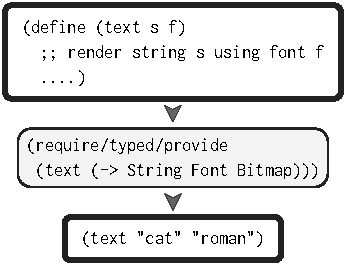
\includegraphics[trim=2.4000000000000004 2.4000000000000004 2.4000000000000004 2.4000000000000004]{pict.pdf}}}\end{FigureInside}\end{Centerfigure}

\Centertext{\Legend{\FigureTarget{\label{t:x28counter_x28x22figurex22_x22figx3adsx2dexamplex22x29x29}\textbf{\textbf{Figure}~\textbf{1}: }}{t:x28counter_x28x22figurex22_x22figx3adsx2dexamplex22x29x29}\textrm{Untyped library, typed interface, and untyped client}}}\end{Figure}

The question raised by this example is whether static types can catch the mistake
in the untyped client.
Deep and shallow types give opposite answers:


\noindent \begin{itemize}\atItemizeStart

\item Deep types enforce the typed interface with run{-}time obligations for both
the client and the library.
Because the client sends a string where the type expects a font object,
the client triggers a run{-}time type error.

\item Shallow types guarantee the local integrity of typed code, but nothing more.
The untyped client is allowed to send any input to the untyped \Scribtexttt{text}
function, including two strings, without causing a type{-}level error.\end{itemize}

From a theoretical perspective, shallow types satisfy a type soundness
property and nothing more\relax{~\citep{vss-popl-2017,gf-icfp-2018}}.
Soundness states that the type of an expression predicts the kinds of values
that evaluation can produce.
In typed code, these predictions are often specific and useful.
For example, an expression with a function type cannot evaluate to a number.
In untyped code, these predictions are trivial;
 soundness merely ensures a well{-}formed result.
A property that distinguishes deep types from shallow is
complete monitoring\relax{~\citep{dtf-esop-2012,gfd-oopsla-2019}}.
Semantics that satisfy complete monitoring enforce types as invariants
that all clients, typed or untyped, can rely on.

\begin{Figure}\begin{Centerfigure}\begin{FigureInside}\relax{ \newcommand{\bigicon}[1]{\scalebox{1.6}{\(#1\)}}\begin{tikzpicture}[tips=proper]

  \node (S) {\bigicon{\sS}};
  \node (D) [right of=S,xshift=1.4cm,yshift=8mm] {\bigicon{\sD}};
  \node (U) [right of=D,xshift=1.4cm,yshift=-8mm] {\bigicon{\sU}};

  \draw [>=latex,<->,very thick] (S) edge [bend left=7] node [above,xshift=-1mm] {\(\swrap\)} (D);
  %\draw [>=latex,<->] (D) edge [bend left=7] (S);

  \draw [>=latex,<->,very thick] (D) edge [bend left=7] node [above,xshift=2mm] {\(\swrap\)} (U);
  %\draw [>=latex,->] (U) edge [bend left=7] (D);

  \draw [>=latex,->,very thick] ([yshift=-0.5mm] S.east) edge [bend right=7] node [above,yshift=-1mm] {\(\snoop\)} ([yshift=-0.5mm] U.west);
  \draw [>=latex,->,very thick] ([yshift=-2mm] U.west) edge [bend left=7] node [below] {\(\sscan\)} ([yshift=-2mm] S.east);

  %\draw [->] (S) edge [loop, min distance=2mm,in=240,out=200,looseness=3] node [below] {\(\snoop\)} (S);
  %\draw [->] (D) edge [loop, min distance=2mm,in=110,out=70,looseness=3] node [above] {\(\snoop\)} (D);
  %\draw [->] (U) edge [loop, min distance=2mm,in=300,out=340,looseness=3] node [below] {\(\snoop\)} (U);

\end{tikzpicture}\vspace{-1ex} }\end{FigureInside}\end{Centerfigure}

\Centertext{\Legend{\FigureTarget{\label{t:x28counter_x28x22figurex22_x22figx3amodelx3abasex2dinteractionx22x29x29}\textbf{Figure}~\textbf{2}: }{t:x28counter_x28x22figurex22_x22figx3amodelx3abasex2dinteractionx22x29x29}\textrm{Outline for deep, shallow, and untyped interactions}}}\end{Figure}

\Ssubsubsection{Natural Semantics}{Natural Semantics}\label{t:x28part_x22Naturalx5fSemanticsx22x29}

One way to implement deep types is the Natural
semantics\relax{~\citep{tf-dls-2006,mf-toplas-2009,st-sfp-2006}}.\NoteBox{\NoteContent{Natural is a.k.a.
Guarded\relax{~\citep{vksb-dls-2014}}, Behavioral\relax{~\citep{clzv-ecoop-2018}}, and
Deep\relax{~\citep{tgpk-dls-2018}}.}}
Natural interprets types as contracts in a straightforward manner.\NoteBox{\NoteContent{Researchers are actively seeking improved variants of Natural\relax{~\citep{htf-hosc-2010,g-popl-2015,stw-pldi-2015,stw-jfp-2021,gct-popl-2016}}
and measuring the efficiency of implementations\relax{~\citep{fgsfs-oopsla-2018,kas-pldi-2019}}.
Theoretical results about Natural hold for these semantics{-}preserving variants as well.}}
For example, base types are enforced with predicate checks,
types for immutable values are enforced with first{-}order traversals,
and types for higher{-}order values such as arrays and functions are enforced with
higher{-}order \emph{wrapper} contracts.
Because each contract fully enforces a type, these contracts need only guard
the boundaries between typed and untyped code.
Within typed modules, code can run efficiently and employ type{-}directed
optimizations\relax{~\citep{tscff-pldi-2011}}.

\Ssubsubsection{Transient Semantics}{Transient Semantics}\label{t:x28part_x22Transientx5fSemanticsx22x29}

The Transient semantics is an implementation of shallow types that
does not require wrappers\relax{~\citep{vss-popl-2017}}.
Transient enforces types by injecting first{-}order
checks throughout typed pieces of code:
typed, public functions must check their inputs;
typed modules must check their untyped imports; and
typed expressions must check the results computed during a function call,
the elements extracted from a data structure, and the outcome of any
downcasts.
In figure~\hyperref[t:x28counter_x28x22figurex22_x22figx3amodelx3abasex2dinteractionx22x29x29]{\FigureRef{2}{t:x28counter_x28x22figurex22_x22figx3amodelx3abasex2dinteractionx22x29x29}}, these conditions imply one check:
the typed interface must check that \Scribtexttt{text} is a function.
In general, every line of typed code may add several
Transient checks, but each check is inexpensive.
By contrast to higher{-}order contracts, the checks
do not traverse values and do not impose allocation and indirection
costs.

\sectionNewpage

\Ssection{Model and Metatheory}{Model and Metatheory}\label{t:x28part_x22secx3amodelx22x29}

A normal gradual language allows for two styles of code, typed and untyped,
and uses run{-}time checks to enforce the claims made by static types.
Our model allows for three syntaxes:
deep{-}typed code, shallow{-}typed code, and untyped code.
Both deep and shallow code must satisfy the same type checker, which
validates conventional well{-}formedness properties.
Untyped code has fewer constraints.
Run{-}time checks enforce type claims at boundaries, but use different strategies
for deep and for shallow types.

Overall, the primary goal of the model is to test whether deep, shallow,
and untyped code can safely interoperate.
A secondary goal of the model is to outline an implementation.
For this reason, the three syntaxes compile to one kernel language
that can express a variety of standard run{-}time checks:
a \emph{wrap} term applies a contract,
a \emph{scan} term performs a first{-}order (predicate) check,
and a \emph{noop} term represents a boundary that any value may cross.
Figure~\hyperref[t:x28counter_x28x22figurex22_x22figx3amodelx3abasex2dinteractionx22x29x29]{\FigureRef{2}{t:x28counter_x28x22figurex22_x22figx3amodelx3abasex2dinteractionx22x29x29}} sketches the plan for applying these terms
at type boundaries in a way that protects deep and shallow code from untyped
values (including values that have passed through a typed context).

\Ssubsection{Three{-}Way Surface Syntax}{Three{-}Way Surface Syntax}\label{t:x28part_x22secx3amodelx3amodelx3asyntaxx22x29}

\begin{Figure}\begin{Centerfigure}\begin{FigureInside}\relax{\begin{langarray}
  \ssurface & \slangeq &
    \svar \mid \sint \mid \epair{\ssurface}{\ssurface} \mid
    \efun{\svar}{\ssurface}
    \mid \efun{\tann{\svar}{\stype}}{\ssurface}
    \mid \efun{\tann{\svar}{\tfloor{\stype}}}{\ssurface} \mid
  \\ & &
    \eunop{\,\ssurface} \mid \ebinop{\,\ssurface}{\ssurface} \mid
    \eappu{\ssurface}{\ssurface} \mid
    \emod{\slang}{\ssurface}
  \\
  \slang & \slangeq &
    \sD \mid \sS \mid \sU
  \\
  \stype & \slangeq &
    \tnat \mid \tint \mid \tpair{\stype}{\stype} \mid \tfun{\stype}{\stype}
  \\
  \stspec & \slangeq &
    \stype \mid \tfloor{\stype} \mid \tdyn
\end{langarray}}\end{FigureInside}\end{Centerfigure}

\Centertext{\Legend{\FigureTarget{\label{t:x28counter_x28x22figurex22_x22figx3amodelx3asurfacex22x29x29}\textbf{Figure}~\textbf{3}: }{t:x28counter_x28x22figurex22_x22figx3amodelx3asurfacex22x29x29}\textrm{Surface syntax}}}\end{Figure}

The surface syntax (figure~\hyperref[t:x28counter_x28x22figurex22_x22figx3amodelx3asurfacex22x29x29]{\FigureRef{3}{t:x28counter_x28x22figurex22_x22figx3amodelx3asurfacex22x29x29}}) equips a basic expression
language with optional type annotations and module boundaries.
Surface expressions \relax{$\ssurface$} consist of function applications (\relax{$\eappu{\ssurface}{\ssurface}$}),
 primitive operation applications (\relax{$\eunop{\ssurface}$}, \relax{$\ebinop{\ssurface}{\ssurface}$}),
 variables \relax{$\svar$},
 integers \relax{$\sint$},
 pairs \relax{$\epair{\ssurface}{\ssurface}$},
 and optionally{-}annotated functions.
An untyped function has no annotation (\relax{$\efun{\svar}{\ssurface}$}),
 a deep{-}typed function has a plain type annotation (\relax{$\efun{\tann{\svar}{\stype}}{\ssurface}$}),
 and a shallow{-}typed function has an underlined type annotation (\relax{$\efun{\tann{\svar}{\tfloor{\stype}}}{\ssurface}$}).
The underline is a syntactic hint that only the top{-}level shape of this type is
guaranteed at run{-}time.
Types \relax{$\stype$} express natural numbers (\relax{$\tnat$}),
 integers (\relax{$\tint$}),
 pairs (\relax{$\tpair{\stype}{\stype}$}),
 and functions (\relax{$\tfun{\stype}{\stype}$}).
Modules associate a label with an expression (\relax{$\emod{\slang}{\ssurface}$}).
The label \relax{$\slang$} is either \relax{$\sD$} for deep{-}typed code,
 \relax{$\sS$} for shallow{-}typed code, or \relax{$\sU$} for untyped code.
For example, the term \relax{$(\emod{\sD}{\ssurface_0})$} says that \relax{$\ssurface_0$}
is a deep{-}typed expression.
Any module expressions within \relax{$\ssurface_0$} are free to use any
typing style (\relax{$\sD$}, \relax{$\sS$}, or \relax{$\sU$}).

\Ssubsection{Three{-}Way Surface Typing}{Three{-}Way Surface Typing}\label{t:x28part_x22secx3amodelx3amodelx3atypesx22x29}

Deep and shallow code must satisfy strong (and equal) type constraints.
Untyped code is subject to a weaker constraint; namely, it cannot reference
variables that it did not bind.
These well{-}formedness conditions are spelled out in the typing judgment
of figure~\hyperref[t:x28counter_x28x22figurex22_x22figx3amodelx3asurfacex2dtypex22x29x29]{\FigureRef{4}{t:x28counter_x28x22figurex22_x22figx3amodelx3asurfacex2dtypex22x29x29}}, which relates a type environment
\relax{$\stypeenv$} and an expression \relax{$\ssurface$} to a result specification.
A result \relax{$\stspec$} is either a type \relax{$\stype$} for deep{-}typed code,
an underlined type \relax{$\tfloor{\stype}$} for shallow{-}typed code,
or the uni{-}type \relax{$\tdyn$} for untyped code.

With the exception of modules, the typing rules are standard for a basic
functional language.
Modules allow any kind of expression to appear within another.
For instance, an untyped expression may appear within a deep
expression provided that the untyped code is well{-}formed.
There are seven such rules to ensure that the module language (\relax{$\slang_0$})
matches the type of the subexpression (\relax{$\stspec_0$}); figure~\hyperref[t:x28counter_x28x22figurex22_x22figx3amodelx3asurfacex2dtypex22x29x29]{\FigureRef{4}{t:x28counter_x28x22figurex22_x22figx3amodelx3asurfacex2dtypex22x29x29}}
presents these rules as one template rule (in [brackets]) and a table.

Figure~\hyperref[t:x28counter_x28x22figurex22_x22figx3amodelx3asurfacex2dtypex22x29x29]{\FigureRef{4}{t:x28counter_x28x22figurex22_x22figx3amodelx3asurfacex2dtypex22x29x29}} also defines a subtyping judgment (\relax{$\ssubt$})
and a type{-}assignment for primitive operations (\relax{$\sDelta$}).
Subtyping declares that the natural numbers are a subset of the integers
and extends this covariantly to pairs and contra/co{-}variantly to
function domains/codomains.
The primitive operations are consequently overloaded to accept natural numbers or
integers.
The purpose of this basic subtyping judgment is not to sketch out a numeric tower\relax{~\citep{stff-padl-2012}},
but rather to show that an upcast (via subtyping) can weaken the run{-}time
checks that shallow code inserts.
Weakening may have serious pragmatic implications for gradual union,
intersection, and object types\relax{~\citep{cl-icfp-2017,tf-icfp-2010,aft-dls-2013,tsdtf-oopsla-2012,jd-popl-2017,tt-sas-2017}}.

\begin{Figure}\begin{Centerfigure}\begin{FigureInside}\relax{\lbl{\fbox{\(\stypeenv \sST \ssurface : \stspec\)}}{
\begin{mathpar}
  \inferrule*{
    \tann{\svar_0}{\stype_0} \in \stypeenv
  }{
    \stypeenv \sST \svar_0 : \stype_0
  }

  \inferrule*{
    \tann{\svar_0}{\tfloor{\stype_0}} \in \stypeenv
  }{
    \stypeenv \sST \svar_0 : \tfloor{\stype_0}
  }

  \inferrule*{
    \tann{\svar_0}{\tdyn} \in \stypeenv
  }{
    \stypeenv \sST \svar_0 : \tdyn
  }

%  \inferrule*{
%  }{
%    \stypeenv \sST \snat_0 : \tnat
%  }
%
%  \inferrule*{
%  }{
%    \stypeenv \sST \snat_0 : \tfloor{\tnat}
%  }
%
%  \inferrule*{
%  }{
%    \stypeenv \sST \snat_0 : \tdyn
%  }
%
%  \inferrule*{
%  }{
%    \stypeenv \sST \sint_0 : \tint
%  }
%
%  \inferrule*{
%  }{
%    \stypeenv \sST \sint_0 : \tfloor{\tint}
%  }
%
%  \inferrule*{
%    \stypeenv \sST \ssurface_0 : \tdyn
%    \\
%    \stypeenv \sST \ssurface_1 : \tdyn
%  }{
%    \stypeenv \sST \epair{\ssurface_0}{\ssurface_1} : \tdyn
%  }
%
%  \inferrule*{
%    \stypeenv \sST \ssurface_0 : \stype_0
%    \\
%    \stypeenv \sST \ssurface_1 : \stype_1
%  }{
%    \stypeenv \sST \epair{\ssurface_0}{\ssurface_1} : \tpair{\stype_0}{\stype_1}
%  }
%
%  \inferrule*{
%    \stypeenv \sST \ssurface_0 : \tfloor{\stype_0}
%    \\
%    \stypeenv \sST \ssurface_1 : \tfloor{\stype_1}
%  }{
%    \stypeenv \sST \epair{\ssurface_0}{\ssurface_1} : \tfloor{\tpair{\stype_0}{\stype_1}}
%  }
%
  \inferrule*{
    \fcons{\tann{\svar_0}{\stype_0}}{\stypeenv} \sST \sexpr_0 : \stype_1
  }{
    \stypeenv \sST \efun{\tann{\svar_0}{\stype_0}}{\sexpr_0} : \tfun{\stype_0}{\stype_1}
  }

  \inferrule*{
    \fcons{\tann{\svar_0}{\tfloor{\stype_0}}}{\stypeenv} \sST \sexpr_0 : \tfloor{\stype_1}
  }{
    \stypeenv \sST \efun{\tann{\svar_0}{\tfloor{\stype_0}}}{\sexpr_0} : \tfloor{\tfun{\stype_0}{\stype_1}}
  }

  \inferrule*{
    \fcons{\tann{\svar_0}{\tdyn}}{\stypeenv} \sST \sexpr_0 : \tdyn
  }{
    \stypeenv \sST \efun{\svar_0}{\sexpr_0} : \tdyn
  }
%
%  \inferrule*{
%    \stypeenv \sST \ssurface_0 : \tdyn
%    \\
%    \stypeenv \sST \ssurface_1 : \tdyn
%  }{
%    \stypeenv \sST \eappu{\ssurface_0}{\ssurface_1} : \tdyn
%  }
%
%  \inferrule*{
%    \stypeenv \sST \sexpr_0 : \tfun{\stype_0}{\stype_1}
%    \\
%    \stypeenv \sST \sexpr_1 : \stype_0
%  }{
%    \stypeenv \sST \eappu{\sexpr_0}{\sexpr_1} : \stype_1
%  }

  \inferrule*{
    \stypeenv \sST \sexpr_0 : \tfloor{\tfun{\stype_0}{\stype_1}}
    \\
    \stypeenv \sST \sexpr_1 : \tfloor{\stype_0}
  }{
    \stypeenv \sST \eappu{\sexpr_0}{\sexpr_1} : \tfloor{\stype_1}
  }

%  \inferrule*{
%    \stypeenv \sST \ssurface_0 : \tdyn
%  }{
%    \stypeenv \sST \eunop{\ssurface_0} : \tdyn
%  }
%
%  \inferrule*{
%    \stypeenv \sST \sexpr_0 : \stype_0
%    \\
%    \sDelta(\sunop, \stype_0)\!=\!\stype_1
%  }{
%    \stypeenv \sST \eunop{\sexpr_0} : \stype_1
%  }
%
%  \inferrule*{
%    \stypeenv \sST \sexpr_0 : \tfloor{\stype_0}
%    \\
%    \sDelta(\sunop, \stype_0) = \stype_1
%  }{
%    \stypeenv \sST \eunop{\sexpr_0} : \tfloor{\stype_1}
%  }
%
%  \inferrule*{
%    \stypeenv \sST \ssurface_0 : \tdyn
%    \\
%    \stypeenv \sST \ssurface_1 : \tdyn
%  }{
%    \stypeenv \sST \ebinop{\ssurface_0}{\ssurface_1} : \tdyn
%  }
%
%  \inferrule*{
%    \stypeenv \sST \sexpr_0 : \stype_0
%    \\
%    \stypeenv \sST \sexpr_1 : \stype_1
%    \\\\
%    \sDelta(\sbinop, \stype_0, \stype_1) = \stype_2
%  }{
%    \stypeenv \sST \ebinop{\sexpr_0}{\sexpr_1} : \stype_2
%  }
%
%  \inferrule*{
%    \stypeenv \sST \sexpr_0 : \tfloor{\stype_0}
%    \\
%    \stypeenv \sST \sexpr_1 : \tfloor{\stype_1}
%    \\\\
%    \sDelta(\sbinop, \stype_0, \stype_1) = \stype_2
%  }{
%    \stypeenv \sST \ebinop{\sexpr_0}{\sexpr_1} : \tfloor{\stype_2}
%  }

  \inferrule*{
    \stypeenv \sST \sexpr_0 : \stype_0
    \\
    \fsubt{\stype_0}{\stype_1}
  }{
    \stypeenv \sST \sexpr_0 : \stype_1
  }

  \inferrule*{
    \stypeenv \sST \sexpr_0 : \tfloor{\stype_0}
    \\
    \fsubt{\stype_0}{\stype_1}
  }{
    \stypeenv \sST \sexpr_0 : \tfloor{\stype_1}
  }

%  \inferrule*{
%    \stypeenv \sST \sexpr_0 : \tdyn
%  }{
%    \stypeenv \sST \emodule{\sulang}{\sexpr_0} : \tdyn
%  }
%
%  \inferrule*{
%    \stypeenv \sST \sexpr_0 : \stype_0
%  }{
%    \stypeenv \sST \emodule{\sdlang}{\sexpr_0} : \tdyn
%  }
%
%  \inferrule*{
%    \stypeenv \sST \sexpr_0 : \tfloor{\stype_0}
%  }{
%    \stypeenv \sST \emodule{\sslang}{\sexpr_0} : \tdyn
%  }
%
%  \inferrule*{
%    \stypeenv \sST \sexpr_0 : \tdyn
%  }{
%    \stypeenv \sST \emodule{\sulang}{\sexpr_0} : \stype_0
%  }
%
%  \inferrule*{
%    \stypeenv \sST \sexpr_0 : \stype_0
%  }{
%    \stypeenv \sST \emodule{\sdlang}{\sexpr_0} : \stype_0
%  }
%
%  \inferrule*{
%    \stypeenv \sST \sexpr_0 : \tfloor{\stype_0}
%  }{
%    \stypeenv \sST \emodule{\sslang}{\sexpr_0} : \stype_0
%  }
%
%  \inferrule*{
%    \stypeenv \sST \sexpr_0 : \tdyn
%  }{
%    \stypeenv \sST \emodule{\sulang}{\sexpr_0} : \tfloor{\stype_0}
%  }
%
%  \inferrule*{
%    \stypeenv \sST \sexpr_0 : \stype_0
%  }{
%    \stypeenv \sST \emodule{\sdlang}{\sexpr_0} : \tfloor{\stype_0}
%  }
%
%  \inferrule*{
%    \stypeenv \sST \sexpr_0 : \tfloor{\stype_0}
%  }{
%    \stypeenv \sST \emodule{\sslang}{\sexpr_0} : \tfloor{\stype_0}
%  }
\end{mathpar}

\medskip
\begin{tabular}{l@{\qquad}l}
\(\left[
  \inferrule*{
    \stypeenv \sST \sexpr_0 : \stspec_0
  }{
    \stypeenv \sST \emodule{\slang_0}{\sexpr_0} : \stspec_1
  }
\right]\) &
\(\begin{array}{llll}
  \slang_0 & \stspec_0 & \stspec_1 \\\hline
  \sD & \stype_0 & \stype_0 \\
  \sD & \stype_0 & \tfloor{\stype_0} \\
  \sD & \stype_0 & \tdyn \\
  \sS & \tfloor{\stype_0} & \stype_0 \\
  \sS & \tfloor{\stype_0} & \tfloor{\stype_0} \\
  \sS & \tfloor{\stype_0} & \tdyn \\
  \sU & \tdyn & \stspec_1
\end{array}\) \end{tabular}
}

\medskip
\begin{minipage}[t]{0.48\columnwidth}
\lbl{\fbox{$\fsubt{\stype}{\stype}$}}{\begin{mathpar}
\vspace{-2ex}
  \inferrule*{
  }{
    \fsubt{\tnat}{\tint}
  }

\vspace{-2ex}
  \inferrule*{
    \fsubt{\stype_0}{\stype_2}
    \\
    \fsubt{\stype_1}{\stype_3}
  }{
    \fsubt{\tpair{\stype_0}{\stype_1}}{\tpair{\stype_2}{\stype_3}}
  }

\vspace{-0ex}
  \inferrule*{
    \fsubt{\stype_2}{\stype_0}
    \\
    \fsubt{\stype_1}{\stype_3}
  }{
    \fsubt{\tfun{\stype_0}{\stype_1}}{\tfun{\stype_2}{\stype_3}}
  }
\end{mathpar}}
\end{minipage}\begin{minipage}[t]{0.52\columnwidth}
\lbl{\fbox{$\sDelta : \ffun{\tpair{\sunop\,}{\,\stype}}{\stype}$}}{
  \begin{langarray}
    \sDelta(\sfst, \tpair{\stype_0}{\stype_1}) & \feq & \stype_0
  \\
    \sDelta(\ssnd, \tpair{\stype_0}{\stype_1}) & \feq & \stype_1
  \end{langarray}
}\medskip

\lbl{\fbox{$\sDelta : \ffun{\tpair{\sbinop\,}{\tpair{\,\stype\,}{\,\stype}}}{\stype}$}}{
  \begin{langarray}
    \sDelta(\ssum, \tnat, \tnat) & \feq & \tnat
  \\
    \sDelta(\ssum, \tint, \tint) & \feq & \tint
  \\
    \sDelta(\squotient, \tnat, \tnat) & \feq & \tnat
  \\
    \sDelta(\squotient, \tint, \tint) & \feq & \tint
  \end{langarray}
}
\end{minipage}
}\end{FigureInside}\end{Centerfigure}

\Centertext{\Legend{\FigureTarget{\label{t:x28counter_x28x22figurex22_x22figx3amodelx3asurfacex2dtypex22x29x29}\textbf{Figure}~\textbf{4}: }{t:x28counter_x28x22figurex22_x22figx3amodelx3asurfacex2dtypex22x29x29}\textrm{Surface typing (selected rules), subtyping, and types for primitive operations}}}\end{Figure}

\Ssubsection{Common Evaluation Syntax}{Common Evaluation Syntax}\label{t:x28part_x22secx3amodelx3amodelx3aevalx2dsyntaxx22x29}

Evaluation expressions \relax{$\sexpr$} consist of variables, values, primitive
applications, function applications, errors, and boundary terms.
Unlike the surface syntax, there are no module terms.
Instead, the three \emph{boundary terms} describe run{-}time checks.
A wrap boundary asks for the full enforcement of a type, either with a comprehensive first{-}order
check or a higher{-}order wrapper.
A scan boundary asks for a first{-}order type{-}shape (\relax{$\sshape$}) check.
A noop boundary asks for no check.

Values and errors represent the possible results of an evaluation.
The values are integers, pairs, functions, and guard wrappers.
A guard wrapper \relax{$(\emon{(\tfun{\stype_0}{\stype_1})}{\svalue_0})$} provides
type{-}restricted access to a function.
Shallow{-}typed functions have a shape annotation and a \relax{$\sscan$} tag in
the evaluation syntax (\relax{$\esfun{\svar}{\sshape}{\sexpr}$})
to suggest that such functions must validate the shape of their input at run{-}time.
Errors may arise from either a failed check at wrap boundary (\relax{$\swraperror$}),
a failed check at a scan boundary (\relax{$\sscanerror$}), a division by zero
(\relax{$\sdivzeroerror$}), or a malformed untyped expression (\relax{$\stagerror$}).

\begin{Figure}\begin{Centerfigure}\begin{FigureInside}\relax{\begin{langarray}
  \sexpr & \slangeq &
    \svar \mid \svalue \mid \epair{\sexpr}{\sexpr}
    \mid \eunop{\sexpr} \mid
    \ebinop{\sexpr}{\sexpr} \mid \eappu{\sexpr}{\sexpr} \mid
  \\ & &
    \serror
    \mid \ewrap{\stype}{\sexpr}
    \mid \escan{\sshape}{\sexpr}
    \mid \enoop{\sexpr}
  \\
  \svalue & \slangeq &
    \sint \mid \epair{\svalue}{\svalue}
    \mid \efun{\svar}{\sexpr}
    \mid \efun{\tann{\svar}{\stype}}{\sexpr}
    \mid \esfun{\svar}{\sshape}{\sexpr} \mid
  \\ & &
    \emon{(\tfun{\stype}{\stype})}{\svalue}
  \\
  \sshape & \slangeq &
    \knat \mid \kint \mid \kpair \mid \kfun \mid \kany
  \\
  \serror & \slangeq &
    \swraperror \mid \sscanerror \mid \sdivzeroerror \mid \stagerror
  \\
  \sctx & \slangeq &
    \sctxhole \mid \eunop{\sctx} \mid \ebinop{\sctx}{\sexpr} \mid \ebinop{\svalue}{\sctx}\
    \mid \epair{\sctx}{\sexpr} \mid \epair{\svalue}{\sctx}
    \mid\!\!\!\!
  \\ & &
    \eappu{\sctx}{\sexpr} \mid \eappu{\svalue}{\sctx} \mid \enoop{\sctx} \mid \escan{\sshape}{\sctx} \mid \ewrap{\stype}{\sctx}
\end{langarray}}\end{FigureInside}\end{Centerfigure}

\Centertext{\Legend{\FigureTarget{\label{t:x28counter_x28x22figurex22_x22figx3amodelx3aevalx2dsyntaxx22x29x29}\textbf{Figure}~\textbf{5}: }{t:x28counter_x28x22figurex22_x22figx3amodelx3aevalx2dsyntaxx22x29x29}\textrm{Evaluation syntax}}}\end{Figure}

\Ssubsection{Three{-}Way Evaluation Typing}{Three{-}Way Evaluation Typing}\label{t:x28part_x22secx3amodelx3amodelx3aevalx2dtypesx22x29}

The evaluation syntax comes with three typing judgments that describe the
invariants of deep, shallow, and untyped code.
The deep typing judgment (\relax{$\sWTD$}) validates full types,
the shallow judgment (\relax{$\sWTS$}) checks top{-}level type shapes,
and the untyped judgment (\relax{$\sWTU$}) checks that all variables
are bound.

Both the deep and untyped rules are similar to the corresponding
surface{-}language rules because they support equally{-}strong conclusions
(full types and the uni{-}type).
The shallow judgment is different because it validates type
shapes instead of full types.
When inspecting a pair, for example, the shallow judgment concludes with the \relax{$\kpair$}
shape no matter what shapes the elements have.
Consequently, a pair elimination form such as \relax{$(\efstu{\svar_0})$} has the
\relax{$\kany$} shape because the pair may contain any sort of value.
Similar comments apply to functions and applications.
Thus if a program expects a certain shape from a pair element or a
function call, then the program must use a \relax{$\sscan$} term to
confirm the expectation.

\begin{Figure}\begin{Centerfigure}\begin{FigureInside}\relax{\lbl{\fbox{\(\stypeenv \sWTT \sexpr : \stype\)}}{
\begin{mathpar}
  \inferrule*{
    \tann{\svar_0}{\stype_0} \in \stypeenv
  }{
    \stypeenv \sWTT \svar_0 : \stype_0
  }

%  \inferrule*{
%  }{
%    \stypeenv \sWTT \snat_0 : \tnat
%  }
%
%  \inferrule*{
%  }{
%    \stypeenv \sWTT \sint_0 : \tint
%  }
%
%  \inferrule*{
%    \stypeenv \sWTT \sexpr_0 : \stype_0
%    \\
%    \stypeenv \sWTT \sexpr_1 : \stype_1
%  }{
%    \stypeenv \sWTT \epair{\sexpr_0}{\sexpr_1} : \tpair{\stype_0}{\stype_1}
%  }
%
  \inferrule*{
    \fcons{\tann{\svar_0}{\stype_0}}{\stypeenv} \sWTT \sexpr_0 : \stype_1
  }{
    \stypeenv \sWTT \efun{\tann{\svar_0}{\stype_0}}{\sexpr_0} : \tfun{\stype_0}{\stype_1}
  }

  \inferrule*{
    \stypeenv \sWTU \svalue_0 : \tdyn
  }{
    \stypeenv \sWTT \emon{\stype_0}{\svalue_0} : \stype_0
  }

  \inferrule*{
    \stypeenv \sWTS \svalue_0 : \sshape_0
  }{
    \stypeenv \sWTT \emon{\stype_0}{\svalue_0} : \stype_0
  }

%  \inferrule*{
%    \stypeenv \sWTT \sexpr_0 : \stype_0
%    \\\\
%    \sDelta(\sunop, \stype_0) = \stype_1
%  }{
%    \stypeenv \sWTT \eunop{\sexpr_0} : \stype_1
%  }
%
%  \inferrule*{
%    \stypeenv \sWTT \sexpr_0 : \stype_0
%    \\
%    \stypeenv \sWTT \sexpr_1 : \stype_1
%    \\\\
%    \sDelta(\sbinop, \stype_0, \stype_1) = \stype_2
%  }{
%    \stypeenv \sWTT \ebinop{\sexpr_0}{\sexpr_1} : \stype_2
%  }
%
  \inferrule*{
    \stypeenv \sWTT \sexpr_0 : \tfun{\stype_0}{\stype_1}
    \\
    \stypeenv \sWTT \sexpr_1 : \stype_0
  }{
    \stypeenv \sWTT \eappu{\sexpr_0}{\sexpr_1} : \stype_1
  }

  \inferrule*{
    \stypeenv \sWTT \sexpr_0 : \stype_0
  }{
    \stypeenv \sWTT \enoop{\sexpr_0} : \stype_0
  }

  \inferrule*{
    \stypeenv \sWTU \sexpr_0 : \tdyn
  }{
    \stypeenv \sWTT \ewrap{\stype_0}{\sexpr_0} : \stype_0
  }

  \inferrule*{
    \stypeenv \sWTS \sexpr_0 : \sshape_0
  }{
    \stypeenv \sWTT \ewrap{\stype_0}{\sexpr_0} : \stype_0
  }

%  \inferrule*{
%    \stypeenv \sWTT \sexpr_0 : \stype_0
%    \\
%    \fsubt{\stype_0}{\stype_1}
%  }{
%    \stypeenv \sWTT \sexpr_0 : \stype_1
%  }
%
%  \inferrule*{
%  }{
%    \stypeenv \sWTT \serror : \stype_0
%  }
\end{mathpar}
}}\end{FigureInside}\end{Centerfigure}

\Centertext{\Legend{\FigureTarget{\label{t:x28counter_x28x22figurex22_x22figx3amodelx3adeepx2dtypex22x29x29}\textbf{Figure}~\textbf{6}: }{t:x28counter_x28x22figurex22_x22figx3amodelx3adeepx2dtypex22x29x29}\textrm{Deep typing judgment (selected rules)}}}\end{Figure}

\begin{Figure}\begin{Centerfigure}\begin{FigureInside}\relax{\lbl{\fbox{\(\stypeenv \sWTS \sexpr : \sshape\)}}{
\begin{mathpar}
  \inferrule*{
    \tann{\svar_0}{\sshape_0} \in \stypeenv
  }{
    \stypeenv \sWTS \svar_0 : \sshape_0
  }

%  \inferrule*{
%  }{
%    \stypeenv \sWTS \snat_0 : \tnat
%  }
%
%  \inferrule*{
%  }{
%    \stypeenv \sWTS \sint_0 : \tint
%  }
%
%  \inferrule*{
%    \stypeenv \sWTS \sexpr_0 : \sshape_0
%    \\
%    \stypeenv \sWTS \sexpr_1 : \sshape_1
%  }{
%    \stypeenv \sWTS \epair{\sexpr_0}{\sexpr_1} : \kpair
%  }
%
  \inferrule*{
    \fcons{\tann{\svar_0}{\tdyn}}{\stypeenv} \sWTU \sexpr_0 : \tdyn
  }{
    \stypeenv \sWTS \efun{\svar_0}{\sexpr_0} : \kfun
  }

  \inferrule*{
    \fcons{\tann{\svar_0}{\sshape_0}}{\stypeenv} \sWTS \sexpr_0 : \sshape_1
  }{
    \stypeenv \sWTS \esfun{\svar_0}{\sshape_0}{\sexpr_0} : \kfun
  }

  \inferrule*{
    \stypeenv \sWTT \svalue_0 : \stype_0
  }{
    \stypeenv \sWTS \emon{\stype_0}{\svalue_0} : \kfun
  }

%  \inferrule*{
%    \stypeenv \sWTS \sexpr_0 : \sshape_0
%  }{
%    \stypeenv \sWTS \eunop{\sexpr_0} : \kany
%  }
%
%  \inferrule*{
%    \stypeenv \sWTS \sexpr_0 : \sshape_0
%    \\
%    \stypeenv \sWTS \sexpr_1 : \sshape_1
%    \\
%    \sDelta(\sbinop, \sshape_0, \sshape_1) = \sshape_2
%  }{
%    \stypeenv \sWTS \ebinop{\sexpr_0}{\sexpr_1} : \sshape_2
%  }
%
  \inferrule*{
    \stypeenv \sWTS \sexpr_0 : \kfun
    \\
    \stypeenv \sWTS \sexpr_1 : \sshape_0
  }{
    \stypeenv \sWTS \eappu{\sexpr_0}{\sexpr_1} : \kany
  }

  \inferrule*{
    \stypeenv \sWTS \sexpr_0 : \sshape_0
  }{
    \stypeenv \sWTS \enoop{\sexpr_0} : \sshape_0
  }

  \inferrule*{
    %% why need this???
    %% 2021-04-25 : because no way to check 'any' ... it should be a scan ... let's fix that
    \stypeenv \sWTU \sexpr_0 : \tdyn
  }{
    \stypeenv \sWTS \enoop{\sexpr_0} : \kany
  }

  \inferrule*{
    \stypeenv \sWTU \sexpr_0 : \tdyn
  }{
    \stypeenv \sWTS \escan{\sshape_0}{\sexpr_0} : \sshape_0
  }

  \inferrule*{
    \stypeenv \sWTS \sexpr_0 : \sshape_1
  }{
    \stypeenv \sWTS \escan{\sshape_0}{\sexpr_0} : \sshape_0
  }

  \inferrule*{
    \stypeenv \sWTT \sexpr_0 : \stype_0
    \\
    \fshape{\stype_0} = \sshape_0
  }{
    \stypeenv \sWTS \ewrap{\stype_0}{\sexpr_0} : \sshape_0
  }

%  \inferrule*{
%    \stypeenv \sWTS \sexpr_0 : \sshape_0
%    \\
%    \fsubt{\sshape_0}{\sshape_1}
%  }{
%    \stypeenv \sWTS \sexpr_0 : \sshape_1
%  }
%
%  \inferrule*{
%  }{
%    \stypeenv \sWTS \serror : \sshape_0
%  }
\end{mathpar}
}

\medskip
\lbl{\fbox{$\fsubt{\sshape}{\sshape}$}}{\vspace{-0.6cm}\begin{mathpar}
  \inferrule*{
  }{
    \fsubt{\knat}{\kint}
  }

  \inferrule*{
  }{
    \fsubt{\sshape_0}{\kany}
  }
\end{mathpar}}

\medskip
\lbl{\fbox{$\sshapecheck : \ffun{\stype}{\sshape}$}}{
\begin{tabular}{ll}
  \begin{langarray}
    \fshape{\tnat} & \feq & \knat
  \\
    \fshape{\tint} & \feq & \kint
  \end{langarray} &
  \begin{langarray}
    \fshape{\tpair{\stype_0}{\stype_1}} & \feq & \kpair
  \\
    \fshape{\tfun{\stype_0}{\stype_1}} & \feq & \kfun
  \end{langarray}
\end{tabular}}}\end{FigureInside}\end{Centerfigure}

\Centertext{\Legend{\FigureTarget{\label{t:x28counter_x28x22figurex22_x22figx3amodelx3ashallowx2dtypex22x29x29}\textbf{Figure}~\textbf{7}: }{t:x28counter_x28x22figurex22_x22figx3amodelx3ashallowx2dtypex22x29x29}\textrm{Shallow typing (selected rules), subtyping, and type{-}to{-}shape metafunction}}}\end{Figure}

\begin{Figure}\begin{Centerfigure}\begin{FigureInside}\relax{\lbl{\fbox{\(\stypeenv \sWTU \sexpr : \tdyn\)}}{\begin{mathpar}
  \inferrule*{
    \tann{\svar_0}{\tdyn} \in \stypeenv
  }{
    \stypeenv \sWTU \svar_0 : \tdyn
  }

%  \inferrule*{
%  }{
%    \stypeenv \sWTU \sint_0 : \tdyn
%  }
%
%  \inferrule*{
%    \stypeenv \sWTU \sexpr_0 : \tdyn
%    \\
%    \stypeenv \sWTU \sexpr_1 : \tdyn
%  }{
%    \stypeenv \sWTU \epair{\sexpr_0}{\sexpr_1} : \tdyn
%  }
%
  \inferrule*{
    \fcons{\tann{\svar_0}{\tdyn}}{\stypeenv} \sWTU \sexpr_0 : \tdyn
  }{
    \stypeenv \sWTU \efun{\svar_0}{\sexpr_0} : \tdyn
  }

  \inferrule*{
    \fcons{\tann{\svar_0}{\sshape_0}}{\stypeenv} \sWTS \sexpr_0 : \sshape_1
  }{
    \stypeenv \sWTU \esfun{\svar_0}{\sshape_0}{\sexpr_0} : \tdyn
  }

  \inferrule*{
    \stypeenv \sWTT \svalue_0 : \stype_0
  }{
    \stypeenv \sWTU \emon{\stype_0}{\svalue_0} : \tdyn
  }

%  \inferrule*{
%    \stypeenv \sWTU \sexpr_0 : \tdyn
%  }{
%    \stypeenv \sWTU \eunop{\sexpr_0} : \tdyn
%  }
%
%  \inferrule*{
%    \stypeenv \sWTU \sexpr_0 : \tdyn
%    \\
%    \stypeenv \sWTU \sexpr_1 : \tdyn
%  }{
%    \stypeenv \sWTU \ebinop{\sexpr_0}{\sexpr_1} : \tdyn
%  }
%
  \inferrule*{
    \stypeenv \sWTU \sexpr_0 : \tdyn
    \\
    \stypeenv \sWTU \sexpr_1 : \tdyn
  }{
    \stypeenv \sWTU \eappu{\sexpr_0}{\sexpr_1} : \tdyn
  }

%  \inferrule*{
%    \stypeenv \sWTU \sexpr_0 : \tdyn
%  }{
%    \stypeenv \sWTU \enoop{\sexpr_0} : \tdyn
%  }
%
%  \inferrule*{
%    \stypeenv \sWTS \sexpr_0 : \sshape_0
%  }{
%    \stypeenv \sWTU \enoop{\sexpr_0} : \tdyn
%  }
%
%  \inferrule*{
%    \stypeenv \sWTU \sexpr_0 : \tdyn
%  }{
%    \stypeenv \sWTU \escan{\sshape_0}{\sexpr_0} : \tdyn
%  }
%
%  \inferrule*{
%    \stypeenv \sWTS \sexpr_0 : \sshape_1
%  }{
%    \stypeenv \sWTU \escan{\sshape_0}{\sexpr_0} : \tdyn
%  }
%
  \inferrule*{
    \stypeenv \sWTT \sexpr_0 : \stype_0
  }{
    \stypeenv \sWTU \ewrap{\stype_0}{\sexpr_0} : \tdyn
  }
%
%  \inferrule*{
%  }{
%    \stypeenv \sWTU \serror : \tdyn
%  }
\end{mathpar}
}}\end{FigureInside}\end{Centerfigure}

\Centertext{\Legend{\FigureTarget{\label{t:x28counter_x28x22figurex22_x22figx3amodelx3auntypedx2dtypex22x29x29}\textbf{Figure}~\textbf{8}: }{t:x28counter_x28x22figurex22_x22figx3amodelx3auntypedx2dtypex22x29x29}\textrm{Untyped typing judgment (selected rules)}}}\end{Figure}

\begin{Figure}\begin{Centerfigure}\begin{FigureInside}\relax{\lbl{\fbox{\(\stypeenv \sST \ssurface : \stspec \scompile \sexpr\)}}{\begin{mathpar}
  \inferrule*{
  }{
    \stypeenv\!\sST\!\svar_0\!:\!\stspec_0\!\scompile\!\svar_0
  }

%  \inferrule*{
%  }{
%    \stypeenv \sST \svar_0 : \stype_0 \scompile \svar_0
%  }
%
%  \inferrule*{
%  }{
%    \stypeenv \sST \svar_0 : \tfloor{\stype_0} \scompile \svar_0
%  }
%
%  \inferrule*{
%  }{
%    \stypeenv \sST \sint_0 : \tdyn \scompile \sint_0
%  }
%
%  \inferrule*{
%  }{
%    \stypeenv \sST \sint_0 : \stype_0 \scompile \sint_0
%  }
%
%  \inferrule*{
%  }{
%    \stypeenv \sST \sint_0 : \tfloor{\stype_0} \scompile \sint_0
%  }
%
%  \inferrule*{
%    \stypeenv \sST \sexpr_0 : \tdyn \scompile \sexpr_2
%    \\\\
%    \stypeenv \sST \sexpr_1 : \tdyn \scompile \sexpr_3
%  }{
%    \stypeenv \sST \epair{\sexpr_0}{\sexpr_1} : \tdyn \scompile \epair{\sexpr_2}{\sexpr_3}
%  }
%
%  \inferrule*{
%    \stypeenv \sST \sexpr_0 : \stype_0 \scompile \sexpr_2
%    \\\\
%    \stypeenv \sST \sexpr_1 : \stype_1 \scompile \sexpr_3
%  }{
%    \stypeenv \sST \epair{\sexpr_0}{\sexpr_1} : \tpair{\stype_0}{\stype_1} \scompile \epair{\sexpr_2}{\sexpr_3}
%  }
%
%  \inferrule*{
%    \stypeenv \sST \sexpr_0 : \tfloor{\stype_0} \scompile \sexpr_2
%    \\\\
%    \stypeenv \sST \sexpr_1 : \tfloor{\stype_1} \scompile \sexpr_3
%  }{
%    \stypeenv \sST \epair{\sexpr_0}{\sexpr_1} : \tfloor{\tpair{\stype_0}{\stype_1}} \scompile \epair{\sexpr_2}{\sexpr_3}
%  }
%
  \inferrule*{
    \fcons{\tann{\svar_0}{\stype_0}}{\stypeenv} \sST \sexpr_0 : \stype_1 \scompile \sexpr_1
  }{
    \stypeenv\!\sST\!\efun{\tann{\svar_0}{\stype_0}}{\sexpr_0}\!:\!\tfun{\stype_0}{\stype_1}\!\scompile\!\efun{\tann{\svar_0}{\stype_0}}{\sexpr_1}
  }

  \inferrule*{
    \fcons{\tann{\svar_0}{\tfloor{\stype_0}}}{\stypeenv} \sST \sexpr_0 : \tfloor{\stype_1} \scompile \sexpr_1
    \\
    \fshape{\stype_0} = \sshape_0
  }{
    \stypeenv \sST \efun{\tann{\svar_0}{\tfloor{\stype_0}}}{\sexpr_0} : \tfloor{\tfun{\stype_0}{\stype_1}} \scompile \esfun{\svar_0}{\sshape_0}{\sexpr_1}
  }

%  \inferrule*{
%    \fcons{\tann{\svar_0}{\tdyn}}{\stypeenv} \sST \sexpr_0 : \tdyn \scompile \sexpr_1
%  }{
%    \stypeenv \sST \efun{\svar_0}{\sexpr_0} : \tdyn \scompile \efun{\svar_0}{\sexpr_1}
%  }
%
  \inferrule*{
    \stypeenv \sST \sexpr_0 : \tfun{\stype_1}{\stype_0} \scompile \sexpr_2
    \\
    \stypeenv \sST \sexpr_1 : \stype_1 \scompile \sexpr_3
  }{
    \stypeenv \sST \eappu{\sexpr_0}{\sexpr_1} : \stype_0 \scompile \eappu{\sexpr_2}{\sexpr_3}
  }

  \inferrule*{
    \stypeenv \sST \sexpr_0 : \tfloor{\tfun{\stype_1}{\stype_0}} \scompile \sexpr_2
    \\
    \stypeenv \sST \sexpr_1 : \tfloor{\stype_1} \scompile \sexpr_3
    \\
    \fshape{\stype_0} = \sshape_0
  }{
    \stypeenv \sST \eappu{\sexpr_0}{\sexpr_1} : \tfloor{\stype_0} \scompile \escan{\sshape_0}{(\eappu{\sexpr_2}{\sexpr_3})}
  }
%
%  \inferrule*{
%    \stypeenv \sST \sexpr_0 : \tdyn \scompile \sexpr_2
%    \\
%    \stypeenv \sST \sexpr_1 : \tdyn \scompile \sexpr_3
%  }{
%    \stypeenv \sST \eappu{\sexpr_0}{\sexpr_1} : \tdyn \scompile \eappu{\sexpr_2}{\sexpr_3}
%  }
\end{mathpar}

\medskip
\begin{tabular}[t]{l@{~~}l}
\!\!\!\!\(\left[
  \inferrule*{
    \stypeenv \sST \sexpr_0 : \stspec_0 \scompile \sexpr_1
  }{
    \stypeenv\!\sST\!\emodule{\slang_0}{\sexpr_0}\!:\!\stspec_1\!\scompile\!\sexpr_2
  }
\right]\) &
\(\begin{array}{llll}
  \slang_0 & \stspec_0 & \stspec_1 & \scompile \sexpr_2 \!\! \\\hline
  \sD & \stype_0 & \tdyn & \ewrap{\stype_0}{\sexpr_1} \!\! \\
  \sS & \tfloor{\stype_0} & \stype_0 & \ewrap{\stype_0}{\sexpr_1} \!\! \\
  \sU & \tdyn & \stype_0 & \ewrap{\stype_0}{\sexpr_1} \!\! \\
  \sD & \stype_0 & \tfloor{\stype_0} & \ewrap{\stype_0}{\sexpr_1} \!\! \\
  \sS & \tfloor{\stype_0} & \tdyn & \enoop{\sexpr_1} \!\! \\
  \sU & \tdyn & \tfloor{\stype_0} & \escan{\sshape_0}{\sexpr_1} \!\!
\end{array}\)
\\ & \qquad\hbox{where \(\sshape_0 = \fshape{\stype_0}\)}

%  \sU & \tdyn & \tdyn & \enoop{\sexpr_1} \\
%  \sD & \stype_0 & \stype_0 & \enoop{\sexpr_1} \\
%  \sS & \tfloor{\stype_0} & \tfloor{\stype_0} & \enoop{\sexpr_1} \\
\end{tabular}

}}\end{FigureInside}\end{Centerfigure}

\Centertext{\Legend{\FigureTarget{\label{t:x28counter_x28x22figurex22_x22figx3amodelx3acompletion1x22x29x29}\textbf{Figure}~\textbf{9}: }{t:x28counter_x28x22figurex22_x22figx3amodelx3acompletion1x22x29x29}\textrm{Surface{-}to{-}evaluation compilation (selected rules)}}}\end{Figure}

\Ssubsection{Compilation from Surface to Evaluation}{Compilation from Surface to Evaluation}\label{t:x28part_x22secx3amodelx3amodelx3acompletionx22x29}

A compilation pass maps surface terms with modules to evaluation{-}language
terms with run{-}time checks.
The goal of the inserted checks is to ensure that well{-}typed surface
expressions are well{-}typed in the evaluation syntax.


\noindent \begin{itemize}\atItemizeStart

\item In deep{-}typed code, all module boundaries to non{-}deep code
become wrap checks. Compilation inserts no other checks.

\item In shallow code, deep boundaries become wrap checks
and untyped boundaries become scan checks.
Extra scan checks protect typed code (e.g., from pairs).

\item In untyped code, boundaries to deep modules become wrap checks
and boundaries to shallow modules become scan checks.
There are no other checks.\end{itemize}

\noindent \noindent{}The rules in figure~\hyperref[t:x28counter_x28x22figurex22_x22figx3amodelx3acompletion1x22x29x29]{\FigureRef{9}{t:x28counter_x28x22figurex22_x22figx3amodelx3acompletion1x22x29x29}}
present selected details of compilation.
Variables compile to themselves.
Functions in deep (and untyped) code simply recur on the
function body and compile to a new function.
Functions in shallow code add a scan tag to their argument to indicate
the need for a domain check, because untyped code can potentially invoke these functions.
Applications in deep (and untyped) code recur on their subexpressions.
Applications in shallow code insert an additional scan check to validate
the result.
Pair elimination forms (\relax{$\sfst$}, \relax{$\ssnd$}) use scans in a similar way.
Finally, one template rule and a table represent six rules for module boundaries.
These rules correspond to arrows in figure~\hyperref[t:x28counter_x28x22figurex22_x22figx3amodelx3abasex2dinteractionx22x29x29]{\FigureRef{2}{t:x28counter_x28x22figurex22_x22figx3amodelx3abasex2dinteractionx22x29x29}}.

\paragraph{Example}

The three{-}module program from figure~\hyperref[t:x28counter_x28x22figurex22_x22figx3adsx2dexamplex22x29x29]{\FigureRef{1}{t:x28counter_x28x22figurex22_x22figx3adsx2dexamplex22x29x29}} can be encoded with
shallow types roughly as follows:

\relax{\(
\begin{array}{l}
  \elet{\svar_0}{\emodule{\sslang}{(\emodule{\sulang}{(\efun{\svar_0\,\svar_1}{\texttt{\_}})})}}{}
  \\ \quad\eappu{\svar_0}{\texttt{`cat'}\,\texttt{`roman'}}
  \end{array}
\)}

\noindent{}Compilation yields a term with one \relax{$\sscan$} check:

\relax{\(
\begin{array}{l}
  \elet{\svar_0}{\enoop{(\escan{\kfun}{(\efun{\svar_0\,\svar_1}{\texttt{\_}})})}}{}
  \\ \quad\eappu{\svar_0}{\texttt{`cat'}\,\texttt{`roman'}}
  \end{array}
\)}

\begin{FigureMulti}\begin{Centerfigure}\begin{FigureInside}\relax{\(\begin{array}{l@{\hspace{0.2em}}c@{\hspace{0.2em}}l@{\hspace{7mm}}l@{\hspace{0.2em}}c@{\hspace{0.2em}}l}
\!\!\!\!\fbox{\(\sexpr \snr \sexpr\)}
& & &
\!\!\!\!\fbox{\(\obars{\sexpr}{\sowner} \snrlbl \obars{\sexpr}{\sowner}\)} \\

\eunop{\svalue_0}
& \snr
& \stagerror

& \obars{\eunop{\obbars{\svalue_0}{\sownerlist_0}}}{\sowner_1}
& \snrlbl
& \obars{\stagerror}{\sowner_1}
\\\sidecond{if $\sdelta(\sunop, \svalue_0)$ is undefined}
& \sidecond{if $\svalue_0 \not\in \obars{\svalue}{\sowner}$ and $\sdelta(\sunop, \svalue_0)$ is undefined}
\\[1.0ex]


\eunop{\svalue_0}
& \snr
& \sdelta(\sunop, \svalue_0)

& \obars{\eunop{\obbars{\svalue_0}{\sownerlist_0}}}{\sowner_1}
& \snrlbl
& \obbars{\sdelta(\sunop, \svalue_0)}{\fconcat{\sownerlist_0}{\sowner_1}}
\\\sidecond{if $\sdelta(\sunop, \svalue_0)$ is defined}
& \sidecond{if $\sdelta(\sunop, \svalue_0)$ is defined}
\\[1.0ex]


\ebinop{\svalue_0}{\svalue_1}
& \snr
& \stagerror

& \obars{\ebinop{\obbars{\svalue_0}{\sownerlist_0}}{\obbars{\svalue_1}{\sownerlist_1}}}{\sowner_2}
& \snrlbl
& \obars{\stagerror}{\sowner_2}
\\\sidecond{if $\sdelta(\sbinop, \svalue_0, \svalue_1)$ is undefined}
& \sidecond{if $\svalue_i \not\in \obars{\svalue}{\sowner}$ and $\sdelta(\sbinop, \svalue_0, \svalue_1)$ is undefined}
\\[1.0ex]


\ebinop{\svalue_0}{\svalue_1}
& \snr
& \sdelta(\sbinop, \svalue_0, \svalue_1)

& \obars{\ebinop{\obbars{\svalue_0}{\sownerlist_0}}{\obbars{\svalue_1}{\sownerlist_1}}}{\sowner_2}
& \snrlbl
& \obars{\sdelta(\sbinop, \svalue_0, \svalue_1)}{\sowner_2}
\\\sidecond{if $\sdelta(\sbinop, \svalue_0, \svalue_1)$ is defined}
& \sidecond{if $\sdelta(\sbinop, \svalue_0, \svalue_1)$ is defined}
\\[1.0ex]

\eappu{\svalue_0}{\svalue_1}
& \snr
& \stagerror

& \obars{\eappu{\obbars{\svalue_0}{\sownerlist_0}}{\svalue_1}}{\sowner_1}
& \snrlbl
& \obars{\stagerror}{\sowner_1}
\\\sidecond{if $\neg\fshapematch{\kfun}{\svalue_0}$}
& \sidecond{if $\svalue_0 \not\in \obars{\svalue}{\sowner}$ and $\neg\fshapematch{\kfun}{\svalue_0}$}
\\[1.0ex]


\eappu{(\efun{\svar_0}{\sexpr_0})}{\svalue_0}
& \snr
& \esubst{\sexpr_0}{\svar_0}{\svalue_0}

& \obars{\eappu{\obbars{\efun{\svar_0}{\sexpr_0}}{\sownerlist_0}}{\svalue_0}}{\sowner_1}
& \snrlbl
& \obbars{\esubst{\sexpr_0}{\svar_0}{\obbars{\svalue_0}{\fconcat{\sowner_1}{\frev{\sownerlist_0}}}}}{\fconcat{\sownerlist_0}{\sowner_1}}
\\[1.0ex]


\eappu{(\efun{\tann{\svar_0}{\stype_0}}{\sexpr_0})}{\svalue_0}
& \snr
& \esubst{\sexpr_0}{\svar_0}{\svalue_0}

& \obars{\eappu{\obbars{\efun{\tann{\svar_0}{\stype_0}}{\sexpr_0}}{\sownerlist_0}}{\svalue_0}}{\sowner_1}
& \snrlbl
& \obbars{\esubst{\sexpr_0}{\svar_0}{\obbars{\svalue_0}{\fconcat{\sowner_1}{\frev{\sownerlist_0}}}}}{\fconcat{\sownerlist_0}{\sowner_1}}
\\[1.0ex]


\eappu{(\esfun{\svar_0}{\sshape_0}{\sexpr_0})}{\svalue_0}
& \snr
& \sscanerror

& \obars{\eappu{\obbars{\esfun{\svar_0}{\sshape_0}{\sexpr_0}}{\sownerlist_0}}{\svalue_0}}{\sowner_1}
& \snrlbl
& \obars{\sscanerror}{\sowner_1}
\\\sidecond{if $\neg\fshapematch{\sshape_0}{\svalue_0}$}
& \sidecond{if $\neg\fshapematch{\sshape_0}{\svalue_0}$}
\\[1.0ex]


\eappu{(\esfun{\svar_0}{\sshape_0}{\sexpr_0})}{\svalue_0}
& \snr
& \esubst{\sexpr_0}{\svar_0}{\svalue_0}

& \obars{\eappu{\obbars{\esfun{\svar_0}{\sshape_0}{\sexpr_0}}{\sownerlist_0}}{\svalue_0}}{\sowner_1}
& \snrlbl
& \obbars{\esubst{\sexpr_0}{\svar_0}{\obbars{\svalue_0}{\fconcat{\sowner_1}{\frev{\sownerlist_0}}}}}{\fconcat{\sownerlist_0}{\sowner_1}}
\\\sidecond{if $\fshapematch{\sshape_0}{\svalue_0}$}
& \sidecond{if $\fshapematch{\sshape_0}{\svalue_0}$}
\\[1.0ex]


\eappu{(\emon{(\tfun{\stype_0}{\stype_1})}{\svalue_0})}{\svalue_1}
& \snr
&

& \obars{\eappu{\obbars{\emon{(\tfun{\stype_0}{\stype_1})}{\obars{\svalue_0}{\sowner_0}}}{\sownerlist_1}}{\svalue_1}}{\sowner_2}
& \snrlbl
\\[-2.0ex]\sidestep{\ewrap{\stype_1}{(\eappu{\svalue_0}{(\ewrap{\stype_0}{\svalue_1})})}\hspace{4mm}\hphantom{x}}
& \sidestep{\obbars{\ewrap{\stype_1}{\obars{\eappu{\svalue_0}{(\ewrap{\stype_0}{\obbars{\svalue_1}{\fconcat{\sowner_2}{\frev{\sownerlist_1}}}})}}{\sowner_0}}}{\fconcat{\sownerlist_1}{\sowner_2}}}
\\[1.0ex]


\enoop{\svalue_0}
& \snr
& \svalue_0

& \obars{\enoop{\obbars{\svalue_0}}{\sownerlist_0}}{\sowner_1}
& \snrlbl
& \obbars{\svalue_0}{\fconcat{\sownerlist_0}{\sowner_1}}
\\[1.0ex]


\escan{\sshape_0}{\svalue_0}
& \snr
& \sscanerror

& \obars{\escan{\sshape_0}{\obbars{\svalue_0}{\sownerlist_0}}}{\sowner_1}
& \snrlbl
& \obars{\sscanerror}{\sowner_1}
\\\sidecond{if $\neg\fshapematch{\sshape_0}{\svalue_0}$}
& \sidecond{if $\neg\fshapematch{\sshape_0}{\svalue_0}$}
\\[1.0ex]


\escan{\sshape_0}{\svalue_0}
& \snr
& \svalue_0

& \obars{\escan{\sshape_0}{\obbars{\svalue_0}{\sownerlist_0}}}{\sowner_1}
& \snrlbl
& \obbars{\svalue_0}{\fconcat{\sownerlist_0}{\sowner_1}}
\\\sidecond{if $\fshapematch{\sshape_0}{\svalue_0}$}
& \sidecond{if $\fshapematch{\sshape_0}{\svalue_0}$}
\\[1.0ex]


\ewrap{\stype_0}{\svalue_0}
& \snr
& \swraperror

& \obars{\ewrap{\stype_0}{\obbars{\svalue_0}{\sownerlist_0}}}{\sowner_1}
& \snrlbl
& \obars{\swraperror}{\sowner_1}
\\\sidecond{if $\neg\fshapematch{\fshape{\stype_0}}{\svalue_0}$}
& \sidecond{if $\neg\fshapematch{\fshape{\stype_0}}{\svalue_0}$}
\\[1.0ex]


\ewrap{(\tfun{\stype_0}{\stype_1})}{\svalue_0}
& \snr
& \emon{(\tfun{\stype_0}{\stype_1})}{\svalue_0}

& \obars{\ewrap{(\tfun{\stype_0}{\stype_1})}{\obbars{\svalue_0}{\sownerlist_0}}}{\sowner_1}
& \snrlbl
& \obars{\emon{(\tfun{\stype_0}{\stype_1})}{\obbars{\svalue_0}{\sownerlist_0}}}{\sowner_1}
\\\sidecond{if $\fshapematch{\kfun}{\svalue_0}$}
& \sidecond{if $\fshapematch{\kfun}{\svalue_0}$}
\\[1.0ex]


\ewrap{(\tpair{\stype_0}{\stype_1})}{\epair{\svalue_0}{\svalue_1}}
& \snr
& \epair{\ewrap{\stype_0}{\!\svalue_0}}{\ewrap{\stype_1}{\!\svalue_1}}

& \obars{\ewrap{(\tpair{\stype_0}{\stype_1})}{\obbars{\epair{\svalue_0}{\svalue_1}}{\sownerlist_0}}}{\sowner_1}
& \snrlbl
& \obars{\!\epair{\ewrap{\stype_0}{\!\obbars{\svalue_0}{\sownerlist_0}}\!\!}{\ewrap{\stype_1}{\!\obbars{\svalue_1}{\sownerlist_0}}}\!}{\sowner_1}\!
\\[1.0ex]


\ewrap{\stype_0}{\svalue_0}
& \snr
& \svalue_0

& \obars{\ewrap{\stype_0}{\obbars{\svalue_0}{\sownerlist_0}}}{\sowner_1}
& \snrlbl
& \obars{\svalue_0}{\sowner_1}
\\\sidecond{if $\stype_0 \in \tint \cup \tnat$ and $\fshapematch{\stype_0}{\svalue_0}$}
& \sidecond{if $\stype_0 \in \tint \cup \tnat$ and $\fshapematch{\stype_0}{\svalue_0}$}

\\[4ex]

\multicolumn{3}{l}{\hspace{-1em}\begin{tabular}{l@{~}l}
\fbox{\(\sexpr \srr \sexpr\)}\(~~\sdefeq\) & reflexive, transitive, compatible
\\ &  (w.r.t. $\sctx$) closure of $\snr$
\end{tabular}}
&
\multicolumn{3}{l}{\hspace{-1em}\begin{tabular}{l@{~}l}
\fbox{\(\sexpr \srrlbl \sexpr\)}\(~~\sdefeq\) & reflexive, transitive, compatible
\\ &  (w.r.t. $\sctx$) closure of $\snrlbl$
\end{tabular}}

\\[2ex]

\multicolumn{3}{l}{\hspace{-1em}\begin{tabular}{l@{~}l}
\fbox{\(\ssurface \srr \sexpr\)}\(~~\sdefeq\) & \(\fexists{\stspec, \sexpr_1}{}\)
\\ & \quad\(\sST \ssurface : \stspec \scompile \sexpr_1 \wedge \sexpr_1 \srr \sexpr\)
\end{tabular}}

\end{array}\)}\end{FigureInside}\end{Centerfigure}

\Centertext{\Legend{\FigureTarget{\label{t:x28counter_x28x22figurex22_x22figx3amodelx3arrx22x29x29}\textbf{Figure}~\textbf{10}: }{t:x28counter_x28x22figurex22_x22figx3amodelx3arrx22x29x29}\textrm{Semantics for the evaluation syntax (left) and a labeled variant (right)}}}\end{FigureMulti}

\begin{Figure}\begin{Centerfigure}\begin{FigureInside}\relax{\begin{minipage}[t]{0.48\columnwidth}
\lbl{\fbox{$\sdelta : \ffun{\tpair{\sunop\,}{\,\svalue}}{\svalue}$}}{
  \begin{langarray}
    \sdelta(\sfst, \epair{\svalue_0}{\svalue_1}) & \feq & \svalue_0
    \\
    \sdelta(\ssnd, \epair{\svalue_0}{\svalue_1}) & \feq & \svalue_1
  \end{langarray}
}
\end{minipage}\begin{minipage}[t]{0.52\columnwidth}
\lbl{\fbox{$\sdelta : \ffun{\tpair{\sbinop\,}{\tpair{\,\svalue\,}{\,\svalue}}}{\svalue}$}}{
  \begin{langarray}
    \sdelta(\ssum, \sint_0, \sint_1) & \feq & \sint_0 + \sint_1
    \\
    \sdelta(\squotient, \sint_0, 0) & \feq & \divisionbyzeroerror
    \\
    \sdelta(\squotient, \sint_0, \sint_1) & \feq & \floorof{\sint_0 / \sint_1}
  \end{langarray}
}
\end{minipage}

\lbl{\fbox{$\sshapematch : \ffun{\tpair{\sshape\,}{\,\svalue}}{\fbool}$}}{
  \begin{langarray}
   \fshapematch{\kfun}{\svalue_0} & \feq & \ftrue
   \\\sidecond{if $\svalue_0 \in \efun{\svar}{\sexpr} \cup \efun{\tann{\svar}{\stype}}{\sexpr} \cup \esfun{\svar}{\sshape}{\sexpr} \cup \emon{\stype}{\svalue}$}
   \\[0.5ex]
   \fshapematch{\kpair}{\epair{\svalue_0}{\svalue_1}} & \feq & \ftrue
   \\[0.5ex]
   \fshapematch{\kint}{\sint_0} & \feq & \ftrue
   \\[0.5ex]
   \fshapematch{\knat}{\snat_0} & \feq & \ftrue
   \\[0.5ex]
   \fshapematch{\kany}{\svalue_0} & \feq & \ftrue
   \\[0.5ex]
   \fshapematch{\sshape_0}{\svalue_0} & \feq & \ffalse
   \\\sidecond{otherwise}
  \end{langarray}
}

\smallskip
\lbl{\fbox{$\srev : \ffun{\sownerlist}{\sownerlist}$}
  \begin{langarray}
    \frev{\fcons{\sowner_0}{\fcons{\cdots}{\sowner_n}}} & \feq & {\fcons{\sowner_n}{\fcons{\cdots}{\sowner_0}}}
  \end{langarray}
}{
}
}\end{FigureInside}\end{Centerfigure}

\Centertext{\Legend{\FigureTarget{\label{t:x28counter_x28x22figurex22_x22figx3amodelx3aextrax2drrx22x29x29}\textbf{Figure}~\textbf{11}: }{t:x28counter_x28x22figurex22_x22figx3amodelx3aextrax2drrx22x29x29}\textrm{Semantic metafunctions}}}\end{Figure}

\Ssubsection{Reduction Relation}{Reduction Relation}\label{t:x28part_x22secx3amodelx3amodelx3areductionx22x29}

The left half of figure~\hyperref[t:x28counter_x28x22figurex22_x22figx3amodelx3arrx22x29x29]{\FigureRef{10}{t:x28counter_x28x22figurex22_x22figx3amodelx3arrx22x29x29}} presents a notion of reduction for
the evaluation syntax.
(\SecRefUC{\SectionNumberLink{t:x28part_x22secx3amodelx3amodelx3aownershipx22x29}{3.7}}{Labeled Evaluation, Deep Label Consistency} discusses the right half.)
Each rule relates two expressions \relax{$(\sexpr \snr \sexpr)$}.
Rules that share a syntactically{-}equal domain come with a test
for the domain expression.
These tests use basic set theory to pattern{-}match on expressions;
for example, the test \relax{$(\svalue_0 \in \efun{\tann{\svar}{\stype}}{\sexpr})$} holds when
the value \relax{$\svalue_0$} is a type{-}annotated lambda.

The rules for unary and binary operations apply the \relax{$\sdelta$}
metafunction (figure~\hyperref[t:x28counter_x28x22figurex22_x22figx3amodelx3aextrax2drrx22x29x29]{\FigureRef{11}{t:x28counter_x28x22figurex22_x22figx3amodelx3aextrax2drrx22x29x29}}) and halt with a tag error if
\relax{$\sdelta$} is undefined.
In general, \relax{$\sdelta$} models the behavior of a run{-}time system that works
at a lower level of abstraction than the evaluation language.
For unary operations, \relax{$\sdelta$} eliminates a pair.
For binary operations, \relax{$\sdelta$} performs arithmetic.

The rules for function application check that the first expression is a
function and try to substitute the argument expression into the function
body.
If the function has a type{-}shape annotation (\relax{$\sshape$}), then a shape check
(figure~\hyperref[t:x28counter_x28x22figurex22_x22figx3amodelx3aextrax2drrx22x29x29]{\FigureRef{11}{t:x28counter_x28x22figurex22_x22figx3amodelx3aextrax2drrx22x29x29}}) validates the argument before substitution.
If the function is enclosed in a guard wrapper, then the application
unfolds into two \relax{$\swrap$} checks: one for the argument and one for
the result.
Functions that are wrapped in several guards must step through several
unfoldings.

The remaining rules state the behavior of run{-}time checks.
A noop boundary performs no check and lets any value across.
A scan boundary checks the top{-}level shape of an incoming value against the
expected type{-}shape, and halts if the two disagree.
Lastly, a wrap boundary checks the top{-}level shape of a value and
then proceeds based on the type.
For function types, a \relax{$\swrap$} installs a guard wrapper.
For pairs, a \relax{$\swrap$} validates both components and creates a new pair value.
For base types, the shape check is enough.

The semantics of the evaluation syntax is given in standard
fashion\relax{~\citep{fff-2009}} as the the reflexive,
transitive closure of the compatible closure of \relax{$\snr$} relative to the
evaluation contexts (\relax{$\sctx$}) from figure~\hyperref[t:x28counter_x28x22figurex22_x22figx3amodelx3aevalx2dsyntaxx22x29x29]{\FigureRef{5}{t:x28counter_x28x22figurex22_x22figx3amodelx3aevalx2dsyntaxx22x29x29}}.
Each expression has a unique redex thanks to the inductive structure of
evaluation contexts.

\Ssubsection{Labeled Evaluation, Deep Label Consistency}{Labeled Evaluation, Deep Label Consistency}\label{t:x28part_x22secx3amodelx3amodelx3aownershipx22x29}

The model requires two final definitions to enable a syntactic analysis of
complete monitoring: a label{-}annotated reduction relation and a
consistency judgment that validates the labels.
Labels provide a specification of who owns what in a running program.
More precisely, the labels on an expression describe the surface
modules that are responsible for the behavior of the expression.
A consistently{-}labeled expression keeps deep{-}typed code separate
from shallow and untyped code.
Informally, consistent labelling is possible if a semantics can check
all inputs to and outputs from deep{-}typed values.

The right half of figure~\hyperref[t:x28counter_x28x22figurex22_x22figx3amodelx3arrx22x29x29]{\FigureRef{10}{t:x28counter_x28x22figurex22_x22figx3amodelx3arrx22x29x29}} presents a labeled notion of
reduction for the evaluation language.\NoteBox{\NoteContent{The design of a labeled reduction relation is like any other
definition in that it requires ingenuity to create and careful reading
to understand.
To help readers gain an intuition for appropriate labeling, the appendix
presents the guidelines that underlie figure~\hyperref[t:x28counter_x28x22figurex22_x22figx3amodelx3arrx22x29x29]{\FigureRef{10}{t:x28counter_x28x22figurex22_x22figx3amodelx3arrx22x29x29}}.}}
By design, the reduction rules are identical to the basic rules from
figure~\hyperref[t:x28counter_x28x22figurex22_x22figx3amodelx3arrx22x29x29]{\FigureRef{10}{t:x28counter_x28x22figurex22_x22figx3amodelx3arrx22x29x29}} except for superscript labels and parentheses.
Labels are metadata; they do not change the underlying behavior of a reduction rule.
The labels on the left{-}hand expression of each rule give names to the
parties responsible for any relevant subexpressions.
The labels on the right{-}hand expression show how responsibilities change
in response to the reduction step.
For example, an untyped function application (\relax{$\eappu{(\efun{\svar_0}{\sexpr_0})}{\svalue_0}$})
substitutes an argument value into the function body.
Because of the substitution, the parties that were responsible for the
function become responsible for both the value and for the expression that
the function computes.
The label metafunction \relax{$\srev$} (figure~\hyperref[t:x28counter_x28x22figurex22_x22figx3amodelx3aextrax2drrx22x29x29]{\FigureRef{11}{t:x28counter_x28x22figurex22_x22figx3amodelx3aextrax2drrx22x29x29}}) keeps these
labels in proper order by reversing them{---}because the argument value flows in
to the function.

Labels typically accumulate without bound.
The only way that labels may disappear is after a successful run{-}time check
or after an error (when evaluation is over).
For example, the \relax{$\swrap$} rule for base types says that client \relax{$\sowner_1$} may
assume full responsibility of numbers that reach a well{-}typed boundary.

\begin{Figure}\begin{Centerfigure}\begin{FigureInside}\relax{\begin{langarray}
  \sexpr & \slangeq &
    \svar \mid \svalue \mid \epair{\sexpr}{\sexpr}
    \mid \eunop{\sexpr} \mid
    \ebinop{\sexpr}{\sexpr} \mid \eappu{\sexpr}{\sexpr} \mid \serror \mid
  \\ & &
    \ewrap{\stype}{\obars{\sexpr}{\sowner}}
    \mid \escan{\sshape}{\obars{\sexpr}{\sowner}}
    \mid \enoop{\obars{\sexpr}{\sowner}}
    \mid \obars{\sexpr}{\sowner}
  \\
  \svalue & \slangeq &
    \sint \mid \epair{\svalue}{\svalue}
    \mid \efun{\svar}{\sexpr}
    \mid \efun{\tann{\svar}{\stype}}{\sexpr}
    \mid \esfun{\svar}{\sshape}{\sexpr} \mid
  \\ & &
    \emon{(\tfun{\stype}{\stype})}{\obars{\svalue}{\sowner}} \mid
   \obars{\svalue}{\sowner}
  \\
  \sctx & \slangeq &
    \ldots \mid \obars{\sctx}{\sowner}
  \\
  \sowner & \slangeq &
    \sdowner_0 \mid \sdowner_1 \mid \ldots \mid
  %\\ & &
    \ssowner_0 \mid \ssowner_1 \mid \ldots \mid
  %\\ & &
    \suowner_0 \mid \suowner_1 \mid \ldots
  \\
  \sownerlist & \slangeq &
    \mbox{sequence of labels ($\sowner$)}
  \\
  \sownerenv & \slangeq &
    \cdot \mid \fcons{\tann{\svar}{\sowner}}{\sownerenv}
\end{langarray}

Abbreviation: \(\obars{\cdots\obars{\sexpr_0}{\sowner_0}\cdots}{\sowner_n} = \obbars{\sexpr_0}{\fcons{\sowner_0}{\fcons{\cdots}{\sowner_n}}}\)}\end{FigureInside}\end{Centerfigure}

\Centertext{\Legend{\FigureTarget{\label{t:x28counter_x28x22figurex22_x22figx3amodelx3alabelx2dsyntaxx22x29x29}\textbf{Figure}~\textbf{12}: }{t:x28counter_x28x22figurex22_x22figx3amodelx3alabelx2dsyntaxx22x29x29}\textrm{Labeled evaluation syntax}}}\end{Figure}

\begin{FigureMulti}\begin{Centerfigure}\begin{FigureInside}\relax{\begin{minipage}{\textwidth}
\lbl{\fbox{\(\sowner; \sownerenv \sWL \sexpr\)}}{
\begin{mathpar}
%  \inferrule*{
%    \tann{\svar_0}{\sowner_0} \in \sownerenv_0
%  }{
%    \sowner_0; \sownerenv_0 \sWL \svar_0
%  }
%
%  \inferrule*{
%  }{
%    \sowner_0; \sownerenv_0 \sWL \sint_0
%  }
%
%  \inferrule*{
%    \sowner_0; \sownerenv_0 \sWL \sexpr_0
%    \\
%    \sowner_0; \sownerenv_0 \sWL \sexpr_1
%  }{
%    \sowner_0; \sownerenv_0 \sWL \epair{\sexpr_0}{\sexpr_1}
%  }
%
%  \inferrule*{
%    \sowner_0; \fcons{\tann{\svar_0}{\sowner_0}}{\sownerenv_0} \sWL \sexpr_0
%  }{
%    \sowner_0; \sownerenv_0 \sWL \efun{\tann{\svar_0}{\stype_0}}{\sexpr_0}
%  }
%
%  \inferrule*{
%    \sowner_0; \fcons{\tann{\svar_0}{\sowner_0}}{\sownerenv_0} \sWL \sexpr_0
%  }{
%    \sowner_0; \sownerenv_0 \sWL \esfun{\svar_0}{\sshape_0}{\sexpr_0}
%  }
%
%  \inferrule*{
%    \sowner_0; \fcons{\tann{\svar_0}{\sowner_0}}{\sownerenv_0} \sWL \sexpr_0
%  }{
%    \sowner_0; \sownerenv_0 \sWL \efun{\svar_0}{\sexpr_0}
%  }
%
%  \inferrule*{
%    \sowner_0; \sownerenv_0 \sWL \sexpr_0
%  }{
%    \sowner_0; \sownerenv_0 \sWL \eunop{\sexpr_0}
%  }
%
%  \inferrule*{
%    \sowner_0; \sownerenv_0 \sWL \sexpr_0
%    \\
%    \sowner_0; \sownerenv_0 \sWL \sexpr_1
%  }{
%    \sowner_0; \sownerenv_0 \sWL \ebinop{\sexpr_0}{\sexpr_1}
%  }
%
%  \inferrule*{
%    \sowner_0; \sownerenv_0 \sWL \sexpr_0
%    \\
%    \sowner_0; \sownerenv_0 \sWL \sexpr_1
%  }{
%    \sowner_0; \sownerenv_0 \sWL \eappu{\sexpr_0}{\sexpr_1}
%  }
%
%  \inferrule*{
%  }{
%    \sowner_0; \sownerenv_0 \sWL \serror
%  }
%
  \inferrule*{
    \sowner_1; \sownerenv_0 \sWL \sexpr_0
  }{
    \sowner_0; \sownerenv_0 \sWL \enoop{\obars{\sexpr_0}{\sowner_1}}
  }

  \inferrule*{
    \sowner_1; \sownerenv_0 \sWL \sexpr_0
  }{
    \sowner_0; \sownerenv_0 \sWL \escan{\sshape_0}{\obars{\sexpr_0}{\sowner_1}}
  }

  \inferrule*{
    \sowner_1; \sownerenv_0 \sWL \sexpr_0
  }{
    \sowner_0; \sownerenv_0 \sWL \ewrap{\stype_0}{\obars{\sexpr_0}{\sowner_1}}
  }

  \inferrule*{
    \sowner_1; \sownerenv_0 \sWL \svalue_0
  }{
    \sowner_0; \sownerenv_0 \sWL \emon{\stype_0}{\obars{\svalue_0}{\sowner_1}}
  }

  \inferrule*{
    \sdowner_1; \sownerenv_0 \sWL \sexpr_0
  }{
    \sdowner_0; \sownerenv_0 \sWL \obars{\sexpr_0}{\sdowner_1}
  }

  \inferrule*{
    \ssowner_1; \sownerenv_0 \sWL \sexpr_0
  }{
    \ssowner_0; \sownerenv_0 \sWL \obars{\sexpr_0}{\ssowner_1}
  }

  \inferrule*{
    \suowner_0; \sownerenv_0 \sWL \sexpr_0
  }{
    \ssowner_0; \sownerenv_0 \sWL \obars{\sexpr_0}{\suowner_0}
  }

  \inferrule*{
    \suowner_1; \sownerenv_0 \sWL \sexpr_0
  }{
    \suowner_0; \sownerenv_0 \sWL \obars{\sexpr_0}{\suowner_1}
  }

  \inferrule*{
    \ssowner_0; \sownerenv_0 \sWL \sexpr_0
  }{
    \suowner_0; \sownerenv_0 \sWL \obars{\sexpr_0}{\ssowner_0}
  }

\end{mathpar}
}
\end{minipage}}\end{FigureInside}\end{Centerfigure}

\Centertext{\Legend{\FigureTarget{\label{t:x28counter_x28x22figurex22_x22figx3amodelx3aownershipx2dconsistencyx22x29x29}\textbf{Figure}~\textbf{13}: }{t:x28counter_x28x22figurex22_x22figx3amodelx3aownershipx2dconsistencyx22x29x29}\textrm{Deep label consistency (selected rules)}}}\end{FigureMulti}

Technically, the addition of labels to the evaluation language calls for an
entirely new syntax (figure~\hyperref[t:x28counter_x28x22figurex22_x22figx3amodelx3alabelx2dsyntaxx22x29x29]{\FigureRef{12}{t:x28counter_x28x22figurex22_x22figx3amodelx3alabelx2dsyntaxx22x29x29}}).
The expression form \relax{$\obars{\sexpr}{\sowner}$} attaches a label to any
subexpression.
A similar value form \relax{$\obars{\svalue}{\sowner}$} lets any value appear
under an arbitrary number of labels.
These labels correspond to modules from the surface syntax, and thus combine
a kind (\relax{$\sD$}, \relax{$\sS$}, or \relax{$\sU$}) with a unique identifying number.
The labeled syntax has two other noteworthy
aspects:


\noindent \begin{itemize}\atItemizeStart

\item All boundaries require a label for their subexpression.
This means that the \relax{$\svalue_0$} in the following four patterns must have at least one
label: \relax{$(\ewrap{\stype_0}{\svalue_0})$},
\relax{$(\escan{\sshape_0}{\svalue_0})$}, \relax{$(\enoop{\svalue_0})$}, and \relax{$(\emon{\stype_0}{\svalue_0})$}.

\item To reduce parenthesis and superscripts, the abbrevation \relax{$\obbars{\cdot}{\cdot}$}
captures a sequence of labels.
For example, the value \relax{$\obars{\obars{\obars{4}{\sowner_0}}{\sowner_1}}{\sowner_2}$}
matches the pattern \relax{$\obbars{\svalue_0}{\sownerlist_0}$}
with \relax{$\svalue_0\!=\!4$}
and \relax{$\sownerlist_0\!=\!\fcons{\sowner_0}{\fcons{\sowner_1}{\sowner_2}}$}.\end{itemize}

Figure~\hyperref[t:x28counter_x28x22figurex22_x22figx3amodelx3aownershipx2dconsistencyx22x29x29]{\FigureRef{13}{t:x28counter_x28x22figurex22_x22figx3amodelx3aownershipx2dconsistencyx22x29x29}} presents a consistency
judgment for labeled expressions.
The judgment allows any mix of shallow (\relax{$\sS$}) and untyped (\relax{$\sU$})
labels around an expression, but restricts the use of deep labels (\relax{$\sD$}).
Concretely, the judgment analyzes an expression relative to a context label
and an environment (\relax{$\sownerenv$}).
Variables must have a binding in the label environment that matches the
context label and most other expressions simply need consistent subterms;
these rules are deferred to the appendix.
Boundary expressions and guarded values are ownership switch points; these terms
are consistent if their subterm matches the context label that appears
inside the boundary.
The rules for labeled expressions specify the allowed mixtures.
Shallow and untyped labels can mix together around an expression,
but a deep{-}labeled expression must have only deep labels around it.

\Ssubsection{Properties}{Properties}\label{t:x28part_x22secx3amodelx3amodelx3atheoremsx22x29}

Type soundness predicts the possible outcomes of a well{-}typed expression.
Because the surface language allows three kinds of typed expression
(deep, shallow, and untyped), the definition is
parameterized over both a language kind \relax{$\slang$} and a characterization
function \relax{$\stypemap$} that maps a \emph{subset} of the surface types \relax{$\stspec$}
to an evaluation{-}language type (either \relax{$\stype$}, \relax{$\sshape$}, or \relax{$\tdyn$}).

\relax{\begin{definition}[$\fTS{\sWTlang}{\stypemap}$]\label{def:ts}
  Language\ $\slang$
  satisfies\ $\fTS{\sWTlang}{\stypemap}$
  if for all\ $\ssurface_0$
  such that\ $~\sST \ssurface_0 : \stspec$
  holds and\ $~\ftypemap{\stspec}$ is defined,
  one of the following holds:
  \begin{itemize}
    \item $\ssurface_0 \srr \svalue_0$ and\ $~\sWTlang \svalue_0 : \ftypemap{\stspec}$
    \item $\ssurface_0 \srr \serror$
    \item $\ssurface_0 \srr$ diverges
  \end{itemize}
\end{definition}}

There are three important characterization functions \relax{$\stypemap$} for the analysis:
 \relax{$\stypemapone$} is the identity function on types \relax{$\stype$};
 \relax{$\stypemapshape$} maps underlined types \relax{$\tfloor{\stype}$}
 to shapes \relax{$\sshape$} (similar to \relax{$\sshapecheck$} from figure~\hyperref[t:x28counter_x28x22figurex22_x22figx3amodelx3ashallowx2dtypex22x29x29]{\FigureRef{7}{t:x28counter_x28x22figurex22_x22figx3amodelx3ashallowx2dtypex22x29x29}});
 and \relax{$\stypemapzero$} maps \relax{$\tdyn$} to \relax{$\tdyn$}.

\relax{\begin{theorem}[type soundness]\leavevmode
  \begin{itemize}
    \item Language\ $\sD$ satisfies\ $\fTS{\sWTD}{\stypemapone}$
    \item Language\ $\sS$ satisfies\ $\fTS{\sWTS}{\stypemapshape}$
    \item Language\ $\sU$ satisfies\ $\fTS{\sWTU}{\stypemapzero}$
  \end{itemize}
\end{theorem}
\begin{proofsketch}
 By lemmas for progress, preservation, and compilation (deferred to the appendix).
 % The compilation lemma says that every well-typed surface expression compiles
 % to a well-typed evaluation expression.
\end{proofsketch}}

Unlike a conventional soundness theorem\relax{~\citep{m-jcss-1978,wf-ic-1994}},
\relax{\definitionref{def:ts}} does not claim that the evaluation of a well{-}typed
expression cannot go wrong by throwing a tag error.
Such a claim would not hold for typed expressions that contain
faulty untyped modules.
It is true, however, that the reduction of a well{-}typed redex cannot yield
a tag error:

\relax{\begin{lemma}[type discipline]
  If\ $\sexpr_0$ is typed
  (either\ $~\sWTD \sexpr_0 : \stype_0$ or\ $~\sWTS \sexpr_0 : \sshape_0$)
  and\ $\sexpr_0 \snr \sexpr_1$
  then\ $\sexpr_1 \not\in \stagerror$\/.
\end{lemma}}

Complete monitoring states that the evaluation language has control
over every interaction between deep{-}typed code and weaker code.
More precisely, the proof{-}technical question is whether the labels
that arise in evaluation are consistent according to the \relax{$\sWL$} judgment
(figure~\hyperref[t:x28counter_x28x22figurex22_x22figx3amodelx3aownershipx2dconsistencyx22x29x29]{\FigureRef{13}{t:x28counter_x28x22figurex22_x22figx3amodelx3aownershipx2dconsistencyx22x29x29}}).

\relax{\begin{theorem}[complete monitoring]
  %% If\ $~\sST \ssurface_0 : \stspec$
  If\ $~\sST \ssurface_0 : \stspec \scompile \sexpr_0$
  and\ $\sowner_0; \cdot \Vdash \sexpr_0$
  and\ $\sexpr_0 \srrlbl \sexpr_1$
  then\ $\sowner_0; \cdot \Vdash \sexpr_1$.
\end{theorem}
\begin{proofsketch}
  By a preservation argument.
  The proofs for a few interesting cases are sketched below.
  Other cases are in the appendix.

  \begin{description}
%  \item[Case:]
%    \(\obars{\eappu{\obbars{\svalue_0}{\sownerlist_0}}{\svalue_1}}{\sowner_1} \snrlbl \obars{\stagerror}{\sowner_1}\)
%  \item[]
%    by the definition of $\sWL$

  \item[Case:]
    \(\obars{\eappu{\obbars{\efun{\svar_0}{\sexpr_0}}{\sownerlist_0}}{\svalue_0}}{\sowner_1} \!\snrlbl\! \obbars{\esubst{\sexpr_0}{\svar_0}{\obbars{\svalue_0}{\fconcat{\sowner_1}{\frev{\sownerlist_0}}}}}{\fconcat{\sownerlist_0}{\sowner_1}}\!\)
    \begin{enumerate}
    \item\label{step:model:cm:1}
      $\sownerlist_0$ is all \sdeep{} or a mix of \sshallow{} and \suntyped{}, by \sdeep{}-label consistency of the redex
    \item\label{step:model:cm:2}
      $\sowner_1; \cdot \sWL \svalue_0$, also by \sdeep{}-label consistency of the redex
    \item
      let $\sowner_n$ be the rightmost label in the sequence $\sownerlist_0$
    \item
      $\sowner_n; \cdot \sWL \obbars{\svalue_0}{\fconcat{\sowner_1}{\frev{\sownerlist_0}}}$, by steps~\ref{step:model:cm:1} and~\ref{step:model:cm:2}
    \item
      $\sowner_n; \cdot \sWL \svar_0$ for each occurrence of $\svar_0$ in $\sexpr_0$, by \sdeep{}-label consistency of the redex
    \item
      by a substitution lemma
    \end{enumerate}

  \item[Case:]
    \(\obars{\eappu{\obbars{\emon{\tfun{\stype_0}{\stype_1}}{\obars{\svalue_0}{\sowner_0}}}{\sownerlist_1}}{\svalue_1}}{\sowner_2} \snrlblbreak
      \obbars{\ewrap{\stype_1}{\obars{\eappu{\svalue_0}{(\ewrap{\stype_0}{\obbars{\svalue_1}{\fconcat{\sowner_2}{\frev{\sownerlist_1}}}})}}{\sowner_0}}}{\fconcat{\sownerlist_1}{\sowner_2}}\)
    \begin{enumerate}
    \item
      $\sowner_0; \cdot \sWL \svalue_0$, by \sdeep{}-label consistency of the redex
    \item
      $\sowner_2; \cdot \sWL \svalue_1$, again by \sdeep{}-label consistency
    \item
      $\sownerlist_1$ is either all \sdeep{} or a mix of \sshallow{} and \suntyped{}, again by the consistency of the redex
    \item
      by the definition of $\sWL$
    \end{enumerate}

  \item[Case:]
    \(\obars{\enoop{\obbars{\svalue_0}}{\sownerlist_0}}{\sowner_1} \snrlbl \obbars{\svalue_0}{\fconcat{\sownerlist_0}{\sowner_1}}\)
  \item[]
    by the definition of $\scompile$, because a $\snoop{}$ boundary connects either
     two \sdeep{} components or a mix of \sshallow{} and \suntyped{} components
     (self edges or ${\sS}$ to ${\sU}$)

  \item[Case:]
    \(\obars{\escan{\sshape_0}{\obbars{\svalue_0}{\sownerlist_0}}}{\sowner_1} \snrlbl \obars{\sscanerror}{\sowner_1}\)
  \item[]
    by the definition of $\sWL$

  \item[Case:]
    \(\obars{\escan{\sshape_0}{\obbars{\svalue_0}{\sownerlist_0}}}{\sowner_1} \snrlbl \obbars{\svalue_0}{\fconcat{\sownerlist_0}{\sowner_1}}\)
  \item[]
    by the definition of $\scompile$, because a $\sscan{}$ boundary links only \sshallow{} and/or \suntyped{} components

%  \item[Case:]
%    \(\obars{\ewrap{\stype_0}{\obbars{\svalue_0}{\sownerlist_0}}}{\sowner_1} \snrlbl \obars{\swraperror}{\sowner_1}\)
%  \item[]
%    by the definition of $\sWL$

  \item[Case:]
    \(\obars{\ewrap{(\tfun{\stype_0}{\stype_1})}{\obbars{\svalue_0}{\sownerlist_0}}}{\sowner_1} \snrlbl \obars{\emon{\tfun{\stype_0}{\stype_1}}{\obbars{\svalue_0}{\sownerlist_0}}}{\sowner_1}\)
  \item[]
    by the definition of $\sWL$

  \end{description}
  \vspace{-3ex}
\end{proofsketch}}

\sectionNewpage

\Ssection{Implementation Challenges}{Implementation Challenges}\label{t:x28part_x22secx3aimplementationx22x29}

We have implemented three{-}way interactions atop Typed Racket.
The extension combines the standard {``}Deep{''} Typed Racket, which implements the
natural semantics\relax{~\citep{tf-popl-2008}}, with the {``}Shallow Racket{''}
implementation of transient\relax{~\citep{gldf-pj-2022}}.
Programmers may choose deep or shallow types
when declaring a module.
Switching between the two is a one{-}line change except in programs that
fine{-}tune the checks that guard type boundaries
(\SecRef{\SectionNumberLink{t:x28part_x22secx3aimplementationx3aapix22x29}{4.4}}{Three{-}Way Boundary Utilities}).

For the most part, the model was an effective guide for the implementation.
Deep and Shallow share a common surface syntax, type checker,
and evaluation syntax.
The key issue was how to modify these compiler back{-}ends to produce code
with context{-}dependent runtime checks.
Unexpected challenges arose regarding separate compilation,
the enforcement of deep types, and metaprogramming.

\Ssubsection{Wrapping Contracts and Type Environments}{Wrapping Contracts and Type Environments}\label{t:x28part_x22secx3aimplementationx3actcx2dindirectx22x29}

Higher{-}order exports from deep{-}typed code need protection from untyped
and shallow{-}typed clients.
Wrapping contracts are a convenient way to implement this
protection because they let deep modules share exports with no performance
overhead.
They introduce a problem with separate compilation, however, because the type checker for shallow
code must find a type for these wrappers to understand uses of
deep{-}typed identifiers.

In Typed Racket, all exports from deep code statically resolve to either an
unwrapped identifier or a wrapped one depending on the context in which they
are used\relax{~\citep{ctf-sfp-2007,tscff-pldi-2011}}.
The wrappers do not have types due to the organization of compiled code.
Types appear in one submodule\relax{~\citep{f-gpce-2013}} while wrappers appear
in a sibling submodule to delay the cost of building them.
But because the wrappers are implemented as Racket contracts\relax{~\citep{ff-icfp-2002}},
they come with a compile{-}time pointer to the unwrapped identifier.
Shallow Racket follows these pointers to typecheck interactions.

\Ssubsection{Shallow{-}to{-}Deep Contracts}{Shallow{-}to{-}Deep Contracts}\label{t:x28part_x22secx3aimplementationx3actcx2dgenx22x29}

Deep{-}typed code needs to wrap imports from untyped and
shallow{-}typed modules.
Because untyped imports lack types, the straightforward solution
is to ask programmers for a type{-}annotated import statement and
to generate contracts at the import.
Shallow imports already have types.
This raises a question about where to prepare the validating contracts:
the exporting shallow module or the importing deep module.

Shallow Racket eagerly prepares contracts for its deep{-}typed clients
and stores these contracts in a lazily{-}loaded submodule.
The main benefit of this approach is that multiple clients can reference one
set of contract definitions.

\Ssubsection{Macros and Hidden Exports}{Macros and Hidden Exports}\label{t:x28part_x22secx3aimplementationx3amacrox22x29}

Macro expansion may cause private identifiers from one
module to appear in the expansion of another module\relax{~\citep{f-popl-2016,fcdf-jfp-2012}}.
If one module uses deep types and the other uses shallow,
this behavior is a threat to type soundness.
The stowed identifiers must be protected like any other export.

By default, Deep and Shallow Racket cannot share macros.
Programmers can enable reuse by exporting a macro unsafely.
An open question is whether a static analysis can determine
which macros may safely cross type boundaries.

\Ssubsection{Three{-}Way Boundary Utilities}{Three{-}Way Boundary Utilities}\label{t:x28part_x22secx3aimplementationx3aapix22x29}

Static types and higher{-}order contracts are fundamentally different
tools.
Types enable proofs via static analysis.
Contracts check behaviors dynamically.
For certain types, such as a type for terminating functions\relax{~\citep{ngtv-pldi-2019}},
it is difficult to generate an approximating contract.
A language may therefore wish to offer an API that lets programmers specify the
contracts that enforce deep types at a boundary.
These APIs must be adapted to support a three{-}way implementation.

Typed Racket comes with two tools for type boundaries.
The first, \Scribtexttt{require/untyped{-}contract}, expects a typed identifier and a subtype
of the identifier{'}s actual type; it uses the subtype to generate a contract.
This behavior can make it somewhat harder to switch from Deep to Shallow types.
For example, the standard array library
uses this tool to give untyped code access to an overloaded function that
expects either an array of integers or an array of natural numbers.
Rather than generate a contract based on the overloaded type, which would
require a higher{-}order union contract, the library uses a subtype that
expects arrays of integers.
Shallow code can access this array function as well, but only through the contract.
Switching a module from Deep to Shallow may therefore require
casts to meet the subtype.

The second tool combines two identifiers.
In the following example, \Scribtexttt{f} is defined as a context{-}sensitive identifier
that expands to \Scribtexttt{tf} in Deep code and to \Scribtexttt{uf} in untyped code:
\Scribtexttt{(define{-}typed/untyped{-}identifier f tf uf)}.
\noindent{}Shallow cannot be trusted with \Scribtexttt{tf}
because of its weak soundness guarantee, and it cannot use
\Scribtexttt{uf} if that identifier lacks a type.
Thus, the tool needs a third input for Shallow
contexts.

\sectionNewpage

\Ssection{Evaluation}{Evaluation}\label{t:x28part_x22secx3aevaluationx22x29}

The integration of Deep and Shallow Typed Racket offers substantial
benefits over either one alone:


\noindent \begin{itemize}\atItemizeStart

\item Switching from Shallow to Deep strengthens the formal guarantees
for a block of code (\SecRef{\SectionNumberLink{t:x28part_x22secx3aevaluationx3aguaranteesx22x29}{5.1}}{Guarantees by Deep}).

\item Switching from Deep to Shallow can remove spurious errors
from a program (\SecRef{\SectionNumberLink{t:x28part_x22secx3aevaluationx3aexpressivenessx22x29}{5.2}}{Expressiveness by Shallow}).

\item The combination of Deep and Shallow improves worst{-}case
overheads relative to untyped code (\SecRef{\SectionNumberLink{t:x28part_x22secx3aevaluationx3aperformancex22x29}{5.3}}{Performance by Deep and Shallow}).\end{itemize}

\Ssubsection{Guarantees by Deep}{Guarantees by Deep}\label{t:x28part_x22secx3aevaluationx3aguaranteesx22x29}

By design, deep types enforce stronger guarantees than shallow.
A deep type is a behavioral claim that is substantiated by comprehensive
run{-}time checks.
No matter where a deep{-}typed value ends up, the type constrains its behavior.
A shallow type is valid only in a limited scope.
If a value escapes to untyped or less{-}precisely typed code, e.g., via subtyping,
then its original type gets forgotten (\SecRef{\SectionNumberLink{t:x28part_x22secx3abackgroundx3adeepx2dshallowx22x29}{2.2}}{Deep and Shallow Types}).

Prior work suggests that the relative weakness of shallow types can lead to
confusing situations.
\relax{\citet{lgfd-icfp-2021}} performed an automated study of debugging in
Typed Racket and found that Shallow blame errors are more likely to
reach a dead end than Deep blame errors.
\relax{\citet{tgpk-dls-2018}} conducted a survey using a hypothetical gradual language
and reported that participants found the behaviors allowed by shallow types
{``}unexpected{''} more often than deep types.
Migrating from shallow to deep types may therefore be an effective way of
finding the root issue in a buggy program.

\Ssubsection{Expressiveness by Shallow}{Expressiveness by Shallow}\label{t:x28part_x22secx3aevaluationx3aexpressivenessx22x29}

Shallow Racket can express a variety of useful programs that Deep Racket
rejects at run{-}time.
At first glance, the existence of such programs is surprising because
the theory suggests that the deep semantics is more {``}correct{''} (\ChapRef{\SectionNumberLink{t:x28part_x22secx3amodelx22x29}{3}}{Model and Metatheory}).
It turns out that deep types can be overly restrictive; in such programs,
delayed shallow checks work better in practice.
In other programs, the gap between Deep and Shallow Racket is due
to implementation issues.
Refer to the appendix for motivating examples
submitted by Typed Racket users.

\Ssubsubsection{Relaxed Top Type}{Relaxed Top Type}\label{t:x28part_x22secx3aevaluationx3aexprx3aanyx22x29}

Statically, the top type is a supertype of every other type.
Programmers often use this type as a convenient placeholder to avoid
committing to a more{-}specific type.
When enforced as a deep type, however, the top type has a strict
semantics that prevents clients from inspecting top{-}wrapped values\relax{~\citep{fb-tr-2006}}.
For example, if deep code exports a function using a top type,
then non{-}deep clients cannot invoke the function.

The shallow top type imposes no such restrictions.
Untyped code may invoke a shallow function exported via the top type,
and may even write to a top{-}typed array.
These behaviors can be useful and do not undermine the weak shallow
soundness guarantee.

Figure~\hyperref[t:x28counter_x28x22figurex22_x22figx3aevaluationx3aanyx2dwrapx22x29x29]{\FigureRef{14}{t:x28counter_x28x22figurex22_x22figx3aevaluationx3aanyx2dwrapx22x29x29}} presents an example in Typed Racket that
uses a mutable box and the top type \Scribtexttt{Any}, which is \emph{not} a dynamic
type.
When module in the left part of the figure uses Deep types, the untyped client
cannot mutate the box.
With Shallow, untyped mutations are allowed.

\begin{Figure}\begin{Centerfigure}\begin{FigureInside}\raisebox{-0.19999999999999574bp}{\makebox[229.6bp][l]{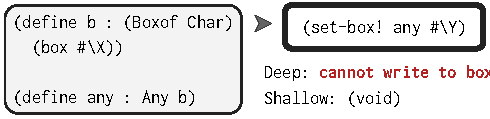
\includegraphics[trim=2.4000000000000004 2.4000000000000004 2.4000000000000004 2.4000000000000004]{pict_2.pdf}}}\end{FigureInside}\end{Centerfigure}

\Centertext{\Legend{\FigureTarget{\label{t:x28counter_x28x22figurex22_x22figx3aevaluationx3aanyx2dwrapx22x29x29}\textbf{Figure}~\textbf{14}: }{t:x28counter_x28x22figurex22_x22figx3aevaluationx3aanyx2dwrapx22x29x29}\textrm{Deep Racket enforces the top type (\Scribtexttt{Any}) with a contract that rejects all inputs}}}\end{Figure}

\Ssubsubsection{No Missing Wrappers}{No Missing Wrappers}\label{t:x28part_x22secx3aevaluationx3aexprx3awrapx22x29}

Mutable values that can appear in deep code need tailored
wrappers to monitor their interactions with non{-}deep clients.
These wrappers are difficult to implement because they often require support from the
run{-}time system\relax{~\citep{stff-oopsla-2012}}.
Unsurprisingly, some infrequently{-}used types in Deep Racket
lack wrappers (12 in total).

By contrast, a shallow language avoids the question of how
to implement wrappers.
Shallow types need only first{-}order checks, which require far
less engineering.

\Ssubsubsection{Uniform Behavior}{Uniform Behavior}\label{t:x28part_x22secx3aevaluationx3aexprx3auniformx22x29}

Although the purpose of deep wrappers is to reject type{-}incorrect
operations without otherwise changing behaviors,
certain wrappers in Deep Racket do cause subtle changes.
The most problematic ones are the wrappers for polymorphic types.
Deep Racket enforces types such as \Scribtexttt{(All (A) ({-}{\Stttextmore} A A))} with
a function contract that seals inputs and unseals outputs\relax{~\citep{gmfk-dls-2007}}.
The seals change the outcome of basic operations.

Shallow Racket avoids all such changes in behavior,
 including the well{-}known object identity issues\relax{~\citep{stff-oopsla-2012,kt-icfp-2015,vksb-dls-2014,vm-ecoop-2013}},
 because the transient semantics does not use wrappers.

\Ssubsection{Performance by Deep and Shallow}{Performance by Deep and Shallow}\label{t:x28part_x22secx3aevaluationx3aperformancex22x29}

The three{-}way mix of deep and shallow types improves performance
across the board.
On the GTP benchmark suite v6.0\relax{~\citep{gtp-bench6}},
toggling between deep and shallow avoids
pathological cases.
Mixing deep and shallow modules can further improve performance,
up to 2x faster than deep or shallow alone (relative to untyped code).

All data in this section was collected on a single{-}user Linux box
with 4 physical i7{-}4790 3.60GHz cores and 16GB RAM.
The machine ran Racket v7.8.0.5+\relax{~\citep{rkts}}
and a pre{-}release of Typed Racket\relax{~\citep{trs}}
that extends Typed Racket v1.12.
Each data point is the result of running one program configuration nine times in a row
 and averaging the speed of the final eight runs.
Our Racket\relax{~\citep{rkts}} does not optimize transient checks to the same extent as
a tracing JIT compiler (\ChapRef{\SectionNumberLink{t:x28part_x22secx3arelatedx22x29}{6}}{Related Work}), so there is potential room for
improvement.

\Ssubsubsection{Deep and Shallow Combined}{Deep and Shallow Combined}\label{t:x28part_x22secx3aevaluationx3aperfx3atogetherx22x29}

Mixing deep and shallow types within one program configuration can improve its
performance.
Such configurations are quite common in the GTP benchmarks.
Out of the \relax{$2^N$} configurations in sixteen of the smaller
benchmarks, a median of \relax{$37.5\%$} run fastest
with a mix of deep and shallow types (table~\hyperref[t:x28counter_x28x22figurex22_x22figx3abothx3a3wayx22x29x29]{\FigureRef{1}{t:x28counter_x28x22figurex22_x22figx3abothx3a3wayx22x29x29}}).
These mixtures also increase the number of \emph{\relax{$D$}{-}deliverable migration
paths} (defined in \SecRef{\SectionNumberLink{t:x28part_x22secx3aevaluationx3aperfx3apathx22x29}{5.3.4}}{Migration Paths}).
All paths in \relax{\textsf{fsm}}, \relax{\textsf{morsecode}}, \relax{\textsf{lnm}}, and \relax{\textsf{kcfa}} become \relax{$1.2$}{-}deliverable
when configurations can mix deep and shallow types.

These encouraging numbers are the result, however, of a search through
\relax{$3^N$} configurations.
The following three subsections therefore investigate Deep and Shallow
mixtures without relying on an exhaustive search.

\begin{table}\begin{Centerfigure}\begin{FigureInside}
  \Centertext{\Legend{\FigureTarget{\label{t:x28counter_x28x22figurex22_x22figx3abothx3a3wayx22x29x29}\textbf{Table}~\textbf{1}: }{t:x28counter_x28x22figurex22_x22figx3abothx3a3wayx22x29x29}\textrm{Percent of configurations that run fastest with a mix of Deep and Shallow modules.}}}
  \begin{SCentered}\begin{tabular}[t]{@{}l@{}l@{}l@{}}

\begin{tabular}[c]{@{}l@{}l@{}r@{}}
\hbox{Benchmark} &
\hbox{\mbox{\hphantom{\Scribtexttt{xx}}}} &
\hbox{Best w/ D+S} \\
\hline \hbox{\relax{\textsf{forth}}} &
\hbox{\mbox{\hphantom{\Scribtexttt{xx}}}} &
\hbox{12\%} \\
\hbox{\relax{\textsf{fsm}}} &
\hbox{\mbox{\hphantom{\Scribtexttt{xx}}}} &
\hbox{38\%} \\
\hbox{\relax{\textsf{fsmoo}}} &
\hbox{\mbox{\hphantom{\Scribtexttt{xx}}}} &
\hbox{31\%} \\
\hbox{\relax{\textsf{mbta}}} &
\hbox{\mbox{\hphantom{\Scribtexttt{xx}}}} &
\hbox{19\%} \\
\hbox{\relax{\textsf{morsecode}}} &
\hbox{\mbox{\hphantom{\Scribtexttt{xx}}}} &
\hbox{25\%} \\
\hbox{\relax{\textsf{zombie}}} &
\hbox{\mbox{\hphantom{\Scribtexttt{xx}}}} &
\hbox{6\%} \\
\hbox{\relax{\textsf{dungeon}}} &
\hbox{\mbox{\hphantom{\Scribtexttt{xx}}}} &
\hbox{31\%} \\
\hbox{\relax{\textsf{jpeg}}} &
\hbox{\mbox{\hphantom{\Scribtexttt{xx}}}} &
\hbox{38\%}\end{tabular} &
\hbox{\mbox{\hphantom{\Scribtexttt{xx}}}} &
\begin{tabular}[c]{@{}l@{}l@{}r@{}}
\hbox{Benchmark} &
\hbox{\mbox{\hphantom{\Scribtexttt{xx}}}} &
\hbox{Best w/ D+S} \\
\hline \hbox{\relax{\textsf{zordoz}}} &
\hbox{\mbox{\hphantom{\Scribtexttt{xx}}}} &
\hbox{47\%} \\
\hbox{\relax{\textsf{lnm}}} &
\hbox{\mbox{\hphantom{\Scribtexttt{xx}}}} &
\hbox{66\%} \\
\hbox{\relax{\textsf{suffixtree}}} &
\hbox{\mbox{\hphantom{\Scribtexttt{xx}}}} &
\hbox{48\%} \\
\hbox{\relax{\textsf{kcfa}}} &
\hbox{\mbox{\hphantom{\Scribtexttt{xx}}}} &
\hbox{55\%} \\
\hbox{\relax{\textsf{snake}}} &
\hbox{\mbox{\hphantom{\Scribtexttt{xx}}}} &
\hbox{46\%} \\
\hbox{\relax{\textsf{take5}}} &
\hbox{\mbox{\hphantom{\Scribtexttt{xx}}}} &
\hbox{36\%} \\
\hbox{\relax{\textsf{acquire}}} &
\hbox{\mbox{\hphantom{\Scribtexttt{xx}}}} &
\hbox{64\%} \\
\hbox{\relax{\textsf{tetris}}} &
\hbox{\mbox{\hphantom{\Scribtexttt{xx}}}} &
\hbox{62\%}\end{tabular}\end{tabular}\end{SCentered}\end{FigureInside}\end{Centerfigure}

\end{table}

\Ssubsubsection{Case Studies}{Case Studies}\label{t:x28part_x22secx3aevaluationx3aperfx3acasex22x29}

To test whether fast{-}running configurations can be found without a search,
we manually explored deep and shallow combinations in the following
programs:

\paragraph{MsgPack}
\href{https://gitlab.com/HiPhish/MsgPack.rkt}{MsgPack} is a Typed Racket
 library that converts Racket values into serialized
 \href{http://msgpack.org/}{MessagePack} data.\NoteBox{\NoteContent{\href{https://gitlab.com/HiPhish/MsgPack.rkt}{\Scribtexttt{gitlab{\hbox{\texttt{.}}}com/HiPhish/MsgPack{\hbox{\texttt{.}}}rkt}}}}
The author of this library
 \href{https://groups.google.com/g/racket-users/c/6KQxpfMLTn0/m/lil_6qSMDAAJ}{reported poor performance}
 due to deep type boundaries.
Changing a bridge module from deep to shallow types
(a one{-}line change),
reduces the time needed to run all tests from \relax{$320$} seconds to \relax{$204$} seconds
(\relax{$40\%$} speedup).

\paragraph{Synth}
The \relax{\textsf{synth}} benchmark is based on an untyped program
that interacts with a deep{-}typed math library to synthesize music.\NoteBox{\NoteContent{\href{https://github.com/stamourv/synth}{\Scribtexttt{github{\hbox{\texttt{.}}}com/stamourv/synth}}}}
This untyped program runs 14x slower than a deep{-}typed
version because of the library boundary.
When the library uses shallow types instead, the gap between an
untyped and deep{-}typed client improves to 5x.

\Ssubsubsection{Deep or Shallow, Worst{-}Case}{Deep or Shallow, Worst{-}Case}\label{t:x28part_x22secx3aevaluationx3aperfx3aeitherx2dorx22x29}

\begin{table}
\Centertext{\Legend{\FigureTarget{\label{t:x28counter_x28x22figurex22_x22figx3aevaluationx3amixedx2dworstx2dtablex22x29x29}\textbf{Table}~\textbf{2}: }{t:x28counter_x28x22figurex22_x22figx3aevaluationx3amixedx2dworstx2dtablex22x29x29}\textrm{Worst{-}case overheads vs. the untyped configuration for Deep alone, Shallow alone, and an either{-}or mix.}}}
  \begin{Centerfigure}\begin{FigureInside}
  \begin{SCentered}\begin{tabular}[t]{@{}l@{}l@{}r@{}r@{}r@{}r@{}r@{}}
\hbox{Benchmark} &
\hbox{\mbox{\hphantom{\Scribtexttt{xx}}}} &
\hbox{Worst Deep} &
\hbox{\mbox{\hphantom{\Scribtexttt{xx}}}} &
\hbox{Worst Shallow} &
\hbox{\mbox{\hphantom{\Scribtexttt{xx}}}} &
\hbox{Worst D$\parallel$S} \\
\hline \hbox{\relax{\textsf{sieve}}} &
\hbox{\mbox{\hphantom{\Scribtexttt{xx}}}} &
\hbox{16x} &
\hbox{\mbox{\hphantom{\Scribtexttt{xx}}}} &
\hbox{4.36x} &
\hbox{\mbox{\hphantom{\Scribtexttt{xx}}}} &
\hbox{\textbf{2.97x}} \\
\hbox{\relax{\textsf{forth}}} &
\hbox{\mbox{\hphantom{\Scribtexttt{xx}}}} &
\hbox{5800x} &
\hbox{\mbox{\hphantom{\Scribtexttt{xx}}}} &
\hbox{5.51x} &
\hbox{\mbox{\hphantom{\Scribtexttt{xx}}}} &
\hbox{\textbf{5.43x}} \\
\hbox{\relax{\textsf{fsm}}} &
\hbox{\mbox{\hphantom{\Scribtexttt{xx}}}} &
\hbox{2.24x} &
\hbox{\mbox{\hphantom{\Scribtexttt{xx}}}} &
\hbox{2.38x} &
\hbox{\mbox{\hphantom{\Scribtexttt{xx}}}} &
\hbox{\textbf{1.91x}} \\
\hbox{\relax{\textsf{fsmoo}}} &
\hbox{\mbox{\hphantom{\Scribtexttt{xx}}}} &
\hbox{420x} &
\hbox{\mbox{\hphantom{\Scribtexttt{xx}}}} &
\hbox{4.28x} &
\hbox{\mbox{\hphantom{\Scribtexttt{xx}}}} &
\hbox{\textbf{4.25x}} \\
\hbox{\relax{\textsf{mbta}}} &
\hbox{\mbox{\hphantom{\Scribtexttt{xx}}}} &
\hbox{1.91x} &
\hbox{\mbox{\hphantom{\Scribtexttt{xx}}}} &
\hbox{1.74x} &
\hbox{\mbox{\hphantom{\Scribtexttt{xx}}}} &
\hbox{\textbf{1.71x}} \\
\hbox{\relax{\textsf{morsecode}}} &
\hbox{\mbox{\hphantom{\Scribtexttt{xx}}}} &
\hbox{1.57x} &
\hbox{\mbox{\hphantom{\Scribtexttt{xx}}}} &
\hbox{2.77x} &
\hbox{\mbox{\hphantom{\Scribtexttt{xx}}}} &
\hbox{\textbf{1.3x}} \\
\hbox{\relax{\textsf{zombie}}} &
\hbox{\mbox{\hphantom{\Scribtexttt{xx}}}} &
\hbox{46x} &
\hbox{\mbox{\hphantom{\Scribtexttt{xx}}}} &
\hbox{31x} &
\hbox{\mbox{\hphantom{\Scribtexttt{xx}}}} &
\hbox{31x} \\
\hbox{\relax{\textsf{dungeon}}} &
\hbox{\mbox{\hphantom{\Scribtexttt{xx}}}} &
\hbox{15000x} &
\hbox{\mbox{\hphantom{\Scribtexttt{xx}}}} &
\hbox{4.97x} &
\hbox{\mbox{\hphantom{\Scribtexttt{xx}}}} &
\hbox{\textbf{3.16x}} \\
\hbox{\relax{\textsf{jpeg}}} &
\hbox{\mbox{\hphantom{\Scribtexttt{xx}}}} &
\hbox{23x} &
\hbox{\mbox{\hphantom{\Scribtexttt{xx}}}} &
\hbox{1.66x} &
\hbox{\mbox{\hphantom{\Scribtexttt{xx}}}} &
\hbox{\textbf{1.56x}} \\
\hbox{\relax{\textsf{zordoz}}} &
\hbox{\mbox{\hphantom{\Scribtexttt{xx}}}} &
\hbox{2.63x} &
\hbox{\mbox{\hphantom{\Scribtexttt{xx}}}} &
\hbox{2.75x} &
\hbox{\mbox{\hphantom{\Scribtexttt{xx}}}} &
\hbox{\textbf{2.58x}} \\
\hbox{\relax{\textsf{lnm}}} &
\hbox{\mbox{\hphantom{\Scribtexttt{xx}}}} &
\hbox{1.23x} &
\hbox{\mbox{\hphantom{\Scribtexttt{xx}}}} &
\hbox{1.21x} &
\hbox{\mbox{\hphantom{\Scribtexttt{xx}}}} &
\hbox{\textbf{1.17x}} \\
\hbox{\relax{\textsf{suffixtree}}} &
\hbox{\mbox{\hphantom{\Scribtexttt{xx}}}} &
\hbox{31x} &
\hbox{\mbox{\hphantom{\Scribtexttt{xx}}}} &
\hbox{5.8x} &
\hbox{\mbox{\hphantom{\Scribtexttt{xx}}}} &
\hbox{5.8x} \\
\hbox{\relax{\textsf{kcfa}}} &
\hbox{\mbox{\hphantom{\Scribtexttt{xx}}}} &
\hbox{4.33x} &
\hbox{\mbox{\hphantom{\Scribtexttt{xx}}}} &
\hbox{1.24x} &
\hbox{\mbox{\hphantom{\Scribtexttt{xx}}}} &
\hbox{1.24x} \\
\hbox{\relax{\textsf{snake}}} &
\hbox{\mbox{\hphantom{\Scribtexttt{xx}}}} &
\hbox{12x} &
\hbox{\mbox{\hphantom{\Scribtexttt{xx}}}} &
\hbox{7.67x} &
\hbox{\mbox{\hphantom{\Scribtexttt{xx}}}} &
\hbox{\textbf{7.61x}} \\
\hbox{\relax{\textsf{take5}}} &
\hbox{\mbox{\hphantom{\Scribtexttt{xx}}}} &
\hbox{44x} &
\hbox{\mbox{\hphantom{\Scribtexttt{xx}}}} &
\hbox{2.99x} &
\hbox{\mbox{\hphantom{\Scribtexttt{xx}}}} &
\hbox{\textbf{2.97x}} \\
\hbox{\relax{\textsf{acquire}}} &
\hbox{\mbox{\hphantom{\Scribtexttt{xx}}}} &
\hbox{4.22x} &
\hbox{\mbox{\hphantom{\Scribtexttt{xx}}}} &
\hbox{1.42x} &
\hbox{\mbox{\hphantom{\Scribtexttt{xx}}}} &
\hbox{1.42x} \\
\hbox{\relax{\textsf{tetris}}} &
\hbox{\mbox{\hphantom{\Scribtexttt{xx}}}} &
\hbox{13x} &
\hbox{\mbox{\hphantom{\Scribtexttt{xx}}}} &
\hbox{9.93x} &
\hbox{\mbox{\hphantom{\Scribtexttt{xx}}}} &
\hbox{\textbf{5.44x}} \\
\hbox{\relax{\textsf{synth}}} &
\hbox{\mbox{\hphantom{\Scribtexttt{xx}}}} &
\hbox{47x} &
\hbox{\mbox{\hphantom{\Scribtexttt{xx}}}} &
\hbox{4.2x} &
\hbox{\mbox{\hphantom{\Scribtexttt{xx}}}} &
\hbox{4.2x} \\
\hbox{\relax{\textsf{gregor}}} &
\hbox{\mbox{\hphantom{\Scribtexttt{xx}}}} &
\hbox{1.72x} &
\hbox{\mbox{\hphantom{\Scribtexttt{xx}}}} &
\hbox{1.59x} &
\hbox{\mbox{\hphantom{\Scribtexttt{xx}}}} &
\hbox{\textbf{1.51x}} \\
\hbox{\relax{\textsf{quadT}}} &
\hbox{\mbox{\hphantom{\Scribtexttt{xx}}}} &
\hbox{26x} &
\hbox{\mbox{\hphantom{\Scribtexttt{xx}}}} &
\hbox{7.39x} &
\hbox{\mbox{\hphantom{\Scribtexttt{xx}}}} &
\hbox{\textbf{7.23x}} \\
\hbox{\relax{\textsf{quadU}}} &
\hbox{\mbox{\hphantom{\Scribtexttt{xx}}}} &
\hbox{55x} &
\hbox{\mbox{\hphantom{\Scribtexttt{xx}}}} &
\hbox{7.57x} &
\hbox{\mbox{\hphantom{\Scribtexttt{xx}}}} &
\hbox{\textbf{7.45x}}\end{tabular}\end{SCentered}\end{FigureInside}\end{Centerfigure}

\end{table}

\noindent Both deep and shallow implementations have known bottlenecks.
With deep types, high{-}traffic boundaries can lead to huge
costs\relax{~\citep{htf-hosc-2010,tfgnvf-popl-2016,gtnffvf-jfp-2019}}.
With shallow types, every line of typed code contributes a small
cost\relax{~\citep{vss-popl-2017,gm-pepm-2018}}.

By switching between Deep and Shallow a programmer can often, however,
avoid the worst{-}cases of each.
Table~\hyperref[t:x28counter_x28x22figurex22_x22figx3aevaluationx3amixedx2dworstx2dtablex22x29x29]{\FigureRef{2}{t:x28counter_x28x22figurex22_x22figx3aevaluationx3amixedx2dworstx2dtablex22x29x29}} quantifies the benefits of
this either{-}or strategy on the GTP benchmarks.
The first column shows that, as expected, deep types may have
enormous costs.
The second column shows that the worst configurations for Shallow Racket are
far less severe.
The third column shows, however, that toggling between Deep and Shallow
often avoids the pathologies of each style.
Numbers in this third column are typeset in \textbf{bold} if they
are the best (lowest) in their row.

\emph{Remark:} the either{-}or {``}toggling{''} strategy is possible only
because Deep and Shallow can interoperate.
Most of the benchmarks rely on deep{-}typed
code that lives outside their \relax{$N$} core migratable modules (16 out of 21 benchmarks).
Without interoperability, the outside code would require changes that are
unrealistic to make in practice.

In table~\hyperref[t:x28counter_x28x22figurex22_x22figx3aevaluationx3amixedx2dworstx2dtablex22x29x29]{\FigureRef{2}{t:x28counter_x28x22figurex22_x22figx3aevaluationx3amixedx2dworstx2dtablex22x29x29}}, the \Scribtexttt{sieve} and
\Scribtexttt{tetris} benchmarks are notable successes.
The \Scribtexttt{zombie} benchmark is the worst.
Deep Racket pays a huge cost in \Scribtexttt{zombie} because functions
repeatedly cross its module boundaries.
Shallow Racket pays a high cost as well because \Scribtexttt{zombie}
uses functions to simulate message{-}passing objects, and therefore contains
many elimination forms that incur shape checks.


\Ssubsubsection{Migration Paths}{Migration Paths}\label{t:x28part_x22secx3aevaluationx3aperfx3apathx22x29}

\begin{table}
  \begin{Centerfigure}\begin{FigureInside}
\Centertext{\Legend{\FigureTarget{\label{t:x28counter_x28x22figurex22_x22figx3abothx3amixedx2dpathx22x29x29}\textbf{Table}~\textbf{3}: }{t:x28counter_x28x22figurex22_x22figx3abothx3amixedx2dpathx22x29x29}\textrm{Percent of \relax{$3$}{-}deliverable migration paths for Deep alone, Shallow alone, and an either{-}or mix.}}}

    \begin{SCentered}\begin{tabular}[t]{@{}l@{}l@{}r@{}r@{}r@{}r@{}r@{}}
\hbox{Benchmark} &
\hbox{\mbox{\hphantom{\Scribtexttt{xx}}}} &
\hbox{Deep paths} &
\hbox{\mbox{\hphantom{\Scribtexttt{xx}}}} &
\hbox{Shallow paths} &
\hbox{\mbox{\hphantom{\Scribtexttt{xx}}}} &
\hbox{D$\parallel$S paths} \\
\hline \hbox{\relax{\textsf{sieve}}} &
\hbox{\mbox{\hphantom{\Scribtexttt{xx}}}} &
\hbox{0\%} &
\hbox{\mbox{\hphantom{\Scribtexttt{xx}}}} &
\hbox{0\%} &
\hbox{\mbox{\hphantom{\Scribtexttt{xx}}}} &
\hbox{\textbf{100\%}} \\
\hbox{\relax{\textsf{forth}}} &
\hbox{\mbox{\hphantom{\Scribtexttt{xx}}}} &
\hbox{0\%} &
\hbox{\mbox{\hphantom{\Scribtexttt{xx}}}} &
\hbox{0\%} &
\hbox{\mbox{\hphantom{\Scribtexttt{xx}}}} &
\hbox{\textbf{50\%}} \\
\hbox{\relax{\textsf{fsm}}} &
\hbox{\mbox{\hphantom{\Scribtexttt{xx}}}} &
\hbox{100\%} &
\hbox{\mbox{\hphantom{\Scribtexttt{xx}}}} &
\hbox{100\%} &
\hbox{\mbox{\hphantom{\Scribtexttt{xx}}}} &
\hbox{100\%} \\
\hbox{\relax{\textsf{fsmoo}}} &
\hbox{\mbox{\hphantom{\Scribtexttt{xx}}}} &
\hbox{0\%} &
\hbox{\mbox{\hphantom{\Scribtexttt{xx}}}} &
\hbox{0\%} &
\hbox{\mbox{\hphantom{\Scribtexttt{xx}}}} &
\hbox{\textbf{50\%}} \\
\hbox{\relax{\textsf{mbta}}} &
\hbox{\mbox{\hphantom{\Scribtexttt{xx}}}} &
\hbox{100\%} &
\hbox{\mbox{\hphantom{\Scribtexttt{xx}}}} &
\hbox{100\%} &
\hbox{\mbox{\hphantom{\Scribtexttt{xx}}}} &
\hbox{100\%} \\
\hbox{\relax{\textsf{morsecode}}} &
\hbox{\mbox{\hphantom{\Scribtexttt{xx}}}} &
\hbox{100\%} &
\hbox{\mbox{\hphantom{\Scribtexttt{xx}}}} &
\hbox{100\%} &
\hbox{\mbox{\hphantom{\Scribtexttt{xx}}}} &
\hbox{100\%} \\
\hbox{\relax{\textsf{zombie}}} &
\hbox{\mbox{\hphantom{\Scribtexttt{xx}}}} &
\hbox{0\%} &
\hbox{\mbox{\hphantom{\Scribtexttt{xx}}}} &
\hbox{0\%} &
\hbox{\mbox{\hphantom{\Scribtexttt{xx}}}} &
\hbox{\textbf{50\%}} \\
\hbox{\relax{\textsf{dungeon}}} &
\hbox{\mbox{\hphantom{\Scribtexttt{xx}}}} &
\hbox{0\%} &
\hbox{\mbox{\hphantom{\Scribtexttt{xx}}}} &
\hbox{0\%} &
\hbox{\mbox{\hphantom{\Scribtexttt{xx}}}} &
\hbox{\textbf{67\%}} \\
\hbox{\relax{\textsf{jpeg}}} &
\hbox{\mbox{\hphantom{\Scribtexttt{xx}}}} &
\hbox{0\%} &
\hbox{\mbox{\hphantom{\Scribtexttt{xx}}}} &
\hbox{100\%} &
\hbox{\mbox{\hphantom{\Scribtexttt{xx}}}} &
\hbox{100\%} \\
\hbox{\relax{\textsf{zordoz}}} &
\hbox{\mbox{\hphantom{\Scribtexttt{xx}}}} &
\hbox{100\%} &
\hbox{\mbox{\hphantom{\Scribtexttt{xx}}}} &
\hbox{100\%} &
\hbox{\mbox{\hphantom{\Scribtexttt{xx}}}} &
\hbox{100\%} \\
\hbox{\relax{\textsf{lnm}}} &
\hbox{\mbox{\hphantom{\Scribtexttt{xx}}}} &
\hbox{100\%} &
\hbox{\mbox{\hphantom{\Scribtexttt{xx}}}} &
\hbox{100\%} &
\hbox{\mbox{\hphantom{\Scribtexttt{xx}}}} &
\hbox{100\%} \\
\hbox{\relax{\textsf{suffixtree}}} &
\hbox{\mbox{\hphantom{\Scribtexttt{xx}}}} &
\hbox{0\%} &
\hbox{\mbox{\hphantom{\Scribtexttt{xx}}}} &
\hbox{0\%} &
\hbox{\mbox{\hphantom{\Scribtexttt{xx}}}} &
\hbox{\textbf{12\%}} \\
\hbox{\relax{\textsf{kcfa}}} &
\hbox{\mbox{\hphantom{\Scribtexttt{xx}}}} &
\hbox{33\%} &
\hbox{\mbox{\hphantom{\Scribtexttt{xx}}}} &
\hbox{100\%} &
\hbox{\mbox{\hphantom{\Scribtexttt{xx}}}} &
\hbox{100\%} \\
\hbox{\relax{\textsf{snake}}} &
\hbox{\mbox{\hphantom{\Scribtexttt{xx}}}} &
\hbox{0\%} &
\hbox{\mbox{\hphantom{\Scribtexttt{xx}}}} &
\hbox{0\%} &
\hbox{\mbox{\hphantom{\Scribtexttt{xx}}}} &
\hbox{0\%} \\
\hbox{\relax{\textsf{take5}}} &
\hbox{\mbox{\hphantom{\Scribtexttt{xx}}}} &
\hbox{0\%} &
\hbox{\mbox{\hphantom{\Scribtexttt{xx}}}} &
\hbox{100\%} &
\hbox{\mbox{\hphantom{\Scribtexttt{xx}}}} &
\hbox{100\%}\end{tabular}\end{SCentered}\end{FigureInside}\end{Centerfigure}

\end{table}

\noindent The complementary strengths of Deep and Shallow Racket can help
programmers avoid bottlenecks as they migrate an untyped codebase to a
typed configuration.
Consider the set of all migration paths, each of which begins at the
untyped configuration and adds types to one module at a time until
reaching the fully{-}typed configuration.
A path is \relax{$D$}{-}deliverable if all of its configurations
run at most \relax{$D$} times slower than the untyped configuration.

Table~\hyperref[t:x28counter_x28x22figurex22_x22figx3abothx3amixedx2dpathx22x29x29]{\FigureRef{3}{t:x28counter_x28x22figurex22_x22figx3abothx3amixedx2dpathx22x29x29}} counts the proportion of \relax{$3$}{-}deliverable
paths out of all \relax{$N!$} migration paths in a subset of the GTP benchmarks.
Larger benchmarks are omitted.
The first column counts paths in Deep Racket,
the second column counts paths in Shallow Racket, and
the third column counts paths using Deep or Shallow at each point.
With Deep alone, all paths in nine
benchmarks reach a bottleneck that exceeds the 3x limit.
With Shallow alone, all paths in seven benchmarks
 exceed the limit as well{---}often near the end of the migration path.
With the either{-}or mix, only one benchmark (\relax{\textsf{snake}})
 has zero \relax{$3$}{-}deliverable paths.

\sectionNewpage

\Ssection{Related Work}{Related Work}\label{t:x28part_x22secx3arelatedx22x29}

Two gradual languages, Thorn\relax{~\citep{wzlov-popl-2010}} and
StrongScript\relax{~\citep{rzv-ecoop-2015}}, support a combination of sound
\emph{concrete} types and erased \emph{like} types.
Thorn is a scalable scripting language that compiles to the JVM\relax{~\citep{bfnorsvw-oopsla-2009}}.
StrongScript extends TypeScript\relax{~\citep{bat-ecoop-2014}} with concrete types.
Pyret explores a type{-}based combination, with deep checks for types that
describe fixed{-}size data and shallow checks for other types.\NoteBox{\NoteContent{Personal
communication.  \href{https://www.pyret.orgpyret.org}{\Scribtexttt{pyret{\hbox{\texttt{.}}}org}}}}
For example, pair types get a deep check and list types get a shallow
check.
Static Python combines shallow and concrete checks\relax{~\citep{lgmvpk-draft-2022}}.
Shallow checks are the default, and programmers can opt{-}in to concrete
data structures.
Outside the realm of gradual typing, option contracts allow client code to trust
(and skip checking) specific contracts from server code\relax{~\citep{dff-oopsla-2013}}.

The model in \ChapRef{\SectionNumberLink{t:x28part_x22secx3amodelx22x29}{3}}{Model and Metatheory} builds on the semantic framework
of \relax{\citet{gf-icfp-2018}}, which is in turn inspired by
\relax{\citet{mf-toplas-2009}}.
Unlike those frameworks, the present model uses a surface{-}to{-}evaluation compiler
similar to how \relax{\citet{clzv-ecoop-2018}} compile several gradual languages to
the \relax{\kafka} core language.
The compiler in \ChapRef{\SectionNumberLink{t:x28part_x22secx3amodelx22x29}{3}}{Model and Metatheory} is inspired by the coercion calculus\relax{~\citep{h-scp-1994}};
in particular, its \emph{completion} pass that makes run{-}time type checks explicit.

There is a great deal of related work that addresses the performance of
deep or shallow types via implementation techniques\relax{~\citep{fgsfs-oopsla-2018}},
static analysis\relax{~\citep{ngtv-popl-2018,ngtv-pldi-2019,vsc-dls-2019,mntv-popl-2021}},
compilation techniques\relax{~\citep{bbst-oopsla-2017,rat-oopsla-2017,rmhn-ecoop-2019}},
and clean{-}slate language designs\relax{~\citep{mt-oopsla-2017,kas-pldi-2019,mt-oopsla-2021}}.
These improvements are orthogonal to a combined language; they should
apply to a three{-}way language as well as any normal gradual language.
As a case in point, our three{-}way Typed Racket
benefits from collapsible contracts\relax{~\citep{fgsfs-oopsla-2018}}.

\sectionNewpage

\Ssection{Future Work}{Future Work}\label{t:x28part_x22secx3afuturex22x29}

One drawback apparent in the model is that deep and shallow cannot
trust one another.
Deep code always wraps inputs from shallow code because they may have
originated in untyped code.
\relax{\citet{g-thesis-2020}} sketches two ideas for removing checks from
deep{--}shallow boundaries.
One requires an escape analysis.
The other asks for a shallow semantics that creates wrappers
(such as in \relax{~\citep{cl-icfp-2017}})
instead of the transient semantics.
A third idea is to adapt confined gradual typing\relax{~\citep{afgt-oopsla-2014}}.
If the type system can prove that confined values originate in typed code and
never escape to untyped, then deep and shallow can freely share these
values.

A second future direction is to identify best practices for coding in
a three{-}way language.
Anecdotal experience suggests the following strategy:


\noindent \begin{enumerate}\atItemizeStart

\item Start by adding deep types because their strong guarantees may help
identify logical errors.

\item If performance becomes an issue, switch to shallow.

\item Once all critical boundaries are typed, use deep to maximize
the effect of type{-}driven optimizations.\end{enumerate}

\noindent \noindent{}Adapting the notion of a \emph{rational
programmer}\relax{~\citep{lgfd-icfp-2021}} may provide a way to systematically test the
usefulness of this migration plan.
Meanwhile, there may be additional ways to leverage the spectrum of type
enforcement.

\sectionNewpage

\Ssection{Conclusion}{Conclusion}\label{t:x28part_x22secx3aconclusionx22x29}

This is the first implementation of a sound gradual type system where
programmers can explicitly choose to trade performance for guarantees
as they add types.
If a new set of type annotations brings unacceptable overhead,
switching the types{'} semantics from deep to shallow
can avoid the bottleneck and may even be good enough to deploy.
The guarantees from deep types can always be used for debugging
the inevitable failure, and can be applied sparingly to defend
a critical module.
In the future, implementors may wish to explore other ways to trade
performance for guarantees, making the trade{-}off even more programmable.

\section*{Data Availability Statement}

The datasets and software that support
section~\ref{t:x28part_x22secx3aevaluationx22x29} of this paper
are available via Software Heritage~\cite{gpldi2022sh}
and Zenodo~\cite{gpldi2022z}.


\begin{acks}

This work is supported by
\href{https://www.nsf.gov/awardsearch/showAward?AWD_ID=1518844}{NSF grant 1518844}
and
\href{https://www.nsf.gov/awardsearch/showAward?AWD_ID=2030859}{NSF grant 2030859}
to the CRA for the \href{https://cifellows2020.org}{CIFellows} project.
Thanks to Matthias Felleisen for improving drafts of this paper and to
the rest of my thesis committee for supervising parts of this work:
Amal Ahmed,
Fritz Henglein,
Shriram Krishnamurthi,
Sam Tobin{-}Hochstadt,
and
Jan Vitek.

\end{acks}

\relax{\begingroup
\setlength{\emergencystretch}{8em}
\balance
\printbibliography
\endgroup}

\postDoc
\end{document}
